\documentclass[dissertation,appendmultiple]{MSUstyle}
%
%  Created by Seth Humphries 
%  Update and maintained by Prof. Mark Owkes mark.owkes@montana.edu
% 
%%    Copyright (c) 2007-2012 Seth D. Humphries
%%    This work is licensed under the Creative Commons
%%    Attribution-Noncommercial-Share Alike 3.0 License. To view a copy
%%    of this license, visit http://creativecommons.org/licenses/by-nc-sa/3.0/;
%%    or, (b) send a letter to Creative Commons, 171 2nd Street, Suite
%%    300, San Francisco, California, 94105, USA. 
%
%  Version 2.0, check for periodic updates on the bitbucket repository
%
% DEFAULTS --------------------
% The default options are as follows:
%   \documentclass[12pt,letterpaper,oneside,openright,%
%       doublespaced,normalmargins,dissertation,final,numreset]{MSUstyle}
%
% default options do not need to be entered. Defaults will generate a document 
% that conforms to the MSU Electronic Thesis/Dissertation  (ETD) guidelines. 
%
% MASTERS THESIS ---------------
%  use \documentclass[thesis]{MSUstyle} to adjustment the front matter according to ETD style rules that
% are different for a thesis than for a dissertation.
%
% ADDITIONAL OPTIONS ----------
% 10pt, singlespaced, and draft allow you to require less number of pages for editing
% A draft version number can be set with, e.g., \draftver{1.0}
%
% numberedsections provides numbered chapter and section titles
%
% appendsingle/appendmultiple is required if you have one/multiple appendices, remove if you do not have an appendix
%
% nonumreset does not add chapter to labels of figures, tables, etc. (not recommended)
%
% PRINTING OPTIONS ------------
% oneside,openright (defaults) 1" margin on all sides of pages (use for electronic documents and submission to grad school)
% oneside,openright,bigmargin larger margin on left side of pages (optionally use for electronic documents and submission to grad school)
% twoside,openany  larger margins alternate left/right sides for binding (use for printing on minimal number of pages)
% twoside,openright larger margins alternate left/right sides for binding and ...
%                               blank pages added so chapter start on right page (use for nicest printed material)

% ========================= %
%  Packages                 %
%  (add as needed)          %
% ========================= %


%% FRAMINGS PACKAGES
%\usepackage{amsmath}
\usepackage{amsfonts}
\usepackage{amssymb}
\usepackage{amsthm}
\usepackage{comment}
\usepackage{epsfig}
\usepackage{psfrag}
\usepackage{mathrsfs}
\usepackage{amscd}
\usepackage[all]{xy}
\usepackage{rotating}
\usepackage{lscape}
\usepackage{amsbsy}
\usepackage{verbatim}
\usepackage{moreverb}
\usepackage{color} 


\usepackage{bbm}
\usepackage{eucal}
\usepackage{stackrel}
\usepackage{stmaryrd}

\usepackage{tikz-cd}
%\usetikzlibrary{patterns,shapes.geometric,arrows,decorations.markings}
%\usepackage{tikz-3dplot}

\usepackage{caption}
%\usepackage{subcaption}

%\colorlet{lightgray}{black!15}

%\tikzset{->-/.style={decoration={
  %markings,
  %mark=at position .5 with {\arrow{>}}},postaction={decorate}}}
%\tikzset{midarrow/.style={decoration={
   % markings,
   % mark=at position {#1} with {\arrow{>}}},postaction={decorate}} }





%%%%%


%\usepackage[final]{graphicx} %for the \includegraphics command and figures put [final] before ...
%%    {graphix} if you want figures to show up even while in draft mode
\usepackage{subcaption}    % to be able to have multiple plots in one figure
\usepackage{color} % for changing text color in chapters \textcolor{red}{red text read here}. 
\usepackage{varioref}  % for \vref{figure} which shows up like ``figure 4 on page 6'' 
\usepackage[final]{listings} % used for formatting code
\usepackage[pdftex,hidelinks]{hyperref}
\usepackage{cite} %compresses the citations so \cite{ref1,ref2,ref3,ref4} is printed as [1-4] instead of [1,2,3,4]
\usepackage[]{natbib} % for citations

\usepackage{tikz} % used for creating figures
\usetikzlibrary{calc}
\usetikzlibrary{patterns}
\usetikzlibrary{positioning}
\usetikzlibrary{decorations.markings}
\usetikzlibrary{decorations.pathmorphing}
\usetikzlibrary{arrows}
\usepackage{array}
\usepackage{amsmath}
\usepackage{lipsum} % Generates random text
%\usepackage{showframe} % View margins


 

\usepackage{mathtools}
% Style of code listings (Change as needed)
\lstset{%set Code listings styles
	language=Matlab, % program language for keywords and comments styles
	basicstyle=\small, %font size and style
	identifierstyle=\color{red}, %variable name style
	stringstyle=\ttfamily, %string style
	keywordstyle=\color{blue}\bfseries, %language keyword style
	commentstyle=\color{black}\itshape, %commentstyle
	breaklines=true,  % sets automatic line breaking
	breakatwhitespace=false,   %break line not just at whitespaces
}


% ======================= %
%  User defined commands  %
% ======================= %


\newtheorem{maintheorem}{Theorem}[section]
\renewcommand*{\themaintheorem}{\Alph{maintheorem}}

\newtheorem{theorem}{Theorem}[section]
\newtheorem{innercustomthm}{Theorem}
\newenvironment{mythm}[1]
  {\renewcommand\theinnercustomthm{#1}\innercustomthm}
  {\endinnercustomthm}


%\newtheorem{theorem}{Theorem}[section]
\newtheorem{prop}[theorem]{Proposition}
\newtheorem{lemma}[theorem]{Lemma}
\newtheorem{cor}[theorem]{Corollary}
\newtheorem{conj}{Conjecture}




\theoremstyle{definition}
\newtheorem{definition}[theorem]{Definition}
\newtheorem{summary}[theorem]{Summary}
\newtheorem{note}[theorem]{Note}
\newtheorem{ack}[theorem]{Acknowledgments}
\newtheorem{observation}[theorem]{Observation}
\newtheorem{construction}[theorem]{Construction}
\newtheorem{terminology}[theorem]{Terminology}
\newtheorem{remark}[theorem]{Remark}
\newtheorem{problem}[theorem]{Problem}
\newtheorem{example}[theorem]{Example}
\newtheorem{q}[theorem]{Question}
\newtheorem{notation}[theorem]{Notation}
\newtheorem{criterion}[theorem]{Criterion}
\newtheorem*{conventions*}{Conventions}
\newtheorem{convention}{Convention}
\newtheorem{claim}[theorem]{Claim}
\newtheorem{warning}[theorem]{Warning}



\theoremstyle{remark}


\definecolor{orange}{rgb}{.95,0.5,0}
\definecolor{light-gray}{gray}{0.75}
\definecolor{brown}{cmyk}{0, 0.8, 1, 0.6}
\definecolor{plum}{rgb}{.5,0,1}


\DeclareMathOperator{\Link}{\sf Link}
\DeclareMathOperator{\Fin}{\sf Fin}
\DeclareMathOperator{\vect}{\sf Vect}
\DeclareMathOperator{\Vect}{\cV{\sf ect}}
\DeclareMathOperator{\Sfr}{S-{\sf fr}}
\DeclareMathOperator{\nfr}{\mathit{n}-{\sf fr}}

\DeclareMathOperator{\pr}{\mathsf{pr}}
\DeclareMathOperator{\ev}{\mathsf{ev}}


\DeclareMathOperator{\bBar}{\sf Bar}
\DeclareMathOperator{\Alg}{\sf Alg}
\DeclareMathOperator{\man}{\sf Man}
\DeclareMathOperator{\Man}{\cM{\sf an}}
\DeclareMathOperator{\Mod}{\sf Mod}
\DeclareMathOperator{\unzip}{\sf Unzip}
\DeclareMathOperator{\Snglr}{\cS{\sf nglr}}
\DeclareMathOperator{\TwAr}{\sf TwAr}

\DeclareMathOperator{\cSpan}{\sf cSpan}
\DeclareMathOperator{\Kan}{\sf Kan}
\DeclareMathOperator{\Psh}{\sf PShv}
\DeclareMathOperator{\LFib}{\sf LFib}
\DeclareMathOperator{\CAlg}{\sf CAlg}


\DeclareMathOperator{\cpt}{\sf cpt}
\DeclareMathOperator{\Aut}{\sf Aut}
\DeclareMathOperator{\colim}{{\sf colim}}
\DeclareMathOperator{\relcolim}{{\sf rel.\!colim}}
\DeclareMathOperator{\limit}{{\sf lim}}
\DeclareMathOperator{\cone}{\sf cone}
\DeclareMathOperator{\Der}{\sf Der}
\DeclareMathOperator{\Ext}{\sf Ext}
\DeclareMathOperator{\hocolim}{\sf hocolim}
\DeclareMathOperator{\holim}{\sf holim}
\DeclareMathOperator{\Hom}{\sf Hom}
\DeclareMathOperator{\End}{\sf End}
\DeclareMathOperator{\ulhom}{\underline{\Hom}}
\DeclareMathOperator{\fun}{\sf Fun}
\DeclareMathOperator{\Fun}{{\sf Fun}}
\DeclareMathOperator{\Iso}{\sf Iso}
\DeclareMathOperator{\map}{\sf Map}
\DeclareMathOperator{\Map}{{\sf Map}}
\DeclareMathOperator{\Mapc}{{\sf Map}_{\sf c}}
\DeclareMathOperator{\Gammac}{{\Gamma}_{\!\sf c}}
\DeclareMathOperator{\Tot}{\sf Tot}
\DeclareMathOperator{\Spec}{\sf Spec}
\DeclareMathOperator{\Spf}{\sf Spf}
\DeclareMathOperator{\Def}{\sf Def}
\DeclareMathOperator{\stab}{\sf Stab}
\DeclareMathOperator{\costab}{\sf Costab}
\DeclareMathOperator{\ind}{\sf Ind}
\DeclareMathOperator{\coind}{\sf Coind}
\DeclareMathOperator{\res}{\sf Res}
\DeclareMathOperator{\Ker}{\sf Ker}
\DeclareMathOperator{\coker}{\sf Coker}
\DeclareMathOperator{\pt}{\sf pt}
\DeclareMathOperator{\Sym}{\sf Sym}

\DeclareMathOperator{\str}{\sf str}

\DeclareMathOperator{\exit}{\sf Exit}
\DeclareMathOperator{\Exit}{\bcE{\sf xit}}

\DeclareMathOperator{\cylr}{{\sf Cylr}}

\DeclareMathOperator{\shift}{\sf shift}

\newcommand{\bit}[1]{\textbf{\textit{#1}}}
\newcommand{\racts}{\curvearrowleft}
\newcommand{\lacts}{\curvearrowright}




\DeclareMathOperator{\Cat}{{\sf Cat}}
\DeclareMathOperator{\fCat}{{\sf fCat}}
\DeclareMathOperator{\cat}{\fC{\sf at}}
\DeclareMathOperator{\Gcat}{{\sf GCat}_{\oo}}
\DeclareMathOperator{\gcat}{{\sf GCat}}
\DeclareMathOperator{\Dcat}{{\sf GCat}}
\DeclareMathOperator{\dcat}{\fG\fC{\sf at}}
\DeclareMathOperator{\Mcat}{\cM{\sf Cat}}
\DeclareMathOperator{\mcat}{\fD{\sf Cat}}






\DeclareMathOperator{\Ar}{{\sf Ar}}
\DeclareMathOperator{\twar}{{\sf TwAr}}


\DeclareMathOperator{\diskcat}{\sf {\cD}isk_{\mathit n}^\tau-Cat_\infty}
\DeclareMathOperator{\mfdcat}{\sf {\cM}fd_{\mathit n}^\tau-Cat_\infty}
\DeclareMathOperator{\diskone}{\sf {\cD}isk_{1}^{\vfr}-Cat_\infty}

\DeclareMathOperator{\symcat}{\sf Sym-Cat_\infty}
\DeclareMathOperator{\encat}{\cE_{\mathit n}-\sf Cat}
\DeclareMathOperator{\moncat}{\sf Mon-Cat_\infty}

\DeclareMathOperator{\inrshv}{\sf inr-shv}
\DeclareMathOperator{\clsshv}{\sf cls-shv}



\DeclareMathOperator{\qc}{\sf QC}
\DeclareMathOperator{\m}{\sf Mod}
\DeclareMathOperator{\bi}{\sf Bimod}
\DeclareMathOperator{\perf}{\sf Perf}
\DeclareMathOperator{\shv}{\sf Shv}
\DeclareMathOperator{\Shv}{\sf Shv}



\DeclareMathOperator{\psh}{\sf PShv}
\DeclareMathOperator{\gshv}{\sf GShv}
\DeclareMathOperator{\csh}{\sf Coshv}
\DeclareMathOperator{\comod}{\sf Comod}
\DeclareMathOperator{\M}{\mathsf{-Mod}}
\DeclareMathOperator{\coalg}{\mathsf{-coalg}}
\DeclareMathOperator{\ring}{\mathsf{-rings}}
\DeclareMathOperator{\alg}{\mathsf{Alg}}
\DeclareMathOperator{\artin}{{\sf Artin}}%{\disk_{\mathit n}\alg^{\sf Art}_{\mathit k}}
\DeclareMathOperator{\art}{\mathsf{Art}}
\DeclareMathOperator{\triv}{\mathsf{Triv}}
\DeclareMathOperator{\cobar}{\mathsf{cBar}}
\DeclareMathOperator{\ba}{\mathsf{Bar}}

\DeclareMathOperator{\shvp}{\sf Shv_{\sf p}^{\sf cbl}}

\DeclareMathOperator{\lkan}{{\sf LKan}}
\DeclareMathOperator{\rkan}{{\sf RKan}}

\DeclareMathOperator{\Diff}{{\sf Diff}}
\DeclareMathOperator{\sh}{\sf shv}



\DeclareMathOperator{\calg}{\mathsf{CAlg}}
\DeclareMathOperator{\op}{\mathsf{op}}
\DeclareMathOperator{\relop}{\mathsf{rel.op}}
\DeclareMathOperator{\com}{\mathsf{Com}}
\DeclareMathOperator{\bu}{\cB\mathsf{un}}
\DeclareMathOperator{\bun}{\sf Bun}

\DeclareMathOperator{\pbun}{\sf PBun}




\DeclareMathOperator{\cMfld}{{\sf c}\cM\mathsf{fld}}
\DeclareMathOperator{\cBun}{{\sf c}\cB\mathsf{un}}
\DeclareMathOperator{\Bun}{\cB\mathsf{un}}

\DeclareMathOperator{\dbu}{\mathsf{DBun}}

\DeclareMathOperator{\dbun}{\mathsf{DBun}}

\DeclareMathOperator{\bsc}{\mathsf{Bsc}}
\DeclareMathOperator{\snglr}{\sf Snglr}

\DeclareMathOperator{\Bsc}{\cB\mathsf{sc}}


\DeclareMathOperator{\arbr}{\mathsf{Arbr}}
\DeclareMathOperator{\Arbr}{\cA\mathsf{rbr}}
\DeclareMathOperator{\Rf}{\cR\mathsf{ef}}
\DeclareMathOperator{\drf}{\mathsf{Ref}}


\DeclareMathOperator{\st}{\mathsf{st}}
\DeclareMathOperator{\sk}{\mathsf{sk}}
\DeclareMathOperator{\Ex}{\mathsf{Ex}}

\DeclareMathOperator{\sd}{\mathsf{sd}}

\DeclareMathOperator{\inr}{\mathsf{inr}}

\DeclareMathOperator{\cls}{\mathsf{cls}}
\DeclareMathOperator{\act}{\mathsf{act}}
\DeclareMathOperator{\rf}{\mathsf{ref}}
\DeclareMathOperator{\pcls}{\mathsf{pcls}}
\DeclareMathOperator{\opn}{\mathsf{open}}
\DeclareMathOperator{\emb}{\mathsf{emb}}
\DeclareMathOperator{\Cylo}{\mathsf{Cylo}}
\DeclareMathOperator{\Cylr}{\mathsf{Cylr}}


\DeclareMathOperator{\cbl}{\mathsf{cbl}}

\DeclareMathOperator{\pcbl}{\mathsf{p.cbl}}


\DeclareMathOperator{\gl}{\mathsf{GL}_1}

\DeclareMathOperator{\Top}{\mathsf{Top}}
\DeclareMathOperator{\Mfd}{{\cM}\mathsf{fd}}
\DeclareMathOperator{\cMfd}{{\sf c}{\cM}\mathsf{fd}}
\DeclareMathOperator{\Mfld}{{\sf Mfld}}
\DeclareMathOperator{\mfd}{\mathsf{Mfd}}
\DeclareMathOperator{\Emb}{\mathsf{Emb}}
\DeclareMathOperator{\enr}{\fE\mathsf{nr}}
\DeclareMathOperator{\LEnr}{\mathsf{LEnr}}
\DeclareMathOperator{\diff}{\mathsf{Diff}}
\DeclareMathOperator{\conf}{\mathsf{Conf}}

\DeclareMathOperator{\MC}{\mathsf{MC}}
\DeclareMathOperator{\strat}{\mathsf{Strat}}
\DeclareMathOperator{\Strat}{\cS\mathsf{trat}}
\DeclareMathOperator{\kan}{\mathsf{Kan}}

\DeclareMathOperator{\dd}{{\cD}\mathsf{isk}}

\DeclareMathOperator{\loc}{\mathsf{Loc}}



\DeclareMathOperator{\poset}{\mathsf{Poset}}



\DeclareMathOperator{\spaces}{\cS\mathsf{paces}}
\DeclareMathOperator{\Spaces}{\cS\mathsf{paces}}
\DeclareMathOperator{\Sets}{\cS\mathsf{ets}}

\DeclareMathOperator{\Space}{{\cS}\sf paces}
\DeclareMathOperator{\spectra}{\cS\mathsf{pectra}}
\DeclareMathOperator{\Spectra}{\cS\mathsf{pectra}}
\DeclareMathOperator{\mfld}{\mathsf{Mfld}}
\DeclareMathOperator{\Disk}{{\sf Disk}}
\DeclareMathOperator{\cdisk}{{\sf c}\cD{\mathsf{isk}}}
\DeclareMathOperator{\cDisk}{{\sf c}\cD{\mathsf{isk}}}
\DeclareMathOperator{\sing}{\mathsf{Sing}}
\DeclareMathOperator{\set}{{\mathsf{Sets}}}
\DeclareMathOperator{\Aux}{\cA{\mathsf{ux}}}
\DeclareMathOperator{\Adj}{\mathsf{Adj}}


\DeclareMathOperator{\Dtn}{\cD{\mathsf{isk}^\tau_{\mathit n}}}


\DeclareMathOperator{\sm}{\mathsf{sm}}
\DeclareMathOperator{\vfr}{\sf vfr}
\DeclareMathOperator{\fr}{\sf fr}
\DeclareMathOperator{\sfr}{\sf sfr}


\DeclareMathOperator{\bord}{\mathsf{Bord}}
\DeclareMathOperator{\Bord}{{\sf Bord}_1^{\fr}}
\DeclareMathOperator{\Bordk}{\cB{\sf ord}_1^{\fr}(\RR^k)}

\DeclareMathOperator{\Corr}{{\sf Corr}}
\DeclareMathOperator{\corr}{{\sf Corr}}

\DeclareMathOperator{\fcorr}{{\sf FCorr}}
\DeclareMathOperator{\pcorr}{{\sf PCorr}}



\DeclareMathOperator{\Sing}{\mathsf{Sing}}





\DeclareMathOperator{\BTop}{\sf BTop}
\DeclareMathOperator{\BO}{{\mathsf BO}}


\DeclareMathOperator{\Lie}{\sf Lie}



\def\ot{\otimes}

\DeclareMathOperator{\fin}{\sf Fin}

\DeclareMathOperator{\oo}{\infty}


\DeclareMathOperator{\hh}{\sf HC}

\DeclareMathOperator{\free}{\sf Free}
\DeclareMathOperator{\fpres}{\sf FPres}


\DeclareMathOperator{\fact}{\sf Fact}
\DeclareMathOperator{\ran}{\sf Ran}

\DeclareMathOperator{\disk}{\sf Disk}

\DeclareMathOperator{\ccart}{\sf cCart}
\DeclareMathOperator{\cart}{\sf Cart}
\DeclareMathOperator{\rfib}{\sf RFib}
\DeclareMathOperator{\lfib}{\sf LFib}



\DeclareMathOperator{\tr}{\triangleright}
\DeclareMathOperator{\tl}{\triangleleft}


\newcommand{\lag}{\langle}
\newcommand{\rag}{\rangle}


\newcommand{\w}{\widetilde}
\newcommand{\un}{\underline}
\newcommand{\ov}{\overline}
\newcommand{\nn}{\nonumber}
\newcommand{\nid}{\noindent}
\newcommand{\ra}{\rightarrow}
\newcommand{\la}{\leftarrow}
\newcommand{\xra}{\xrightarrow}
\newcommand{\xla}{\xleftarrow}

\newcommand{\weq}{\xrightarrow{\sim}}
\newcommand{\cofib}{\hookrightarrow}
\newcommand{\fib}{\twoheadrightarrow}

\def\llarrow{   \hspace{.05cm}\mbox{\,\put(0,-2){$\leftarrow$}\put(0,2){$\leftarrow$}\hspace{.45cm}}}
\def\rrarrow{   \hspace{.05cm}\mbox{\,\put(0,-2){$\rightarrow$}\put(0,2){$\rightarrow$}\hspace{.45cm}}}
\def\lllarrow{  \hspace{.05cm}\mbox{\,\put(0,-3){$\leftarrow$}\put(0,1){$\leftarrow$}\put(0,5){$\leftarrow$}\hspace{.45cm}}}
\def\rrrarrow{  \hspace{.05cm}\mbox{\,\put(0,-3){$\rightarrow$}\put(0,1){$\rightarrow$}\put(0,5){$\rightarrow$}\hspace{.45cm}}}

\def\cA{\mathcal A}\def\cB{\mathcal B}\def\cC{\mathcal C}\def\cD{\mathcal D}
\def\cE{\mathcal E}\def\cF{\mathcal F}\def\cG{\mathcal G}\def\cH{\mathcal H}
\def\cI{\mathcal I}\def\cJ{\mathcal J}\def\cK{\mathcal K}\def\cL{\mathcal L}
\def\cM{\mathcal M}\def\cN{\mathcal N}\def\cO{\mathcal O}\def\cP{\mathcal P}
\def\cQ{\mathcal Q}\def\cR{\mathcal R}\def\cS{\mathcal S}\def\cT{\mathcal T}
\def\cU{\mathcal U}\def\cV{\mathcal V}\def\cW{\mathcal W}\def\cX{\mathcal X}
\def\cY{\mathcal Y}\def\cZ{\mathcal Z}


\def\AA{\mathbb A}\def\BB{\mathbb B}\def\CC{\mathbb C}\def\DD{\mathbb D}
\def\EE{\mathbb E}\def\FF{\mathbb F}\def\GG{\mathbb G}\def\HH{\mathbb H}
\def\II{\mathbb I}\def\JJ{\mathbb J}\def\KK{\mathbb K}\def\LL{\mathbb L}
\def\MM{\mathbb M}\def\NN{\mathbb N}\def\OO{\mathbb O}\def\PP{\mathbb P}
\def\QQ{\mathbb Q}\def\RR{\mathbb R}\def\SS{\mathbb S}\def\TT{\mathbb T}
\def\UU{\mathbb U}\def\VV{\mathbb V}\def\WW{\mathbb W}\def\XX{\mathbb X}
\def\YY{\mathbb Y}\def\ZZ{\mathbb Z}

\def\sA{\mathsf A}\def\sB{\mathsf B}\def\sC{\mathsf C}\def\sD{\mathsf D}
\def\sE{\mathsf E}\def\sF{\mathsf F}\def\sG{\mathsf G}\def\sH{\mathsf H}
\def\sI{\mathsf I}\def\sJ{\mathsf J}\def\sK{\mathsf K}\def\sL{\mathsf L}
\def\sM{\mathsf M}\def\sN{\mathsf N}\def\sO{\mathsf O}\def\sP{\mathsf P}
\def\sQ{\mathsf Q}\def\sR{\mathsf R}\def\sS{\mathsf S}\def\sT{\mathsf T}
\def\sU{\mathsf U}\def\sV{\mathsf V}\def\sW{\mathsf W}\def\sX{\mathsf X}
\def\sY{\mathsf Y}\def\sZ{\mathsf Z}

\def\bA{\mathbf A}\def\bB{\mathbf B}\def\bC{\mathbf C}\def\bD{\mathbf D}
\def\bE{\mathbf E}\def\bF{\mathbf F}\def\bG{\mathbf G}\def\bH{\mathbf H}
\def\bI{\mathbf I}\def\bJ{\mathbf J}\def\bK{\mathbf K}\def\bL{\mathbf L}
\def\bM{\mathbf M}\def\bN{\mathbf N}\def\bO{\mathbf O}\def\bP{\mathbf P}
\def\bQ{\mathbf Q}\def\bR{\mathbf R}\def\bS{\mathbf S}\def\bT{\mathbf T}
\def\bU{\mathbf U}\def\bV{\mathbf V}\def\bW{\mathbf W}\def\bX{\mathbf X}
\def\bY{\mathbf Y}\def\bZ{\mathbf Z}
\def\bdelta{\mathbf\Delta}
\def\bDelta{\mathbf\Delta}
\def\blambda{\mathbf\Lambda}


\def\fA{\mathfrak A}\def\fB{\mathfrak B}\def\fC{\mathfrak C}\def\fD{\mathfrak D}
\def\fE{\mathfrak E}\def\fF{\mathfrak F}\def\fG{\mathfrak G}\def\fH{\mathfrak H}
\def\fI{\mathfrak I}\def\fJ{\mathfrak J}\def\fK{\mathfrak K}\def\fL{\mathfrak L}
\def\fM{\mathfrak M}\def\fN{\mathfrak N}\def\fO{\mathfrak O}\def\fP{\mathfrak P}
\def\fQ{\mathfrak Q}\def\fR{\mathfrak R}\def\fS{\mathfrak S}\def\fT{\mathfrak T}
\def\fU{\mathfrak U}\def\fV{\mathfrak V}\def\fW{\mathfrak W}\def\fX{\mathfrak X}
\def\fY{\mathfrak Y}\def\fZ{\mathfrak Z}

\def\bcA{\boldsymbol{\mathcal A}}\def\bcB{\boldsymbol{\mathcal B}}\def\bcC{\boldsymbol{\mathcal C}}
\def\bcD{\boldsymbol{\mathcal D}}\def\bcE{\boldsymbol{\mathcal E}}\def\bcF{\boldsymbol{\mathcal F}}
\def\bcG{\boldsymbol{\mathcal G}}\def\bcH{\boldsymbol{\mathcal H}}\def\bcI{\boldsymbol{\mathcal I}}
\def\bcJ{\boldsymbol{\mathcal J}}\def\bcK{\boldsymbol{\mathcal K}}\def\bcL{\boldsymbol{\mathcal L}}
\def\bcM{\boldsymbol{\mathcal M}}\def\bcN{\boldsymbol{\mathcal N}}\def\bcO{\boldsymbol{\mathcal O}}\def\bcP{\boldsymbol{\mathcal P}}\def\bcQ{\boldsymbol{\mathcal Q}}\def\bcR{\boldsymbol{\mathcal R}}
\def\bcS{\boldsymbol{\mathcal S}}\def\bcT{\boldsymbol{\mathcal T}}\def\bcU{\boldsymbol{\mathcal U}}
\def\bcV{\boldsymbol{\mathcal V}}\def\bcW{\boldsymbol{\mathcal W}}\def\bcX{\boldsymbol{\mathcal X}}
\def\bcY{\boldsymbol{\mathcal Y}}\def\bcZ{\boldsymbol{\mathcal Z}}

\def\ccD{{\sf c}\boldsymbol{\mathcal D}}
\def\bcM{\boldsymbol{\mathcal M}}

\DeclareMathOperator{\Stri}{\boldsymbol{\cS}{\sf tri}}
\DeclareMathOperator{\btheta}{\boldsymbol{\Theta}}
\DeclareMathOperator{\adj}{{\sf adj}}


\DeclareMathOperator{\uno}{\mathbbm{1}}


\setcitestyle{square} 


\DeclareMathOperator{\Braid}{{\sf Braid}_3}
\DeclareMathOperator{\Ebraid}{\w{\sf E}_{2}^{+}(\ZZ)}
\DeclareMathOperator{\GL}{\sf GL}
\DeclareMathOperator{\SP}{\sf SP}
\DeclareMathOperator{\SL}{\sf SL}
\DeclareMathOperator{\quot}{\sf quot}
\DeclareMathOperator{\Fr}{\sf Fr}
\DeclareMathOperator{\id}{\sf id}
\DeclareMathOperator{\Act}{\sf Act}
\DeclareMathOperator{\trans}{\sf trans}
\DeclareMathOperator{\Bdl}{\sf Bdl}
\DeclareMathOperator{\sHH}{\sf HH}
\DeclareMathOperator{\HHt}{{\sf HH}^{(2)}}
\DeclareMathOperator{\Obj}{\sf Obj}
\DeclareMathOperator{\Perf}{\sf Perf}
\DeclareMathOperator{\Imm}{\sf Imm}
\DeclareMathOperator{\Aff}{\sf Aff}
\DeclareMathOperator{\EZ}{\sE_2(\ZZ)}
\DeclareMathOperator{\EpZ}{\sE^+_2(\ZZ)}
\DeclareMathOperator{\PShv}{\sf PShv}
\DeclareMathOperator{\Gr}{\sf Gr}

\newcommand{\etc}{etc.}
\newcommand{\eg}{e.g.}
\newcommand{\ie}{i.e.} 


\makeatletter
  \l@addto@macro\captionfont{\fontsize{12}{10}\selectfont}
\makeatother

% =============================== %
%  Definitions: Change as needed  %
% =============================== %
\name{Adam Jacob Howard} %PUT your FULL name here (First Middle Last)
\DocTitle{Immersions of Surfaces}
\OWNwebpage{http://mywebsite.net} %your personal webpage
\degreetitle{Mathematics} % may be different than department... ie MS in Electrical Engineering is not Elect. and Com. Engnr degree.
\department{Mathematical Sciences} 
\committeechair{Dr. David Ayala} 
\departmentchair{Dr. Elizabeth Burroughs}
\graduatedean{Dr. Craig Ogilvie}
\submitdate{December 2021} 
\copyrightyear{2022} % add one to year if document submitted in Dec.
%\draftver{1.0} % versioning for use with draft option

% put searchable words you want internet search engines to find here
\keys{Mathematics, Homotopy Groups, Immersions, PhD, Dissertation, Montana, Montana State University} 
 
%  Configuration of hyperref package
\hypersetup{%
	baseurl={\OWNwebpage}, %baseurl is url that is in pdf document properties
% 	bookmarks=true, %show bookmarks when opening pdf
	citecolor=black, %citations show up black
	colorlinks=true, %use colored links
	draft=false, % prevents hyperref from draft mode...keeps bookmarks and hyperlinks in draft mode
	filecolor=black, %included file links are black text
	linkcolor=black, %the colored links are black for an ETD but can be otherwise
	pdfauthor={\name}, %pdf document maker is you
	pdfcreator={\name \ by \ PDFLaTex}, %pdf document maker is you
	pdfdisplaydoctitle=true, % make display title the same as the document title instead of the filename
	pdffitwindow=true, %fits one page into the open pdf reader window
	pdfkeywords={\keys}, %searchable keywords
	pdfsubject={\degreetype \ for \name}, %the \  is to give a space
	pdftitle={\DocTitle}, %pdf document title is now ETD title
	plainpages=false, %use hyperlinks in pages, gets rid of a lot of warnings too
	urlcolor=black %website links are black text
}%


% ================================ %
%         Actual Document                                              %
% ================================ %
\begin{document}
\newcommand{\Depth}{4}
\newcommand{\Height}{4}
\newcommand{\Width}{4}

% Front matter...before your text
\begin{preliminary} 

  % Dedication page (optional, comment out if not using)
  \begin{dedication} 
    % Dedication
For my brother Matthew. Without your example I would be a completely different person and I certainly would not have gone to Graduate School. You showed me that it was okay to stand out and that our differences can be our greatest strengths. I love you and I miss you.

 
  \end{dedication}

  % Acknowledgements page (optional, comment out if not using)
  \begin{acknowledgements}
    % Acknowledgement



I am lucky to have a large and supportive family and this dissertation would not have been possible without their encouragement, thank you all. I'd like to especially thank my parents, who taught me so much and always allowed me to make my own decisions without judgement. To my partner Paige and my cat Molly, thank you for making my life beyond math so much more joyful.  

To my committee; thank you Jarek and Lukas for giving me an appreciation of analysis and for skiing with me. Thank you Lisa for your work on Graduate Program Committee, I would not have attended MSU without it. Thank you Ryan and David, for being so involved with students and sharing your love of topology. David, thank you so much for all the time you spent working with me this past year, it has been tremendously impactful. 

I have made so many friends through mathematics and during my time in Bozeman. Anna, thank you for constantly reminding me of the joy of math, music, food, and life. Thank you Charlie, Dan, and Eric for the countless adventures. To all the wonderful people I have met through Big Sky Youth Empowerment, thank you for the inspiration and the opportunity to engage with our community in a meaningful way.

This work was completed through the mentorship of David Ayala.
It was partially supported by the National Science Foundation under awards 1812055 and 1945639.  
Some of this support was while David Ayala was in residence at the Mathematical Sciences Research Institute in Berkeley, California, during the Spring 2020 semester under Grant No. DMS-1440140.




 
  \end{acknowledgements}

  %vita page (optional, comment out if not using)
  %\begin{vita}
  %  \input{vita} 
  %\end{vita}

  % Table of Contents, List of Figures|Tables|etc.
  \contents

  % Nomenclature page (optional, comment out if not using)
  %\begin{nomen}
    %\input{nomenclature} 
  %\end{nomen}

% Abstract
\begin{abstract}
    \begin{singlespaced}
To determine the existence of a regular homotopy between two immersions, $f, g: M \rightarrow N$, is equivalent to showing that they lie in the same path component of the space ${\sf Imm}(M, N).$ We identify the connected components, $\pi_{0}{\sf Imm}(W_{g}, M),$ of the space of immersions from a closed, orientable, genus-$g$ surface $W_{g}$ into a parallelizable manifold $M$. We also identify the higher homotopy groups of ${\sf Imm}(W_{g}, M)$ in terms of the homotopy groups of $M$ and the Stiefel space $\sV_{2}(n)$. We then use this work to characterize immersions from tori into hyperbolic manifolds as self covers of a tubular neighborhood of a closed geodesic up to regular homotopy. Finally, we identify the homotopy-type of the space of framed immersions from the torus to itself. 
\end{singlespaced}
\end{abstract}



\end{preliminary}

% Dissertation chapters:  add/change as needed
\include{intro21}
\chapter{Background} \label{CH:B}

%Setup some notation

\section{Topology Primer}

We record some basic definitions and notions in topology that will be relevant for this dissertation. For additional discussion on any of these topics the reader could consult a text such as \cite{Hatch} or \cite{May}. Whenever we refer to an object as a space we mean a topological space. Whenever we refer to a map between two spaces we mean a continuous map. 
 We start by defining a smooth manifold, one of the fundamental objects we will be working with.

%Give quick definition of smooth manifold
\begin{definition}
A $n-$dimensional \textit{smooth manifold} is a second countable Hausdorff space $M^{n},$ with a collection of charts $\{M \underset{open} \supset U_{\alpha} \xra[homeo]{\phi_{\alpha}} U \underset{open} \subset \RR^{n} \}$ such that
\begin{enumerate}
\item Every point $p \in M$ is in the domain of some chart.
\item For two charts $\phi_{\alpha} \colon  U \rightarrow U' \subset \RR^{n}$ and $\phi_{\beta} \colon V \rightarrow V' \subset \RR^{n},$ the change of coordinates $\phi_{\alpha}\phi_{\beta}^{-1} \colon \phi_{\beta}(U \cap V) \rightarrow \phi_{\alpha}(U \cap V)$ is $C^{\infty}.$
\item The collection of charts is maximal with respect to the above properties. 
\end{enumerate}
\end{definition}


Unless otherwise specified, the term ``manifold'' will refer to a smooth manifold. For a manifold $M$ we will denote its tangent bundle as $\tau_{M} := (TM \longrightarrow M)$ where
\[
TM := \{(p, v) : p \in M \text{ and } v \in T_{p}M\}.
\] 
It is naturally endowed with a smooth structure for which the projection $TM \xra{(p, v) \mapsto p} M$ is a smooth fiber bundle.
A manifold is called \textit{parallelizable} if its tangent bundle is homeomorphic to the trivial bundle $\epsilon_{M}^{m}:= (M \times \RR^{m} \rightarrow M).$ A parallelizable manifold equipped with a trivialization of its tangent bundle is called a \textit{framed} manifold. 

Given a parallelizable manifold $M^{m}$, we can consider the set of all possible framings of $M.$ This set can be given a topology which leads us to define the space of framings:
\begin{definition} \label{spaceoframes}
For a parallelizable manifold $M^{m},$ we define the \textit{space of framings} of $M$ to be
\[
{\sf Fr}(M) := {\sf Iso_{Bdl_{M}}}(\tau_{M}, \epsilon^{m}_{M}) \subset {\sf Map}(TM, M \times \RR^{m}) ~,
\]
the set of bundle isomorphisms to the trivial bundle, which we give the subspace topology of the ${\sf C}^{\infty}-$topology on the set of smooth maps between total spaces.
\end{definition}


\begin{convention} \label{cccc}
\begin{enumerate}
\item For $X, Y$ Hausdorff, locally-compact, topological spaces we denote ${\sf Map}(X, Y)$ to be the set of all continuous maps from $X$ to $Y$ equipped with the compact-open topology.
\item For $X, Y$ smooth manifolds we denote ${\sf Map}(X, Y)$ to be the set of all smooth maps from $X$ to $Y$ equipped with the ${\sf C}^{\infty}-$topology.
\end{enumerate}
\end{convention}
\begin{remark}
While Convention \ref{cccc} presents conflicting notation, by the Smooth Approximation Theorem and the Smooth Homotopy Theorem (see \cite{Woc} for a modern perspective) the underlying homotopy-type of ${\sf Map}(X, Y)$ is unambiguous. 
\end{remark}



Examples of manifolds that will be relevant for this dissertation include surfaces, such as the torus $\TT^{2} = S^{1} \times S^{1}.$ The torus is also an example of a parallelizable manifold. Other examples of manifolds that will be important to us are the Stiefel spaces $\sV_{k}(n),$ which are the spaces of all orthonormal \textit{k-frames} of $\RR^{n}.$ The set $\sV_{k}(n)$ is a subset of $\RR^{k \times n}$ where a $k-$frame can be described as a $k \times n$ matrix $A$ such that $AA^{T} = I.$ With the natural inclusion, $\sV_{k}(n) \hookrightarrow \{ k \times n \text{ matrices} \} \cong \RR^{k \times n},$ we endow $\sV_{k}(n) \subset \RR^{k \times n}$ with the subspace topology from Euclidean space with the standard topology. 

For $k < n,$ the group ${\sf SO}(n)$ acts transitively on $\sV_{k}(n),$ that is to say any two $k-$frames in $\RR^{n}$ are related by an orthogonal transformation. The stabilizer of any $k-$frame is isomorphic to the group ${\sf SO}(n - k),$ therefore we can identify $\sV_{k}(n) \cong {\sf SO}(n)/{\sf SO}(n - k).$ 

\begin{remark}
We will often not require a $k$-frame in $\sV_{k}(n)$ to be orthonormal because, when considering $\sV_{k}(n)$ up to homotopy, the Gram-Schmidt map describes a homotopy of any $k$-frame to an orthonormal $k$-frame.
\end{remark}


%Definition of an immersion
\begin{definition} \label{immdef}
Let $M^{m}$ and $N^{n}$ be manifolds of dimensions $m \leq n.$ A smooth map 
\[
f \colon M \longrightarrow N
\] 
is an \textit{immersion} if the differential $D_{p}f \colon T_{p}M \longrightarrow T_{f(p)}N$ is injective for every point $p \in M$.
\end{definition}

\begin{remark}
By the Inverse Function Theorem, in the case that the dimensions of the manifolds are the same, $m = n,$ the condition for $f \colon M \rightarrow N$ to be an immersion is the same as saying that $f$ is locally a diffeomorphism. As such we will substitute the word immersion for local diffeomorphism, especially in Chapter \ref{CH:F}.
\end{remark}

We are interested in how many topologically distinct immersions there are from one manifold to another. One way to do this is to consider the ``space of all immersions'' and try to identify the number of connected components of this space. We will give the set of all immersions the subspace topology ${\sf Imm}(M, N) \subset C^{\infty}(TM, TN)$ inherited from the space of smooth functions between their tangent bundles with the ${\sf C}^{\infty}-$topology. The topological space ${\sf Imm}(M, N),$ in most interesting cases, is not a smooth manifold or even finite dimensional. However, it is a topological space and so we may proceed in using topological invariants to study it. In particular, we will proceed to study it from the perspective of homotopy theory. With this in mind, we give the precise definition of a homotopy.


\begin{definition}
For topological spaces $X$ and $Y,$ a \textit{homotopy} of maps from $X$ to $Y$ is a map $F\colon X \times I \rightarrow Y$ where $I = [0, 1]$ is the unit interval. Two maps $f_{0} \colon X \rightarrow Y$ and $f_{1} \colon X \rightarrow Y$ are \textit{homotopic} if there exists a homotopy $F: X \times I \rightarrow Y$ for which $F(x, 0) = f_{0}(x)$ and $F(x, 1) = f_{1}(x)$ for all $x \in X.$
\end{definition} 


The relation ``$f$ is homotopic to $g$'' is an equivalence relation that we will denote as $f \simeq g.$ The equivalence class of maps homotopic to $f$ will be denoted as $[f].$ Some of the most important topological invariants of a space $Z$ are its homotopy groups, which we define now.

\begin{definition}
Let $k \geq 1.$ The $k$-th homotopy group of a pointed topological space $(Z, z_{0})$ is the set of homotopy classes: 
\[
\pi_{k}(Z, z_{0}) := \Big\{(S^{k}, \ast) \rightarrow (Z, z_{0})\Big\}/\simeq
\]
In the case that $Z$ is path-connected we will often leave out the base point and denote $\pi_{k}(Z, z_{0})$ as $\pi_{k}Z.$
\end{definition}

\begin{remark} \label{homprod}
For $k \geq 1,$ $\pi_{k}Z$ can be given a group structure by the following binary operation: for $[\omega_{1}], [\omega_{2}] \in \pi_{k}Z$
\[
[\omega_{1}] \cdot [\omega_{2}] := [S^{k} \xra{{\sf collapse}_{S^{k - 1}}} S^{k} \vee S^{k} \xra{\omega_{1} \vee \omega_{2}} Z].
\]
That is $[\omega_{1}] \cdot [\omega_{2}]$ is the homotopy class of the map which first collapse $S^{k}$ along some equator and then maps out of each wedge-summand by the corresponding maps $\omega_{1}$ and $\omega_{2}$. By an Eckmann-Hilton argument (see section 4.H of \cite{Hatch}), $\pi_{k}Z$ is an abelian group for $k \geq 2.$ However, $\pi_{0}Z$ is not a group as the above binary operation would not make sense, but instead it is the set of path components of the space $Z.$ 
\end{remark}

\begin{definition}
A map $f \colon X \rightarrow Y$ is a \textit{homotopy equivalence} if there exists a map $g: Y \rightarrow X$ such that $g \circ f \simeq \id_{X}$ and $f \circ g \simeq \id_{y}.$ Here $\id_{X}, \id_{Y}$ are the identity maps on the indicated spaces. Such a $g$ is a homotopy inverse.
\end{definition}

We will also denote the relationship of homotopy equivalence as $X \simeq Y$ or say that $X$ and $Y$ have the same homotopy-type. Based homotopy equivalent based spaces will have isomorphic homotopy groups. (However, spaces do not necessarily need to be homotopy equivalent to have the same homotopy groups.) A map between spaces which induces an isomorphism on homotopy groups is said to be a ``weak homotopy equivalence'', an example of which is the map from Theorem \ref{hst}. We will discuss this map and Theorem \ref{hst} in greater detail in the next section as it will be the starting point for Chapter \ref{CH:H}.






\section{A Brief Introduction to the h-Principle} 
The condition for a map $f \colon M^{m} \rightarrow N^{n}$ to be an immersion from Definition \ref{immdef} is a condition imposed on the partial derivatives of $f$: namely we require the Jacobian $Df$ to be of maximal rank $m$ for all $p \in M.$ We can describe this condition on partial derivatives by considering the function 
\[
I : {\sf Map^{smooth}}(M, N) \rightarrow {\sf Mat}_{k \times k}^{n \choose m} \rightarrow \RR^{n \choose m},
\]
\[
f \mapsto \{k \times k \text{ minors of } Df\} \mapsto \Bigg(det(M_{1}), det(M_{2}), \hdots, \det\Big(M_{n \choose m}\Big)\Bigg)
\]
which selects a vector in Euclidean space parametrized by the determinants of all the $k \times k$ minors of $Df.$

The condition that $f$ is an immersion is the same as the condition $I(f) \neq 0.$ This is an example of a \textit{partial differential relation} $\frak{R},$ which is generally any condition of equality or inequality involving the partial derivatives of some function. Any partial differential relation $\mathfrak{R}$ has some underlying algebraic relation obtained by exchanging partial derivatives with independent variables. A solution to this algebraic relation is called a \textit{formal} solution of $\mathfrak{R}$ and is a necessary condition for there to be a genuine solution of $\frak{R}.$ Then one can attempt to ``deform'' a formal solution into a genuine solution, and we say a partial differential relation satisfies the \textbf{h-principle} if any formal solution can be deformed into a genuine solution, and likewise for any compact family of formal solutions. By deforming a formal solution to a genuine solution, we mean finding a homotopy, in the class of formal solutions, from the formal solution to a genuine solution.


The term ``h-principle'', or homotopy principle, was introduced by Gromov in \cite{hprinc2} but the idea appeared earlier in work such as \cite{hprinc1}. This general phenomena of the h-principle was discovered even earlier in work such as the Whitney-Graustein Theorem and Smale and Hirsch's work on differential immersions.  


A bundle injection between fiber bundles $\xi = (E \rightarrow B)$ and $\nu = (E' \rightarrow B')$ is a bundle map
\[
\xymatrix{
E \ar[rr]^-{F} \ar[d]^-{}
&&
E' \ar[d]^-{}
\\
B \ar[rr]^-{f}
&&
B'
}
\]
which is an injection on each fiber $F_{b} \colon E_{b} \rightarrow E'_{f(b)}$ for all $b \in B.$ We denote the set of all bundle injections between $\xi$ and $\nu$ as ${\sf BunInj}(\xi, \nu).$ There is the natural injection ${\sf BunInj}(\xi, \nu) \hookrightarrow {\sf Map}(E, E')$ which forgets all the data of the bundle injection except the map between total spaces. We will then endow ${\sf BunInj}(\xi, \nu)$ with the subspace topology from this injection where ${\sf Map}(E, E')$ is equipped with the compact-open topology.

In the case that we have two bundles over a common base space, $\xi = (E \rightarrow W)$ and $\nu = (E' \rightarrow W),$ a bundle injection is a map $\phi: E \rightarrow E'$ such that $\phi$ maps $E_{w}$ to $E'_{w}$ injectively. Alternatively, it is a bundle injection between $\xi$ and $\nu$ where the map between base spaces is the identity. We denote the set of all bundle injections between $\xi$ and $\nu$ \textit{over} $W$ as ${\sf BunInj}_{/W}(\xi, \nu)$ and again endow it with the subspace topology from ${\sf Map}(E, E')$ equipped with the compact-open topology.

\begin{definition} \label{formalimmdef}
Let $M^{m}$ and $N^{n}$ be manifolds of dimensions $m \leq n.$ We define the space of formal immersions 
\[
{\sf Imm^{f}}(M, N) := {\sf BunInj}(\tau_{M}, \tau_{N}). 
\] 
\end{definition}
 As mentioned earlier there, is the natural map 
\begin{equation}\label{immintoform}
{\sf Imm}(M, N) \longrightarrow {\sf Imm^{f}}(M, N); \qquad f \mapsto Df
\end{equation}
which is clearly an injection. However, there are many bundle injections which do not arise as the differential of an immersion. For example, consider any framed embedding $e \colon S^{1} \longrightarrow \RR^{3}$ such that the framing is everywhere orthogonal to the embedding. These are referred to as framed knots and can be seen as sections of the normal bundle, or a bundle injection
\[
\xymatrix{
TS^{1} \ar[rr]^-{} \ar[d]^-{}
&&
\nu(e(S^{1})) \subset T\RR^{3}  \ar[d]^-{}
\\
S^{1} \ar[rr]^-{e}
&&
\RR^{3}.
}
\]

We call ${\sf Imm^{f}}(M, N)$ the space of formal immersions because they consist of the formal solutions to the immersion condition $I(f) \neq 0$. Then because immersions satisfy the h-principle, there is a homotopy of every formal solution to a genuine solution which leads to the Hirsch-Smale Theorem.


The Hirsch-Smale Theorem \ref{hst} states that the map (\ref{immintoform}) is a weak homotopy equivalence and therefore we have that $\pi_{k}{\sf Imm}(M, N) \cong \pi_{k}{\sf Imm^{f}}(M, N)$ for all $k \geq 0.$ The essential reason formal immersions are easier to access through homotopy theory is that they fit into the following fibration:
\[
\xymatrix{
{\sf BunInj}_{/M}(\tau_{M}, f^{\ast}\tau_{N}) \ar[rr]^-{} \ar[d]^-{}
&&
{\sf Imm^{f}}(M, N) \ar[d]^-{forget}
\\
\ast \ar[rr]^-{\langle f \rangle}
&&
{\sf Map^{smooth}}(M, N)
}
\]
where $f^{\ast}TN$ is the pullback bundle.
This allows us to analyze the long exact sequence on homotopy groups:
\begin{equation}
\resizebox{.9\hsize}{!}{$
\hdots \rightarrow \pi_{k + 1}{\sf Map^{smooth}}(M, N) \rightarrow \pi_{k}{\sf BunInj}_{/M}(\tau_{M}, f^{\ast}\tau_{N}) \rightarrow \pi_{k}{\sf Imm^{f}}(M, N) \rightarrow \pi_{k}{\sf Map^{smooth}}(M, N) \rightarrow \pi_{k - 1}{\sf BunInj}_{/M}(\tau_{M}, f^{\ast}\tau_{N}) \rightarrow \hdots$}
\end{equation}
where both ${\sf BunInj}_{/M}(\tau_{M}, f^{\ast}\tau_{N})$ and ${\sf Map^{smooth}}(M, N)$ often have fairly computable homotopy groups. 




\section{Homotopy Pullbacks and Homotopy Pushforwards} \label{ap.homotopy}

We record some properties regarding homotopy pullbacks and pushouts. These are the appropriate notions of pullback and pushout when working in homotopy theory. We broadly cite \cite{MoreMay} and direct the reader there for proofs and additional discussion.  

\begin{definition}
The \textit{standard homotopy pullback of} $A \xra{f} C \xla{g} B$ is 
\[
A \times_{C}^{h} B := A \times_{C} C^{I} \times_{C} B = \{(a, \gamma, b): f(a) = \gamma(0), g(b) = \gamma(1) \}
\]
along with the projection maps:
\[
\xymatrix{
A \times_{C}^{h} B \ar[rr]^-{{\sf proj}_{B}} \ar[d]^-{{\sf proj}_{A}}
&&
B \ar[d]^-{g}
\\
A \ar[rr]^-{f}
&&
C.
}
\]
\end{definition}

\begin{definition} \label{cd.def}
A homotopy commutative diagram consists of a diagram
\begin{equation} \label{hpback}
\xymatrix{
D \ar[rr]^-{h} \ar[d]^-{k}
&&
B \ar[d]^{g}
\\
A \ar[rr]^{f}
&&
C
}
\end{equation}
and a homotopy $H$ between the maps $g \circ h \overset{H} \simeq f \circ k.$
\end{definition}


\begin{prop} \label{diagram.to.map}
The following are equivalent:
\begin{itemize}
\item A homotopy commutative diagram as in definition \ref{cd.def}
\item A map $\Omega : D \rightarrow A \times_{C}^{h} B $
\end{itemize}
\end{prop}

\begin{definition}
The homotopy commutative square (\ref{hpback}) is a \textit{homotopy pullback square} if the map $\Omega$ is a homotopy equivalence. 
\end{definition}


\begin{prop}
The strict pullback where one map is a fibration is homotopy equivalent to the homotopy pullback.
\end{prop}


\begin{prop}[Diagram Pasting]
Given the following homotopy commutative diagram
\[
\xymatrix{
A \ar[rr]^-{} \ar[d]_-{}
&&
B \ar[rr]^{} \ar[d]_-{}
&&
C \ar[d]^{}
\\
D \ar[rr]^{}
&&
E \ar[rr]^{}
&&
F,
}
\]
\begin{enumerate}
\item If both of the smaller individual squares are homotopy pullback squares, then the larger square is a homotopy pullback square as well.
\item If the outer large square and the smaller right hand square are homotopy pullback squares, then the smaller left hand square is a homotopy pullback square as well.
\end{enumerate}
\end{prop}



\begin{definition}
The \textit{standard homotopy pushout} of maps $C \xla{g} A \xra{f} B$ is the topological space $C \cup_{g(A) \times 0} A \times [0, 1] \cup_{f(A) \times 1} B$ along with the natural maps
\[
\xymatrix{
A \ar[rr]^-{f} \ar[d]_-{g}
&&
B \ar[d]^{i_{B}}
\\
C \ar[rr]^-{i_{C}}
&&
C \cup_{g(A) \times 0} A \times [0, 1] \cup_{f(A) \times 1} B.
}
\]
\end{definition}
\begin{definition}
A homotopy commutative square
\[
\xymatrix{
A \ar[rr]^-{f} \ar[d]_-{g}
&&
B \ar[d]^{k}
\\
C \ar[rr]^{h}
&&
D
}
\]
is called a \textit{homotopy pushout square} if there exists a homotopy $h \circ g \overset{H} \simeq k \circ f$ such that the map
\begin{equation}
C \cup_{g(A) \times 0} A \times [0, 1] \cup_{f(A) \times 1} B \longrightarrow D; 
\end{equation}
\[
c \mapsto h(c), \hspace{10pt} b \mapsto k(b), \hspace{10pt} (a, t) \mapsto F(a, t)
\]
is a homotopy equivalence.
\end{definition}

\begin{prop}
The strict pushout, where one map is a cofibration is homotopy equivalent to the homotopy pushout.
\end{prop}

Suppose we have that the following diagram,
\begin{equation} \label{ghompush}
\xymatrix{
A \ar[rr]^-{} \ar[d]_-{}
&&
B \ar[d]^{}
\\
C \ar[rr]^{}
&&
D~,
}
\end{equation}
is a homotopy pushout square. 

\begin{prop}
Applying the contravariant functor ${\sf Map}_{\ast}(-, Z)$ to the homotopy pushout (\ref{ghompush}) results in a homotopy pullback:
\[
\xymatrix{
{\sf Map}_{\ast}(D, Z) \ar[rr]^-{} \ar[d]_-{}
&&
{\sf Map}_{\ast}(B, Z) \ar[d]^{}
\\
{\sf Map}_{\ast}(C, Z) \ar[rr]^{}
&&
{\sf Map}_{\ast}(A, Z).
}
\]

\end{prop}

\begin{prop}
Applying the reduced suspension to the homotopy pushout (\ref{ghompush}) results in a homotopy pushout:
\[
\xymatrix{
\Sigma A \ar[rr]^-{} \ar[d]_-{}
&&
\Sigma B \ar[d]^{}
\\
\Sigma C \ar[rr]^{}
&&
\Sigma D.
}
\]
\end{prop}







\section{Grassmannians Represent Vector Bundles}


We give a synopsis of the book~\cite{MilStash}.

Let $0\leq d \leq n$.
We first explain how the Grassmannian ${\sf Gr}_d(n)$ is a smooth manifold representing smooth vector subbundles of trivial rank $n$ bundles.
Its underlying set is that of $d$-dimensional vector subspaces of $\RR^n$:
\[
{\sf Gr}_2(n)
~:=~
\Bigl\{
V \subset \RR^n
\text{ $d$-dimensional vector subspace}
\Bigr\}
~.
\]
Its smooth structure is such that, for each smooth manifold $W$, the map
\[
{\sf SubBdl}_{d\subset n}(W)
~:=~
\]
\[
\Bigl\{
E \overset{\rm smooth}{\underset{\rm submanifold}\subset} W \times \RR^n 
\mid
\pi
\colon E \hookrightarrow W\times \RR^n \xra{\pr} W
\text{ is a smooth vector bundle of rank $d$}
\Bigr\}
\]
\begin{equation}
\label{e10m}
\xra{~\cong~}
\Map\bigl(
W , {\sf Gr}_d(n)
\bigr)
~,
\footnote{Here, $\Map$ is understood as the topological space of smooth maps, as it is endowed with the $\sf{C}^{\infty}$ topology.
}
\end{equation}
\[
E
~
\longmapsto 
~
\Bigl(
W
\xra{p \mapsto \pi^{-1}(p) }
{\sf Gr}_d(n)
\Bigr)
~,
\]
defines a bijection.
Furthermore, this bijection is contravariantly functorial in the argument $W$.
Each smooth map $f\colon W \to W'$ determines a commutative diagram
\[
\xymatrix{
{\sf SubBdl}_{d\subset n}(W')
\ar[rr]^-{(\ref{e10m})}
\ar[d]_-{E\mapsto f^{-1}(E)}
&&
\Map\bigl(
W , {\sf Gr}_d(n)
\bigr)
\ar[d]^-{-\circ f}
\\
{\sf SubBdl}_{d\subset n}(W')
\ar[rr]^-{(\ref{e10m})}
&&
\Map\bigl(
W , {\sf Gr}_d(n)
\bigr)
.
}
\]



\begin{notation}
For $W\subset \RR^n$ a $d$-dimensional smooth submanifold, the smooth map
\[
\tau_W
\colon
W
\longrightarrow
{\sf Gr}_d(n)
\]
is that representing (through~(\ref{e10m})) the vector subbundle $TW \subset W\times \RR^n$ of the trivial bundle over $W$.
Also, the smooth map
\[
\epsilon^d_W
\colon
W
\longrightarrow
{\sf Gr}_d(n)
\]
is that representing (through~(\ref{e10m})) the vector subbundle $W\times \RR^d \subset W\times \RR^n$ of the trivial bundle over $W$, where $\RR^d \subset \RR^n$ is the span of the first $d$ coordinates. 

\end{notation}




Now, for each $0\leq d\leq m \leq n$, the inclusion $\RR^m \subset \RR^n$ as the first $m$ coordinates defines a smooth embedding:
\[
{\sf Gr}_d(m)
\hookrightarrow
{\sf Gr}_d(n)
~.
\]
Denote the colimit (topological space) as $n\to \infty$:
\[
{\sf BO}(d)
~:=~
{\sf Gr}_d(\infty)
~:=~
\underset{n\geq 0}
\bigcup
{\sf Gr}_d(n)
~:=~
\underset{n \geq 0}
\colim
~{\sf Gr}_d(n)
~.
\]
This topological space serves as a \emph{classifying space for smooth vector bundles of rank $d$}.
Indeed, it has the following features.
\begin{enumerate}

\item
Firstly, for ${\sf SubBdl}_{d \subset \infty}(W) := \underset{n\geq 0} \colim ~{\sf SubBdl}_{d \subset n}(W)$, 
there is a canonical bijection:
\[
{\sf SubBdl}_{d \subset \infty}(W)
~\cong~
\Map\bigl(
W , {\sf BO}(d) \bigr)
~,
\]
for $W$ compact.


\item
Secondly, every smooth rank $d$ vector bundle over a smooth manifold $W$ of constant dimension is isomorphic to a vector subbundle of $\chi \subset \epsilon^N_W$ for some $N$.\footnote{Indeed, through a partition of unity argument, any smooth vector bundle $\eta = (E\to W)$ of rank $d$ (and whose base is of a constant dimension) admits a smooth bundle injection $e\colon \eta \hookrightarrow \epsilon^N_W$ for some $N \geq 0$.}
Furthermore, given two such smooth rank $d$ vector subbundles $\chi \subset \epsilon^N_W$ and $\chi \subset \epsilon^{N'}_W$, an isomorphism $\chi \underset{\alpha}\cong \chi'$ determines a rank $d$ vector subbundle $\chi_\alpha \subset \epsilon^M_{W\times \RR}$ for some $M \geq N,N'$ for which there are identifications $\RR_{<\epsilon}\times \chi = (\chi_\alpha)_{W\times \RR_{<\epsilon}}$ and $\RR_{> 1-\epsilon}\times \chi' = (\chi_\alpha)_{W\times \RR_{>1-\epsilon}}$.  
In this way, for $W$ a smooth manifold of constant dimension,
there is a canonical bijection between the set of isomorphism-classes of smooth rank $d$ vector bundles over $W$ and the set of path-components of maps from $W$ to ${\sf BO}(d)$:
\begin{equation}
\label{e11m}
{\sf SubBdl}_{d \subset \infty}(W)_{/\rm isomorphism}
~\cong~
\pi_0 \Map\bigl( W , {\sf BO}(d) \bigr)
~,
\end{equation}
for $W$ compact.



\item
Lastly, the bijection~(\ref{e11m}) can be improved.
Namely, for each smooth manifold $W$, consider the \emph{groupoid} ${\sf Bdl}_d(W)$ of smooth rank $d$ vector bundles over $W$ and isomorphisms among them.
Pullbacks of smooth vector bundles makes this groupoid ${\sf Bdl}_d(W)$ contravariantly functorial in the argument $W$:
\begin{equation}
\label{e12m}
{\sf Manifolds}^{\op}
\longrightarrow
{\sf Groupoids}
~.
\end{equation}
Consider the smooth submanifold $\Delta^p_e:=\{ (t_0,\dots,t_p)\in \RR \mid \sum_{i=0}^p t_i = 1\} \subset \RR^{p+1}$.  
These smooth manifolds organize as a cosimplicial smooth manifold
\[
\bDelta
\longrightarrow
{\sf Manifolds}
~,\qquad
[p]
\mapsto 
\Delta^p_e
~.
\]
In this way, the functor~(\ref{e12m}) lifts as a functor to simplicial groupoids:
\begin{equation}
\label{e13m}
{\sf Manifolds}^{\op}
\longrightarrow
{\sf Groupoids}^{\bDelta^{\op}}
~,\qquad
W
\mapsto
{\sf Bdl}_d(W \times \Delta^\bullet_e)
~.
\end{equation}
Taking geometric realizations of nerves defines a presheaf of spaces:
\begin{equation}
\label{e14m}
\cB{\sf dl}_d
\colon 
{\sf Manifolds}^{\op}
\xra{~(\ref{e13m})~}
{\sf Groupoids}^{\bDelta^{\op}}
\xra{~| {\rm Nerve}_\bullet |~}
{\sf Spaces}
~,
\end{equation}
\[
W
\mapsto
\Bigl|
{\rm Nerve}_\bullet~ {\sf Bdl}_d(W \times \Delta^\bullet_e)
\Bigr|
~.
\]

Finally, the classifying space ${\sf BO}(d)$ represents this presheaf of spaces: 
for each smooth manifold $W$, there is a canonical homotopy-equivalence between spaces:
\begin{equation}
\label{e15m}
\cB{\sf dl}_d(W)
~\simeq~
\Map\bigl(
W , {\sf BO}(d)
\bigr)
~.
\end{equation}
Taking path-components of~(\ref{e15m}) recovers the identity~(\ref{e11m}).



\end{enumerate}
  


A consequence of~(\ref{e15m}) is that, for $\eta$ and $\chi$ two smooth vector bundles over $W$ of rank $d$, the space of triples $(\eta , \chi , \alpha)$, consisting of two smooth rank $d$ vector bundles over $W$ together with an isomorphism between them, is canonically homotopy-equivalent with the space of homotopies between their classifying maps:
\[
\Bigl\{
(\eta , \chi , \eta \underset{\alpha}\cong \chi )
\Bigr\}
~\simeq~
\Map
\bigl(
W\times [0,1] , {\sf BO}(d) 
\bigr)
~,\qquad
\text{ over }
\Map\bigl(
W
,
{\sf BO}(d) 
\bigr)^{\times 2}
~.
\]
Even more, for each smooth rank $d$ vector bundle $\eta$ over a smooth manifold $W$, and for each $n \geq d$, the diagram among spaces
\begin{equation}
\label{e16m}
\xymatrix{
{\sf BdlInj}(\eta , \epsilon^n_W)
\ar[d]
\ar[rr]^-{\rm image}
&&
{\sf SubBdl}_{d \subset n}(W)
\ar[rr]^-{\cong}
\ar[d]
&&
\Map\bigl(
W
,
{\sf Gr}_d(n)
\bigr)
\ar[d]
\\
\ast
\ar[rr]^-{\lag \eta\rag}
&&
\cB{\sf dl}_d(W)
\ar[rr]^-{\cong}
&&
\Map\bigl(
W , {\sf BO}(d)
\bigr)
}
\end{equation}
is a homotopy-pullback.



















\bigskip



Now, there is a similar situation for \emph{oriented} bundles.
Namely, let $0<d\leq n$.
The smooth manifold 
$
{\sf Gr}^{\sf or}_d(n)
$
represents \emph{oriented} rank $d$ vector subbundles of trivial rank $n$ bundles. 
Forgetting orientation defines a 2-to-1 covering 
\[
{\sf Gr}^{\sf or}_d(n)
\longrightarrow
{\sf Gr}_d(n)
~;
\]
for $0<d<n$, this is a universal cover.
So, an orientation $\sigma$ on a smooth manifold $W$ is precisely the data of a smooth lift in a commutative diagram:
\[
\xymatrix{
&&
{\sf Gr}^{\sf or}_d(n)
\ar[d]
\\
W
\ar[rr]^-{\tau_W}
\ar@{-->}[urr]^-{(\tau_W , \sigma)}
&&
{\sf Gr}_d(n)
.
}
\]
The standard orientation $\sigma_{\rm stand}$ on $\RR^d$ determines a canonical lift:
\[
\xymatrix{
&&
{\sf Gr}^{\sf or}_d(n)
\ar[d]
\\
W
\ar[rr]^-{\epsilon^d_W}
\ar@{-->}[urr]^-{(\epsilon^d_W , \sigma_{\rm stand})}
&&
{\sf Gr}_d(n)
.
}
\]
Now, for each $0< d\leq m \leq n$, the inclusion $\RR^m \subset \RR^n$ as the first $m$ coordinates defines a smooth embedding:
\[
{\sf Gr}^{\sf or}_d(m)
\hookrightarrow
{\sf Gr}^{\sf or}_d(n)
~.
\]
Denote the colimit (topological space) as $n\to \infty$:
\[
{\sf BSO}(d)
~:=~
{\sf Gr}^{\sf or}_d(\infty)
~:=~
\underset{n\geq 0}
\bigcup
{\sf Gr}^{\sf or}_d(n)
~:=~
\underset{n \geq 0}
\colim
~{\sf Gr}^{\sf or}_d(n)
~.
\]
This space is a \emph{classifying space for smooth oriented rank $d$ vector bundles}:
succinctly, 
there is a canonical homotopy-equivalence between spaces:
\begin{equation}
\label{e17m}
\cB{\sf dl}^{\sf or}_d(W)
~\simeq~
\Map\bigl(
W , {\sf BSO}(d)
\bigr)
~,
\end{equation}
where the lefthand term is defined in the same way as $\cB{\sf dl}_d(W)$.
As in the unoriented case, each smooth oriented rank $d$ vector bundle $\eta$ over a smooth manifold $W$, and for each $n \geq d>0$, the diagram among spaces
\begin{equation}
\label{e18m}
\xymatrix{
{\sf BdlInj}(\eta , \epsilon^n_W)
\ar[d]
\ar[rr]^-{\rm image}
&&
{\sf SubBdl}^{\sf or}_{d \subset n}(W)
\ar[rr]^-{\cong}
\ar[d]
&&
\Map\bigl(
W
,
{\sf Gr}^{\sf or}_d(n)
\bigr)
\ar[d]
\\
\ast
\ar[rr]^-{\lag \eta\rag}
&&
\cB{\sf dl}^{\sf or}_d(W)
\ar[rr]^-{\cong}
&&
\Map\bigl(
W , {\sf BSO}(d)
\bigr)
}
\end{equation}
is a homotopy-pullback.


For $d>0$, the fact that any two (oriented) vector spaces are (oriented) isomorphic implies that both ${\sf BSO}(d)$ and ${\sf BO}(d)$ are path-connected.
Forgetting orientation defines a continuous map
\[
{\sf BSO}(d)
\longrightarrow
{\sf BO}(d)
~.
\]
This map witnesses a universal cover, because it does for finite $n>d>0$.
In particular, ${\sf BSO}(d)$ is path-connected and simply-connected. 




%We will now discuss how one can think of the tangent bundle of $W_{g}$ as an element of ${\sf Map}(W_{g}, {\sf B)}(2)).$ 
%Once and for all, fix an orientation on $W_g$, and fix a smooth embedding $e: W_{g} \hookrightarrow \RR^{3}$.
%So the image $e(W_{g}) \subset \RR^{3}$ is a smooth submanifold. 
%Denote the smooth map to the Grassmannian manifold:
%\[
%\tau_{W_g}\colon
%W_{g} \rightarrow {\sf Gr}_{2}(3); \hspace{20pt} p \mapsto \big(T_{e(p)}e(W_{g}) \subset T_{e(p)}\RR^{3} = \RR^{3}\big)
%~.
%\]
%{\color{blue}
%Make a macro for stuff like ${\sf Gr}$
%}
%For each $n \geq 3$, consider the standard linear inclusion $\RR^3 \hookrightarrow \RR^n$ as the first three coordinates.  
%This inclusion induces a smooth map ${\sf Gr}_2(3)\hookrightarrow {\sf Gr}_2(n)$.
%Post-composing $\tau_{W_g}$ by this map defines a smooth map to this larger Grassmannian manifold, which we denote in the same way:
%\[
%\tau_{W_{g}}: W_{g} \xra{\tau_{W_g}} {\sf Gr}_2(3)
%\hookrightarrow 
%{\sf Gr}_{2}(n)
%~.
%\]
%In the colimit as $n\to \infty$, we obtain a continuous map to the infinite Grassmannian:
%\[
%\tau_{W_{g}}: W_{g} \xra{\tau_{W_g}} {\sf Gr}_2(3)
%\hookrightarrow 
%\cdots
%\hookrightarrow
%\colim_{n\geq 0}
%{\sf Gr}_2(\infty)
%~=:~
%{\sf BO}(2)
%~.
%\]




%
%
%{\color{red}
%{\color{blue}
%\begin{definition}
%For $W$ a manifold, and $0\leq k \leq n$, denote by ${\sf SubBdl}_{/W}^k(n)$ the set of rank k vector subbundles of $\epsilon^n_W$.
%\end{definition} 
%
%\begin{lemma}
%Observe the natural map
%\begin{equation} \label{eqq1}
%{\sf SubBdl}_{/W}^k(n) \longrightarrow \Map(W,\Gr_k(n); \qquad something.
%\end{equation}
%This map is an injection between sets, and as such we endow ${\sf SubBdl}_{/W}^k(n)$ with the subspace topology from this injection.
%\end{lemma}
%\begin{proof}
%
%\end{proof}
%
%
%
%\begin{theorem}[MIlnor-Stasheff]
%The inclusion (\ref{eqq1})
%\[
%{\sf SubBdl}_{/W}^k(n)
%\longrightarrow
%\Map(W,\Gr_k(n))
%\]
%is a weak homotopy equivalence, and therefore induces an isomorphism on $\pi_q$ for $q\geq 0.$
%\end{theorem} 
%Now observe the canonical inclusions as subspaces:
%\[
%{\sf SubBdl}_{/W}^k(0)
%~\subset~
%{\sf SubBdl}_{/W}^k(1)
%~\subset~
%\cdots
%~\subset~
%{\sf SubBdl}_{/W}^k(n)
%~\subset~
%{\sf SubBdl}_{/W}^k(n+1)
%~\subset~
%\cdots
%~.
%\] Define the following abstract unions:
%\[
%{\sf Bdl}_{W}^k
%~:=~
%\underset{n\geq 0} \bigcup {\sf SubBdl}_{/W}^k(n)
%~
%\] and
%\[
%\underset{n\geq 0} \bigcup \Gr_k(n) =: \Gr_k(\infty) \simeq \BO(k) ~.
%\] 
%Then we can deduce the following corollary...
%
%}
%\begin{cor}
%For each $W$ and $0\leq k\leq n$, there is a commutative diagram among topological spaces
%\[
%\xymatrix{
%{\sf SubBdl}_{/W}^k(n)
%\ar[d]
%\ar[rr]
%&&
%\Map(W,\Gr_k(n))
%\ar[d]
%\\
%{\sf Bdl}_{W}^k
%\ar[rr]
%&&
%\Map(W,\BO(k))
%}
%\]
%in which the horizontal maps are weak homoropy equivalences. 
%\end{cor}
%
%}

\begin{definition} \label{def1}
Let $E\xra{\pi} B$ be a map between spaces.
For $X \xra{f} B$ a map between spaces, 
the space of \emph{sections of $\pi$ over $X$} is the homotopy-fiber:
\[
{\sf Map}_{/B}(X,E) 
~:=~ 
{\sf hofib}_{f}
\bigl(
{\sf Map}(X,E) \xra{ \pi \circ -} {\sf Map}(X,B) 
\bigr)
~.
\]
That is, there is a homotopy-pullback diagram:
\[
\xymatrix{
{\sf Map}_{/B}(X,E) 
\ar[rr]^-{} \ar[d]^-{}
&&
{\sf Map}(X,E)
\ar[d]^-{ \pi \circ -}
\\
\ast \ar[rr]^-{\langle f \rangle}
&&
{\sf Map}(X,B) 
.
}
\]
\end{definition}

Let $0<d<n$.
Let $W$ be a smooth $d$-manifold.
The expression~(\ref{e15m}) can be rephrased as a canonical homotopy-equivalence:
\begin{equation}
\label{l0m}
{\sf BunInj}_{/W}(\tau_{W}, \epsilon_{W}^{n}) 
\xra{~\simeq~}
 {\sf Map}_{/{\sf BO}(d)}(W, {\sf Gr}_{d}(n))
~.
\end{equation}
For $\sigma$ an orientation on $W$, the expression~(\ref{e17m}) can be phrased as a canonical homotopy-equivalence:
\begin{equation}
\label{l1m}
{\sf BunInj}_{/W}(\tau_{W}, \epsilon_{W}^{n}) 
\xra{~\simeq~}
{\sf Map}_{/{\sf BSO}(d)}(W, {\sf Gr}^{\sf or}_{d}(n))
~.
\end{equation}




\section{Simple Spaces} \label{sec.simple}
We discuss \textit{simple} topological spaces, as they will play a central role in Chapter \ref{CH:H}.


\begin{definition}
An $H-$space is a based space $(Z, z_{0})$ with a product $\mu: Z \times Z \longrightarrow Z$ for which the maps
\[
z \mapsto \mu(z, z_{0}) \hspace{10pt} \text{ and } \hspace{10pt} z \mapsto \mu(z_{0}, z)
\]
are both homotopic to $\id_{Z}.$
\end{definition}

Any topological group with its group multiplication is an $H-$space. However, a general $H$-space need not have inverses and its product is not required to be associative.
Let $G$ be topological group (or, even an $H$-space for which $\pi_0$ is a group).
There is an action of $\pi_0(G)$ on $\pi_{n-1}(G)$ given by 
$[g] \cdot [\alpha] := [g \alpha g^{-1}]$.
In the case that $G = \Omega Z$ for $Z$ a based path-connected space, this an action of 
$\pi_1(Z)$ on $\pi_n(Z).$ 

\begin{definition}
A based path-connected space is simple (or, sometimes called ``abelian'') if the action of $\pi_1(Z)$ on $\pi_n(Z)$ is trivial for all $n.$
\end{definition}

We record the following Proposition proved in \cite{MoreMay}:
\begin{prop} \label{uniq.prop}
Any $H-$space, and therefore any topological group, is simple. 
\end{prop}

\begin{lemma} \label{uniq.lem}
Let $H \subset G$ be a connected closed subgroup of a connected Lie group.
If the homomorphism $\pi_1(H) \rightarrow \pi_1(G)$ is surjective, then the quotient $G/H$ is path-connected and simply-connected. In particular, $G/H$ is a simple space.
\end{lemma}
\begin{proof}
We have the following homotopy fiber sequence:
\[
G/H \longrightarrow BH \longrightarrow BG.
\]
This induces the long exact sequence on homotopy groups:
\[
\hdots \longrightarrow \pi_{k+1}(G/H) \longrightarrow \pi_k(H) \longrightarrow \pi_k(G) \longrightarrow \pi_k(G/H) \longrightarrow \pi_{k-1}(H) \longrightarrow \hdots
\]
Our assumption $\pi_1(H) \rightarrow \pi_1(G)$ is surjective implies that 
$\pi_0(G/H) = 0 = \pi_1(G/H)$.
\end{proof}

After Proposition \ref{uniq.prop} and Lemma \ref{uniq.lem} we have that the based path-connected spaces ${\sf BO}(2)$, ${\sf BSO}(2)$, $\Gr^{\sf or}_2(n),$ and $\sV_2(n)$ are all simple. 
Here, $\Gr^{\sf or}_2(n)$ is the ``oriented Grassmannian'', which is defined to be
\[
\Gr^{\sf or}_2(n) := {\sf SO}(n)/\big({\sf SO}(2) \times {\sf SO}(n-2)\big).
\]


Other examples of a simple space are Eilenberg-Maclane spaces $K(\pi, n).$ An Eilenberg-Maclane space is a topological space for which $\pi_{n}Z \cong \pi$ and$\pi_{k}Z = 0$ for all $k \neq n.$ Therefore, $K(\pi, n)$ spaces where $n \geq 2$ are simple because of course $\pi_{1}K(\pi, n)$ is trivial. $K(\pi, 1)$ spaces are simple when $\pi$ is abelian because the action of $\pi_{1}K(\pi, 1)$ on itself is conjugation.


Examples of $K(\pi, 1)$ spaces abound, for example any topological space with a contractible universal cover such as tori $\TT^{n}$ or connected compact hyperbolic manifolds. Here we see that $\TT^{n}$ are simple whereas hyperbolic manifolds are not.
















\chapter{Homotopy Groups of the space of Immersions} \label{CH:H}



%%%%%%%%%%%%%% INTRO %%%%%%%%%%%%%%%%%%
This chapter studies the space of immersions of orientable surfaces into parallelizable manifolds.
Specifically, we identify the set of path-components, as well as all homotopy groups, of this space in terms of the homotopy-type of the target manifold and Stiefel spaces. 


We immediately state our main result: 
\begin{mythm}{W} \label{mainhomthm}
For $W_{g}$ a smooth, compact, orientable surface of genus $g$ and $M^{n}$ a smooth, parallelizable manifold of dimension $n > 2$, 
there is an isomorphism between homotopy groups: for $k \geq 1$
\[
\pi_{k}{\sf Imm}(W_{g}, M) \cong 
\pi_{k}M \times (\pi_{k + 1}M)^{2g} \times \pi_{k + 2}M \times 
\pi_{k}\sV_{2}(n) \times (\pi_{k + 1}\sV_{2}(n))^{2g} \times \pi_{k + 2}\sV_{2}(n)~.
\]
For $k = 0,$ there is an action of $\pi_1(M)$ on $\Bigl((\pi_{1}M)_{\rm Com}^{2g} \times \pi_{2}M \Bigr)$
for which there is a bijection:
\[
\pi_{0}{\sf Imm}(W_{g}, M) \cong 
\pi_{0}M \times \Bigl((\pi_{1}M)_{\rm Com}^{2g} \times \pi_{2}M \Bigr)_{/\pi_1(M)}
\times 
\pi_{0}\sV_{2}(n) \times (\pi_{1}\sV_{2}(n))^{2g} \times \pi_{2}\sV_{2}(n)~.
\]
\end{mythm}

\begin{remark}
Here $(\pi_{1}M)_{\rm Com}^{2g}$  is defined to be the set
\[
(\pi_{1}M)^{2g}_{\rm Com} :=
\]
\[ \Big\{ \left([\alpha_{1}], [\beta_{1}], \hdots [\alpha_{g}], [\beta_{g}]\right) \in (\pi_{1}M)^{2g} : [\alpha_{1}, \beta_{1}][\alpha_{2}, \beta_{2}]\hdots[\alpha_{g}, \beta_{g}] = [e] \Big\} \subset (\pi_{1}M)^{2g}
\]
and the action of $\pi_{1}M$ restricted to $(\pi_{1}M)_{\rm Com}^{2g}$ is simultaneous conjugation on each component. The action of $\pi_{1}M$ restricted to $\pi_{2}M$ is the canonical action. However, generally the action of $\pi_{1}M$ on $(\pi_{1}M)_{\rm Com}^{2g} \times \pi_{2}M$ will not be the product of these two simple actions.
\end{remark}

Note the lack of symmetry in regard to $\pi_{0}{\sf Imm}(W_{g}, M),$ namely we might expect 
\[
\pi_{0}{\sf Imm}(W_{g}, M) \cong 
\]
\[
\pi_{0}M \times \Bigl((\pi_{1}M)_{\rm Com}^{2g} \times \pi_{2}M \Bigr)_{/\pi_1(M)}
\times 
\pi_{0}\sV_{2}(n) \times \Bigl( (\pi_{1}\sV_{2}(n))_{\rm Com}^{2g} \times \pi_{2}\sV_{2}(n) \Bigr)_{/\pi_1(\sV_{2}(n))}~.
\]
This is true and agrees with Theorem \ref{mainhomthm}, it is just that $\sV_{2}(n)$ is a \textit{simple} space and therefore $\pi_{1}\sV_{2}(n)$ is abelian which implies $(\pi_{1}\sV_{2}(n))_{\rm Com}^{2g} \cong (\pi_{1}\sV_{2}(n))^{2g}$ and the action of $\pi_{1}\sV_{2}(n)$ on $\Bigl( (\pi_{1}\sV_{2}(n))_{\rm Com}^{2g} \times \pi_{2}\sV_{2}(n) \Bigr)$ is trivial. In the case that $M$ is simple, there is the following reduction in the identification of connected components of ${\sf Imm}(W_{g}, M)$:
\begin{cor} \label{sconcomp}
For $M$ a simple, smooth, parallelizable manifold there is the following bijection:
\[
\pi_{0}{\sf Imm}(W_{g}, M) \cong \pi_{0}M \times (\pi_{1}M)^{2g} \times \pi_{2}M
\times (\pi_{1}\sV_{2}(n))^{2g} \times \pi_{2}\sV_{2}(n) ~.
\]
\end{cor}

 

Another interesting case of Theorem \ref{mainhomthm} is when our target manifold is $4-$dimensional.
\begin{cor} \label{firstc}
For $M^{4}$ a smooth, connected, parallelizable manifold of dimension $4,$ we have the following isomorphisms for $k \geq 1:$
\[
\pi_{k}{\sf Imm}(W_{g}, M^{4}) \cong 
\]
\[
\pi_{k}M \times (\pi_{k + 1}M)^{2g} \times \pi_{k + 2}M \times 
\pi_{k}S^{2} \times (\pi_{k + 1}S^{2})^{2g} \times \pi_{k + 2}S^{2} \times 
\pi_{k}S^{3} \times (\pi_{k + 1}S^{3})^{2g} \times \pi_{k + 2}S^{3}~,
\]
along with the bijection
\[
\pi_{0}{\sf Imm}(W_{g}, M^{4}) \cong  \Bigl((\pi_{1}M)_{\rm Com}^{2g} \times \pi_{2}M \Bigr)_{/\pi_1(M)} 
\times (\pi_{1}S^{2})^{2g} \times (\pi_{1}S^{3})^{2g} \times \pi_{2}S^{2} \times \pi_{2}S^{3}
\]
\[
\cong \Bigl((\pi_{1}M)_{\rm Com}^{2g} \times \pi_{2}M \Bigr)_{/\pi_1(M)} 
\times \ZZ ~.
\]
\end{cor}
\begin{proof}
The Stiefel space $\sV_{2}(4)$ is homeomorphic to the unit tangent bundle of $S^{3}.$ As $S^{3}$ is parallelizable, we have that $\tau_{S^{3}} \approx \epsilon_{S^{3}}^{3}$, and therefore $\sV_{2}(4) \approx S^{3} \times S^{2}.$ 
\end{proof}
Corollary \ref{firstc} shows that one can compute the homotopy groups of ${\sf Imm}(W_{g}, M^{4})$ to the extent that one can compute the homotopy groups of $M, S^{2},$ and $S^{3}.$ In particular, $\pi_{k}{\sf Imm}(W_{g}, \RR^{4})$ can be classified completely in terms of the homotopy groups of $S^{2}$ and $S^{3},$ which for $k \geq 3$ we have that $\pi_{k}S^{2} \cong \pi_{k}S^{3}.$ It's been shown in \cite{IMW} that $\pi_{k}S^{2} \neq 0$ for all $k \geq 1$  and so for $k \geq 3$ we have that 
\[
\pi_{k}{\sf Imm}(W_{g}, \RR^{4}) \cong (\pi_{k}S^{2})^{2} \times (\pi_{k + 1}S^{2})^{4g} \times (\pi_{k + 2}S^{2})^{2} \neq 0~.
\]
Through Corollary \ref{firstc} we also see that the connected components of ${\sf Imm}(W_{g}, \RR^{4})$ simplify drastically to $\pi_{0}{\sf Imm}(W_{g}, \RR^{4}) \cong \pi_{2}(S^{2}) \cong \ZZ.$
The table below records the first few homotopy groups of the space of immersions of $W_{g}$ into $\RR^{4}.$ 

\begin{table}[h!]
\centering
\begin{tabular}{|| c | m{11em} ||}
\hline
$k$ & $\pi_{k}{\sf Imm}(W_{g}, \RR^{4})$     \\
\hline
0 & $\ZZ$  \\
\hline
1 & $\ZZ^{2g + 2}$  \\
\hline
2 & $\ZZ^{4g + 1} \times (\ZZ/2\ZZ)^{2}$  \\
\hline
3 & $\ZZ^{2} \times (\ZZ/2\ZZ)^{4g + 2}$  \\
\hline
4 & $(\ZZ/2\ZZ)^{4g + 2} \times (\ZZ/12\ZZ)^{2}$ \\
\hline
5 & $(\ZZ/2\ZZ)^{4} \times (\ZZ/12\ZZ)^{4g}$ \\
\hline
6 & $(\ZZ/2\ZZ)^{4g + 2} \times (\ZZ/12\ZZ)^{2}$ \\
\hline
7 & $(\ZZ/2\ZZ)^{4g + 2} \times (\ZZ/3\ZZ)^{2}$ \\
\hline
\end{tabular}
\caption{Homotopy Groups of ${\sf Imm}(W_{g}, \RR^{4})$}
\label{table:1}
\end{table}


Higher dimensional tori give other examples of simple, parallelizable manifolds for which Theorem \ref{mainhomthm} applies. With the identification of $\sV_{2}(4) \approx S^{2} \times S^{3},$ we may compute that $\pi_{0}{\sf Imm}(W_{g}, \TT^{4}) \cong \ZZ^{8g + 1}, \pi_{1}{\sf Imm}(W_{g}, \TT^{4}) \cong \ZZ^{2g + 6},$ and $\pi_{k}{\sf Imm}(W_{g}, \TT^{4}) \cong \pi_{k}{\sf Imm}(W_{g}, \RR^{4})$ for $k \geq 2.$ Because $\sV_{2}(3) \cong {\sf SO}(3) \approx \RR P^{3},$ we may compute $\pi_{k}\sV_{2}(3)$ as $S^{3}$ is the universal cover of $\sV_{2}(3)$. This allows us to compute $\pi_{k}{\sf Imm}(W_{g}, \TT^{3})$ for $k$ as large as we can compute $\pi_{k}S^{3}.$ We record the first few homotopy groups of ${\sf Imm}(W_{g}, \TT^{3})$ below.

\begin{table}[h!]
\centering
\begin{tabular}{|| c | m{11em} ||}
\hline
$k$ & $\pi_{k}{\sf Imm}(W_{g}, \TT^{3})$     \\
\hline
0 & $\ZZ^{6g} \times (\ZZ/2\ZZ)^{2g}$ \\
\hline
1 & $\ZZ^{4} \times (\ZZ/2\ZZ) $  \\
\hline
2 & $\ZZ^{2g} \times (\ZZ/2\ZZ)$  \\
\hline
3 & $\ZZ \times (\ZZ/2\ZZ)^{2g + 1}$  \\
\hline
4 & $(\ZZ/2\ZZ)^{2g + 1} \times (\ZZ/12\ZZ)$ \\
\hline
5 & $(\ZZ/2\ZZ)^{2} \times (\ZZ/12\ZZ)^{2g}$ \\
\hline
\end{tabular}
\caption{Homotopy Groups of ${\sf Imm}(W_{g}, \TT^{3})$}
\label{table:11}
\end{table}

The figures below show two embedded genus two surfaces in a 3-torus, $W_{2} \hookrightarrow \TT^{3},$ which do not lie in the same path component of ${\sf Imm}(W_{2}, \TT^{3}).$ Here we represent $\TT^{3}$ as a solid cube with opposite faces identified.



\begin{figure}[h]
\centering
\begin{minipage}{.5\textwidth}
  \centering
  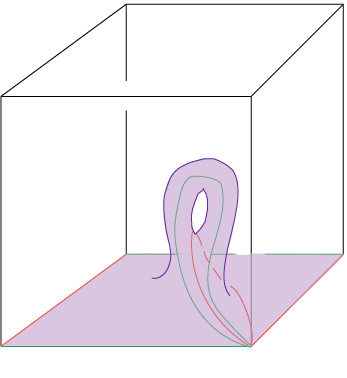
\includegraphics[width=.6\linewidth]{Wg2}
  \captionof{figure}{An embedding $W_{2} \hookrightarrow \TT^{3}$}
  \label{fig:test1}
\end{minipage}%
\begin{minipage}{.5\textwidth}
  \centering
  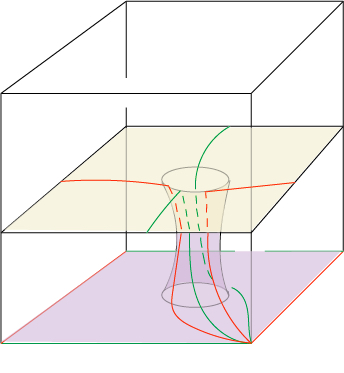
\includegraphics[width=.6\linewidth]{Wg1}
  \captionof{figure}{A different embedding $W_{2} \hookrightarrow \TT^{3}$}
  \label{fig:test2}
\end{minipage}
\end{figure}

The reason that these embeddings lie in different path components is because restricting each embedding to the $1-$skeleton, which are colored red and green in the figures, yield different elements of $(\pi_{1}\TT^{3})^{4}.$



Next, we identify a weak homotopy equivalence between ${\sf Imm}(W_{g}, M)$ and mapping spaces which will have computable homotopy groups.


%%%%%%%%%%%% STRUCTURE OF ARGUMENT %%%%%%%%%%%%%%%
\section{A Homotopy Equivalence Between Bundle Injections and Mapping Spaces} 
Recall that by the Hirsch-Smale Theorem \ref{hst} we have that ${\sf Imm}(W_{g}, M)$ is weakly homotopy equivalent to ${\sf Imm^{f}}(W_{g}, M),$ the space of \textit{formal immersions} which we defined (Definition \ref{formalimmdef}) as fiberwise bundle injections between tangent bundles: 
\[
{\sf Imm^{f}}(W_{g}, M) := {\sf BunInj}(\tau_{W_{g}}, \tau_{M})~.
\]
Under our assumption that $M$ is parallelizable, we have that there is a homeomorphism 
\begin{equation} \label{eq1new}
{\sf Imm^{f}}(W_{g}, M) := {\sf BunInj}(\tau_{W_{g}}, \tau_{M}) \xra{\approx} {\sf BunInj}(\tau_{W_{g}}, \epsilon_{M}^{n})
\end{equation}
from a choice of trivialization of the tangent bundle of $M.$


\begin{convention} \label{cov1}
Recall from Convention \ref{cccc} that we endow ${\sf Map}(X, Y)$ with the appropriate topology depending on whether or not $X$ and $Y$ are smooth manifolds. Natural subspaces such as immersions, ${\sf Imm}(W_{g}, M) \hookrightarrow {\sf Imm^{f}}(W_{g}, M) \subset {\sf Map}(\sT W_{g}, \sT M),$ or based maps ${\sf Map}_{\ast}(X, Y) \subset {\sf Map}(X, Y),$ will be equipped with the subspace topology. Similarly, we equip both ${\sf BunInj}(\tau_{W_{g}}, \tau_{M}) \subset {\sf Map}(TW_{g}, TM)$ and ${\sf BunInj}_{/W}(E \rightarrow W, E' \rightarrow W) \subset {\sf Map}(E, E')$ with the appropriate subspace topology.
\end{convention}




\begin{lemma} \label{lem.homeo}
There is a homeomorphism between spaces 
\[
h: {\sf Map^{smooth}}(W_{g}, M) \times {\sf BunInj}_{/W_{g}}(\tau_{W_{g}}, \epsilon_{W_{g}}^{n}) \rightarrow {\sf BunInj}(\tau_{W_{g}}, \epsilon_{M}^{n})
\]
given by 
\[\left( (W_{g} \xra{f} M), \left(\begin{tikzcd}
TW_{g} \arrow[rd] \arrow[r, "F"]  & \RR^{n} \times W_{g} \arrow[d]\\
& W_{g}
\end{tikzcd} \right) \right)
\mapsto \left(
\begin{tikzcd}
TW_{g} \arrow[rd] \arrow[r, "F"] & \RR^{n} \times W_{g} \arrow[d]  \arrow[r, "id \times f"]& \RR^{n} \times M \arrow[d] \\
& W_{g} \arrow[r, "f"] & M
\end{tikzcd} \right)~.
\]
\end{lemma}

\begin{proof}
The map $h$ is continuous as it the composition of continuous maps with regard to the topologies in Convention \ref{cov1}.
We can define the inverse map as follows:
\[
h^{-1}\left(\begin{tikzcd}
TW_{g} \arrow[d] \arrow[r, "F"]  & \RR^{n} \times M \arrow[d]\\
W_{g} \arrow[r, "f"] & M
\end{tikzcd} \right) =
\left( (W_{g} \xra{f} M), \left(\begin{tikzcd}
TW_{g} \arrow[rd] \arrow[r, "\tilde{F}"]  & \RR^{n} \times W_{g} \arrow[d]\\
& W_{g}
\end{tikzcd} \right) \right)
\]
where for $v \in T_{x}W_{g}$ we have that $\tilde{F}(v, x) = (F_{x}(v), x) \in \RR^{n} \times W_{g}.$ 
This is again a continuous map and therefore $h$ is a homeomorphism.
\end{proof}


\begin{definition}
Given continuous maps $A \xra{f} C$ and $B \xra{g} C$ we defined the \bit{homotopy pullback} of these maps to be 
\[
A \times_{C}^{h} B := A \times_{C} C^{I} \times_{C} B = \{(a, \gamma, b): f(a) = \gamma(0), g(b) = \gamma(1) \}
\]
along with the projection maps:
\[
\xymatrix{
A \times_{C}^{h} B \ar[rr]^-{{\sf proj}_{B}} \ar[d]^-{{\sf proj}_{A}}
&&
B \ar[d]^-{g}
\\
A \ar[rr]^-{f}
&&
C~.
}
\]
In the case that $A = \ast$ and $f$ selects out the point $c_{0} \in C$, this homotopy pullback is the \bit{homotopy fiber} of $g$ over $c_{0}$ and we denote it as ${\sf hofib}_{c_{0}}(B \xra{g} C).$ 
\end{definition}

We will use properties of homotopy pullbacks frequently in this dissertation.

\begin{remark} \label{rem.hpull}
Recall that a homotopy commutative diagram
\[
\xymatrix{
D \ar[rr]^-{\varphi_{B}} \ar[d]^-{\varphi_{A}}
&&
B \ar[d]^-{g}
\\
A \ar[rr]^-{f}
&&
C~.
}
\]
is called a homotopy pullback diagram if the associated map $D \xra{\varphi} A \times_{C}^{h} B$ from Proposition \ref{diagram.to.map} is a homotopy equivalence.
This alternative definition of a homotopy pullback will often be much more convenient to work with.
\end{remark}


We will now discuss how one can think of the tangent bundle of $W_{g}$ as an element of ${\sf Map}(W_{g}, {\sf BO}(2)).$ Choose some embedding $e: W_{g} \hookrightarrow \RR^{N}$ so that $e(W_{g}) \subset \RR^{N}$ is a smooth submanifold. Then define the map 
\[
Te: W_{g} \rightarrow {\sf Gr}_{2}(N); \hspace{20pt} p \mapsto \big(T_{e(p)}e(W_{g}) \subset T_{e(p)}\RR^{N} = \RR^{N}\big)~.
\]
Then the map
\[
\tau_{W_{g}}: W_{g} \xra{Te} {\sf Gr}_{2}(N) \hookrightarrow {\sf Gr}_{2}(\infty) = {\sf BO}(2)
\]
describes an element in ${\sf Map}(W_{g}, {\sf BO}(2)).$ By the Whitney Embedding Theorem, this map $\tau_{W_{g}}$ is independent of the choice of embedding up to homotopy.

Therefore, it makes sense to consider the homotopy fiber of the map \[
{\sf Map}(W_{g}, {\sf Gr_{2}}(n)) \xra{\gamma_{2} \circ -} {\sf Map}(W_{g}, {\sf BO}(2))\] over $\tau_{W_{g}}$ where $\gamma_{2}$ is the natural inclusion $\Gr_2(n) \hookrightarrow \Gr_{2}(\infty) = {\sf BO}(2).$ We take this homotopy fiber as the definition of ${\sf Map}_{/{\sf BO}(2)}(W_{g}, \Gr_2(n)),$ i.e.
\[
{\sf Map}_{/{\sf BO}(2)}(W_{g}, \Gr_2(n)) := {\sf hofib}_{\tau_{W_{g}}}({\sf Map}(W_{g}, \Gr_{2}(n)) \xra{\gamma_{2} \circ } {\sf Map}(W_{g}, {\sf BO}(2))).
\]





\begin{observation} \label{obsl0}
Applying Equation (\ref{l0m}) to $W_{g},$ we have the canonical homotopy-equivalence:  
\[
{\sf BunInj}_{/W_{g}}(\tau_{W_{g}}, \epsilon_{W_{g}}^{n}) \rightarrow {\sf Map}_{/{\sf BO}(2)}(W_{g}, \Gr_2(n))~.
\]
Specifying an orientation $\sigma$ on $W_{g},$ Equation (\ref{l1m}) give the canonical homotopy-equivalence:
\[
{\sf BunInj}_{/W_{g}}(\tau_{W_{g}}, \epsilon_{W_{g}}^{n}) \rightarrow {\sf Map}_{/{\sf BSO}(2)}(W_{g}, \Gr_2^{\sf or}(n))~.
\]
\end{observation}


\begin{remark} \label{rrr}
Recall that by the Smooth Approximation Theorem \cite{Woc} there is a homotopy equivalence ${\sf Map^{smooth}}(X, Y) \simeq {\sf Map}(X, Y).$
\end{remark}

To summarize what we have done in this section, we have shown that there is a weak homotopy equivalence 
\begin{equation} \label{heeq}
{\sf Imm}(W_{g}, M) \xra[\simeq]{\text{Theorem }\ref{hst}} {\sf Imm^{f}}(W_{g}, M) \xra[\simeq]{\text{Lemma }\ref{lem.homeo}} {\sf Map^{smooth}}(W_{g}, M) \times {\sf BunInj}_{/W_{g}}(\tau_{W_{g}}, \epsilon_{W_{g}}^{n}) 
\end{equation}
\[
\xra[\simeq]{\text{Remark } \ref{rrr} \times \text{Observation }\ref{obsl0}} {\sf Map}(W_{g}, M) \times {\sf Map}_{/{\sf BSO}(2)}(W_{g}, \Gr_2^{\sf or}(n)).
\]

We will examine the homotopy groups of each of these factors in later sections. Our method of attack will be to first calculate $\pi_{k}{\sf Map}(W_{g}, Z)$ for $Z$ a general based topological space. Then we identify a homotopy equivalence ${\sf Map}_{/{\sf BSO}(2)}(W_{g}, \Gr_2^{\sf or}(n)) \simeq {\sf Map}(W_{g}, \sV_{2}(n)).$









\section{Homotopy Groups of Mapping Spaces}
In this section we relate the homotopy groups of ${\sf Map}(W_{g}, Z)$ to the homotopy groups of $Z,$ where $Z$ is a based, path-connected topological space. We begin with the homotopy groups $\pi_{k}{\sf Map}(W_{g}, Z)$ for $k > 0$, and deal with the set of path components, $\pi_{0}{\sf Map}(W_{g}, Z),$ in the next section.

\begin{lemma} \label{moreuniqlemma1}
For based topological spaces $(X, x_{0}), (Y, y_{0})$ we have that the following spaces are homotopy equivalent:
\[
{\sf Map}(X, \Omega_{y_{0}}Y) \simeq {\sf Map}_{\ast}(X, \Omega_{y_{0}}Y) \times \Omega_{y_{0}}Y
\]
where we take the constant map $S^{1} \rightarrow Y$ at $y_{0}$ to be the base point of $\Omega_{y_{0}}Y.$
\end{lemma}
\begin{proof}
Consider the map 
\[
F \colon {\sf Map}(X, \Omega_{y_{0}}Y) \longrightarrow {\sf Map}_{\ast}(X, \Omega_{y_{0}}Y) \times \Omega_{y_{0}}Y; \hspace{15pt} f \mapsto ((f(x_{0}))^{\ast}f, f(x_{0}))
\]
where $(f(x_{0}))^{\ast} \in \Omega_{y_{0}}Y$ is the loop $f(x_{0})$ with the opposite orientation.
Now consider the map
\[
G \colon {\sf Map}_{\ast}(X, \Omega_{y_{0}}Y) \times \Omega_{y_{0}}Y \longrightarrow {\sf Map}(X, \Omega_{y_{0}}Y); \hspace{15pt} (g, \gamma) \mapsto \gamma g~.
\]
We will show that $F \circ G \simeq \id_{({\sf Map}_{\ast}(X, \Omega_{y_{0}}Y) \times \Omega_{y_{0}}Y)}$ and $G \circ F \simeq \id_{{\sf Map}(X, \Omega_{y_{0}}Y)}.$ First
\[
(F \circ G)(g, \gamma) = ((\gamma g(x_{0}))^{\ast}(\gamma g), \gamma g(x_{0})) = ((\gamma \gamma_{y_{0}})^{\ast}(\gamma g), \gamma \gamma_{y_{0}}) = (\gamma_{y_{0}}^{\ast} \gamma^{\ast} \gamma g, \gamma \gamma_{y_{0}}) \simeq (g, \gamma)
\]
where the last homotopy is due to $\gamma \gamma_{y_{0}} \simeq \gamma$ and $\gamma^{\ast} \gamma \simeq \gamma_{y_{0}}.$ Lastly,
\[
(G \circ F)(f) = f(x_{0})(f(x_{0}))^{\ast}f \simeq f
\]
showing that $F$ and $G$ are homotopy inverses proving our claim.
\end{proof}

\begin{observation} \label{oooo}
Note that the argument above can also be used to show that for a based space $(X, x_{0})$ and a topological group $G,$ that 
\[
{\sf Map}(X, G) \simeq {\sf Map}_{\ast}(X, G) \times G~.
\]
\end{observation}

\begin{lemma} \label{moreuniqlemma2}
For based topological spaces $(X, x_{0}), (Y, y_{0})$ in which $x_{0} \in X$ has a neighborhood that deformation retracts onto $\{x_{0}\},$ we have that for $k \geq 1$ there is an isomorphism of groups: 
\[
\pi_{k}{\sf Map}(X, Y) \cong \pi_{k}{\sf Map}_{\ast}(X, Y) \times \pi_{k}Y~,
\]
where we take the constant map at $y_{0}$ to be the base point of ${\sf Map}_{\ast}(X, Y)$ and ${\sf Map}(X, Y).$
\end{lemma}
\begin{proof}
Consider the following pullback diagram, 
\begin{equation} \label{sumdiag}
\xymatrix{
{\sf Map}_{\ast}(X, Y) \ar[rr]^-{} \ar[d]^-{}
&&
{\sf Map}(X, Y) \ar[d]^-{ev_{x_{0}}}
\\
\ast \ar[rr]^-{\langle y_{0} \rangle} 
&&
Y ~.
}
\end{equation}
The assumption ensures $\ast \xra{x_{0}} X$ is a cofibration. Therefore, $ev_{x_{0}}$ is a fibration and thus (\ref{sumdiag}) is a homotopy pullback.
So from (\ref{sumdiag}) we get the associated long exact sequence on homotopy groups:
\[
\xymatrix{
\hdots \ar[r]^-{}
&
\pi_{k + 1}{\sf Map}_{\ast}(X, Y) \ar[rr]^-{} 
&&
\pi_{k + 1}{\sf Map}(X, Y) \ar[rr]^-{}
&&
\pi_{k + 1}Y \ar[dllll]^{\partial_{k}}
&
\\
&
\pi_{k}{\sf Map}_{\ast}(X, Y) \ar[rr]^-{} 
&&
\pi_{k}{\sf Map}(X, Y) \ar[rr]^-{}
&&
\pi_{k}Y \ar[r]^-{}
&
\hdots 
}
\]
Note that we have a section of spaces
\[
s:Y \rightarrow {\sf Map}(X, Y); \hspace{15 pt} y \mapsto ( {\sf const}_{y}: X \rightarrow Y)~,
\] that is $ev_{x_{0}} \circ s = id_{Y}.$ This induces a section of homotopy groups $s^{\ast}: \pi_{k}Y \rightarrow \pi_{k}{\sf Map}(X, Y)$ and implies that $ev_{x_{0}}^{\ast}$ will be surjective and therefore all boundary maps are trivial, $\partial_{k} = 0.$ 
Therefore our long exact sequence is divided into short exact sequences of the form:
\begin{equation} \label{moruniq}
0 \longrightarrow \pi_{k}{\sf Map}_{\ast}(X, Y) \longrightarrow \pi_{k}{\sf Map}(X, Y) \longrightarrow \pi_{k}Y \longrightarrow 0~.
\end{equation} 
For $k \geq 2,$ the existence of $s^{\ast}$ and the Splitting Lemma immediately implies that (\ref{moruniq}) splits:
\[
\pi_{k}{\sf Map}(X, Y) \cong \pi_{k}{\sf Map}_{\ast}(X, Y) \times \pi_{k}Y ~.
\]
For $k = 1,$ we can rewrite (\ref{moruniq}) as 
\[
0 \longrightarrow \pi_{0}{\sf Map}_{\ast}(X, \Omega_{y_{0}}Y) \longrightarrow \pi_{0}{\sf Map}(X, \Omega_{y_{0}}Y) \longrightarrow \pi_{0}\Omega_{y_{0}}Y \longrightarrow 0
\]
and Lemma \ref{moreuniqlemma1} implies that this short exact sequence is split as a product as well. Therefore for $k \geq 1$ we have that 
\[
\pi_{k}{\sf Map}(X, Y) \cong \pi_{k}{\sf Map}_{\ast}(X, Y) \times \pi_{k}Y~.
\]
\end{proof}


\begin{remark}
Dual to the definition of homotopy pullback, there is the notion of \textbf{homotopy pushout} for which we gave an explicit definition in Chapter \ref{CH:B}. One property we will use frequently is that if the following diagram is a pushout:
\[
\xymatrix{
W \ar[rr]^-{f} \ar[d]^-{g}
&&
X \ar[d]^{j}
\\
Y \ar[rr]^{k}
&&
Z
}
\]
and either $f$ or $g$ are cofibrations, then it also realizes a homotopy pushout diagram.
\end{remark}

\subsection{Geometric Crux}
The following geometric argument is the insight which enabled us to consider homotopy groups of ${\sf Imm}(W_{g}, M)$ for arbitrary $g \geq 0.$ This extends Smale's result \cite{Sm3} which identifies the homotopy groups for genus 0, i.e. $\pi_{k}{\sf Imm}(S^{2}, M).$ We start by recalling the definitions of some basic operations on pointed topological spaces.

\begin{definition}
Let $(Z, z_{0})$ be a pointed topological space. The \textit{reduced suspension} of $Z$ is defined to be 
\[
\Sigma Z := (Z \times I)/ \Big((Z \times \{0\}) \cup (\{z_{0}\} \times I) \cup (Z \times \{1\}) \Big)
\] 
where $I = [0, 1].$
\end{definition}

\begin{definition}
Given pointed topological spaces $(Z, z_{0})$ and $(W, w_{0}),$ the wedge sum of $Z$ and $W$ is defined as 
\[
Z \vee W := (Z \sqcup W)/(\{z_{0}\} \sim \{w_{0}\})~.
\]
We denote the iterated wedge sum of $(Z, z_{0})$ with itself $n-$times as $Z^{\vee n}.$
\end{definition}

\begin{observation} \label{ooooo}
Consider the following pushout diagram,
\begin{equation}\label{classicpushout}
\xymatrix{
\partial \DD^{2} = S^{1} \ar[rr]^-{c} \ar[d]^-{i}
&&
(S^{1})^{\vee 2g} \ar[d]^-{}
\\
\DD^{2} \ar[rr]^-{} 
&&
W_{g}~,
}
\end{equation}
where $[c] \in \pi_{1}((S^{1})^{\vee 2g})$ is the product of commutators $a_{1}b_{1}a_{1}^{-1}b_{1}^{-1} \hdots a_{n}b_{n}a_{n}^{-1}b_{n}^{-1}.$ As the inclusion $i: \partial \DD^{2} \rightarrow \DD^{2}$ is a cofibration, the diagram is a homotopy pushout diagram.
\end{observation}




\begin{lemma} \label{geom.crux}
There is a homotopy equivalence between spaces,
\[
\Sigma W_{g} \simeq \Sigma \big( S^{2} \vee (S^{1})^{\vee 2g}\big)~. 
\]
\end{lemma}
\begin{proof}
Taking the reduced suspension of all spaces and maps in diagram (\ref{classicpushout}) results in the homotopy pushout diagram:
\begin{equation} \label{anothalabel}
\xymatrix{
\Sigma S^{1} \simeq S^{2} \ar[rr]^-{\Sigma c} \ar[d]^-{\Sigma i}
&&
\Sigma (S^{1})^{\vee 2g} \ar[d]^-{}
\\
\Sigma \DD^{2} \ar[rr]^-{} 
&&
\Sigma W_{g}~.
}
\end{equation} 
Note that the homomorphism 
\[
\langle a_{1}, b_{1}, \hdots, a_{n}, b_{n} \rangle = \pi_{1}\big((S^{1})^{\vee 2g}\big) \xra{\Sigma} \pi_{2}\big(\Sigma(S^{1})^{\vee 2g}\big); \hspace{20pt}  [\gamma] \mapsto [\Sigma \gamma]
\]
must factor through the abelianization of $\pi_{1}\big((S^{1})^{\vee 2g}\big)$ since $\pi_{2}\big(\Sigma(S^{1})^{\vee 2g}\big)$ is abelian. That is, there exists a unique map such that the following diagram commutes,
\[
\begin{tikzcd}
\langle a_{1}, b_{1}, \hdots, a_{n}, b_{n} \rangle = \pi_{1}\big((S^{1})^{\vee 2g}\big) \arrow[r, "q"] \arrow[rd, "\Sigma"]
&  \pi_{1}\big((S^{1})^{\vee 2g}\big)_{Ab} \cong \ZZ^{2g} \arrow[d, "!"] \\
&  \pi_{2}\big(\Sigma(S^{1})^{\vee 2g}\big)
\end{tikzcd}
\]
where the map $q$ is the canonical quotient map. Now clearly $[c] = a_{1}b_{1}a_{1}^{-1}b_{1}^{-1} \hdots a_{n}b_{n}a_{n}^{-1}b_{n}^{-1}$ is in the kernel of $q$ and therefore it is also in the kernel of $\Sigma,$ i.e. $\Sigma c$ is homotopic to the constant map at the basepoint.
Now in (\ref{anothalabel}), we have identified 
\[
\Sigma W_{g} = {\sf hopush} \left( \begin{tikzcd}
\Sigma S^{1} \arrow[r, "\Sigma c"] \arrow[d, "\Sigma i"] & \Sigma\big( (S^{1})^{\vee 2g} \big) \\
\Sigma \DD^{2}
\end{tikzcd} \right).
\] As this is a homotopy pushout, we may replace any spaces with homotopy equivalent spaces and any maps with homotopic maps and the resulting homotopy pushout will be homotopy equivalent. 
Therefore 
\[
\Sigma W_{g} = {\sf hopush} \left( \begin{tikzcd}
\Sigma S^{1} \arrow[r, "\Sigma c"] \arrow[d, "\Sigma i"] & \Sigma\big( (S^{1})^{\vee 2g} \big) \\
\Sigma \DD^{2}
\end{tikzcd} \right) \simeq 
{\sf hopush} \left( \begin{tikzcd}
\Sigma S^{1} \arrow[r, "{\sf const}_{\ast}"] \arrow[d, "!"] & \Sigma\big( (S^{1})^{\vee 2g} \big) \\
\ast
\end{tikzcd} \right) \simeq
\] 
\[ 
\Sigma \left( {\sf hopush} \left( \begin{tikzcd}
S^{1} \arrow[r, "{\sf const}_{\ast}"] \arrow[d, "!"] & \big((S^{1})^{\vee 2g} \big) \\
\ast
\end{tikzcd} \right) \right) \simeq
\]
\[
\Sigma \left(\ast \cup_{S^{1} \times 0} S^{1} \times I \cup_{S^{1} \times 1} \big( (S^{1})^{\vee 2g} \big)\right) \simeq \Sigma \big( S^{2} \vee (S^{1})^{\vee 2g}\big)~.
\]
\end{proof}



\begin{prop} \label{prop.hom}
Let $Z$ be based, path-connected topological space. Then consider the based space of all continuous maps, ${\sf Map}(W_{g}, Z),$ with the constant map ${\sf const}_{z_{0}}$
serving as its base point. Then, for $k \geq 1,$ we have the following isomorphism of groups:
\[
\pi_{k}{\sf Map}(W_{g}, Z) \cong \pi_{k}Z \times (\pi_{k + 1}Z)^{2g} \times \pi_{k + 2}Z.
\]
\end{prop}
\begin{proof}
Consider the following homotopy pushout diagram, 
\[
\xymatrix{
(S^{1})^{\vee 2g} \ar[rr]^-{i} \ar[d]^-{}
&&
W_{g} \ar[d]^-{}
\\
\ast \ar[rr]^-{} 
&&
\DD^{2}/\partial \DD^{2} \cong S^{2}
}
\]
where the map $i: (S^{1})^{\vee 2g} \rightarrow W_{g},$ the inclusion of the $1$-skeleton into $W_{g},$ is a cofibration. We may then apply ${\sf Map}_{\ast}(-, Z)$ to this diagram to get the following homotopy pullback diagram,
\begin{equation} \label{beforepuppseq}
\xymatrix{
{\sf Map}_{\ast}(S^{2}, Z) \cong \Omega^{2}Z \ar[rr]^-{} \ar[d]^-{}
&&
{\sf Map}_{\ast}(W_{g}, Z) \ar[d]^-{}
\\
\ast \ar[rr]^-{} 
&&
{\sf Map}_{\ast}((S^{1})^{\vee 2g}, Z) \cong (\Omega Z)^{2g}~.
}
\end{equation}
The Puppe sequence, see Theorem 11.39 of \cite{Rot}, then implies that following is also a homotopy pullback diagram,
\begin{equation}\label{puppseq}
\xymatrix{
\Omega( \Omega^{2}Z) \ar[rr]^-{} \ar[d]^-{}
&&
\Omega {\sf Map}_{\ast}(W_{g}, Z) \cong {\sf Map}_{\ast}(\Sigma W_{g}, Z) \ar[d]^-{}
\\
\ast \ar[rr]^-{} 
&&
\Omega (\Omega Z)^{2g}~.
}
\end{equation}
Now from Lemma \ref{geom.crux} we have that $\Sigma W_{g} \simeq \Sigma(S^{2} \vee (S^{1})^{2g})$ and so we have the following homotopy equivalence: 
\[
{\sf Map}_{\ast}(\Sigma W_{g}, Z) \simeq {\sf Map}_{\ast}(\Sigma(S^{2} \vee (S^{1})^{2g}), Z) \simeq \Omega {\sf Map}_{\ast}(S^{2} \vee (S^{1})^{2g}, Z) \simeq \Omega(\Omega^{2}Z \times (\Omega Z)^{2g})~.
\]
This shows that the homotopy pullback above splits. So we have that 
\begin{equation} \label{eeee}
\Omega {\sf Map}_{\ast}(W_{g}, Z) \simeq \Omega( \Omega^{2}Z) \times \Omega (\Omega Z)^{2g}~.
\end{equation}
Therefore for $j \geq 0,$ 
\[
\pi_{j} \Omega {\sf Map}_{\ast}(W_{g}, Z)  \cong \pi_{j + 1}{\sf Map}_{\ast}(W_{g}, Z) \cong \pi_{j+ 3}Z \times (\pi_{j + 2}Z)^{2g} \cong \pi_{j}\Omega( \Omega^{2}Z) \times \pi_{j}\Omega (\Omega Z)^{2g}~.
\]
So after relabeling $k = j + 1$, for $k \geq 1,$  
\begin{equation} \label{e4uni}
\pi_{k}{\sf Map}_{\ast}(W_{g}, Z) \cong  (\pi_{k + 1}Z)^{2g} \times \pi_{k + 2}Z~.
\end{equation} 
By equation (\ref{e4uni}) and Lemma \ref{moreuniqlemma2} we have shown that there is the following isomorphism for $k \geq 1:$
\[
\pi_{k}{\sf Map}(W_{g}, Z) \cong \pi_{k}Z  \times  \pi_{k}{\sf Map}_{\ast}(W_{g}, Z) \cong \pi_{k}Z  \times (\pi_{k + 1}Z)^{2g} \times \pi_{k + 2}Z~.
\]
\end{proof}







\section{Connected Components of Mapping Spaces} \label{sec.connectedcomponents}
We will now examine the set $\pi_{0}{\sf Map}(W_{g}, Z)$ again considering $Z$ to be a based, path-connected, topological space. We first record the following Lemma which is proven in \cite{MoreMay}.

\begin{remark} \label{rm}
Given a based map $f: (X, x_{0}) \longrightarrow (Z, z_{0})$ and a loop $\gamma \in \pi_{1}Z,$ there is a homotopy $H: X \times I \longrightarrow Z$ such that $H_{0} = H|_{X \times \{0\}} = f$ and $H|_{\{x_{0}\} \times I} = \gamma.$ The existence of such a homotopy is due to the Covering Homotopy and Extension Property, which also can be used to show $[H_{1}]$ only depends on $[\gamma]$ and $[f].$
\end{remark}
\begin{lemma} \label{lem.pi1quot}
For $(X, x_{0})$ a based, path-connected, CW complex and $(Z, z_{0})$ a based, path-connected space there is a left action $\pi_{1}(Z; z_{0}) \curvearrowright \pi_{0}{\sf Map}_{\ast}(X, Z)$
defined by
\begin{equation} \label{anotheraction}
[\omega] \cdot [f] := H_{1}
\end{equation}
where $H_{t}$ is the homotopy from Remark \ref{rm}.
The natural map $\pi_{0}{\sf Map}_{\ast}(X, Z) \longrightarrow \pi_{0}{\sf Map}(X, Z)$ induces a bijection from the quotient
\[
\pi_{0}{\sf Map}_{\ast}(X, Z)/\pi_{1}(Z; z_{0}) \cong \pi_{0}{\sf Map}(X, Z)~.
\] 
\end{lemma}


If we take $X = S^{n}$ then the action from Lemma \ref{lem.pi1quot} becomes an action of $\pi_{1}Z$ on $\pi_{n}Z.$
\begin{definition}
If the action (\ref{anotheraction}) $\pi_{n}Z \simeq \pi_{0}{\sf Map}_{\ast}(S^{n}, Z) \curvearrowleft \pi_{1}(Z; z_{0})$ is trivial for all $n \geq 1,$ then the space $Z$ is called \textit{simple}. 
\end{definition}

For a simple space we immediately get the following Corollary of Lemma \ref{lem.pi1quot} .
\begin{cor}\label{cor.simple}
For $(Z, z_{0})$ a based, path-connected, simple space there is a bijection
\[
\pi_{0}{\sf Map}_{\ast}(W_{g}, Z) \cong \pi_{0}{\sf Map}(W_{g}, Z)~.
\]
\end{cor}

This will help us relate path components of unbased maps to those of based maps, under the assumption that our space $Z$ is simple. In Chapter \ref{CH:B}  we recorded some properties of simple spaces and justifications for why some of the spaces we are concerned with are simple.
We now work to identify $\pi_{0}{\sf Map}_{\ast}(W_{g}, Z),$ and we will start by examining a particular group action of $\pi_{2}Z$ on $\pi_{0}{\sf Map}_{\ast}(W_{g}, Z).$

First consider the following collapse map:
\[
\xymatrix{
\DD^{2} \ar[rr]^-{collapse}
&&
S^{2} \vee \DD^{2} 
\\
\partial \DD^{2} \ar[u]^-{i} \ar[rr]^-{\id_{\partial \DD^{2}}}
&&
\partial \DD^{2} \ar[u]^-{i}
}
\]
which collapses a circle lying completely in the interior of $\DD^{2}$ except at the basepoint. See Figure \ref{f} below. This induces a map between diagrams:
\[
\xymatrix{
\DD^{2} \ar[d]^-{collapse}
&&
\partial \DD^{2} \ar[ll]^-{i} \ar[rr]^-{c} \ar[d]^-{\id_{\partial \DD^{2}}}
&&
sk_{1} \ar[d]^-{\id_{sk_{1}}}
\\
S^{2} \vee \DD^{2}  
&&
\partial \DD^{2} \ar[ll]^-{i} \ar[rr]^-{c}
&&
sk_{1}
}
\]
which then induces the map between pushouts:
\begin{equation}
W_{g} \xra{collapse} W_{g} \vee S^{2}~.
\end{equation}
Note that because the circle we collapse along in $\DD^{2} \xra{collapse} S^{2} \vee \DD^{2}$ is contained in the interior of $\DD^{2}$ except at the basepoint, the map $W_{g} \xra{collapse} 
W_{g} \vee S^{2}$ does not alter the 1-skeleton of $W_{g}$.



\begin{figure}[h]
\centering
\includegraphics[width=0.5\textwidth]{collapse}
\caption{The collapse map, $\DD^{2} \xra{collapse} S^{2} \vee \DD^{2}~.$}\label{f}
\end{figure}


\begin{lemma}
Take $(Z, z_{0})$ to be a based, path-connected, topological space. Now consider the map: 
\[
\pi_{2}Z \times \pi_{0}{\sf Map}_{\ast}(W_{g}, Z) \longrightarrow \pi_{0}{\sf Map}_{\ast}(W_{g}, Z)\]
\begin{equation} \label{action}([\omega: S^{2} \rightarrow Z], [f: W_{g} \rightarrow Z]) \mapsto [W_{g} \xra{collapse} S^{2} \vee W_{g} \xra{\omega \vee f} Z] =: [\omega] \cdot [f]~. \end{equation}
This map defines a left group action of $\pi_{2}Z$ on the set $\pi_{0}{\sf Map}_{\ast}(W_{g}, Z).$
\end{lemma}
\begin{proof}
Recall from Remark \ref{homprod} that the addition rule of $\pi_{2}Z$ can be described as 
\[
[S^{2} \xra{\omega_{2}} Z] + [S^{2} \xra{\omega_{1}} Z] = [S^{2} \xra{collapse_{S^{1}}} S^{2} \vee S^{2} \xra{\omega_{2} \vee \omega_{1}} Z]
\] where the map $S^{2} \xra{collapse_{S^{1}}} S^{2} \vee S^{2}$ collapses some fixed great circle containing the basepoint. Then we have that 
\[
[\omega_{2}] \cdot ([\omega_{1}] \cdot [f]) = [\omega_{2}] \cdot [W_{g} \xra{collapse} S^{2} \vee W_{g} \xra{\omega_{1} \vee f} Z] = [W_{g} \xra{collapse} S^{2} \vee W_{g} \xra{\omega_{2} \vee (\omega_{1} \cdot f)} Z]
\]
\[
= [W_{g} \xra{collapse} S^{2} \vee W_{g} \xra{\omega_{2} \vee collapse} S^{2} \vee (S^{2} \vee W_{g}) \xra{\omega_{2} \vee (\omega_{1} \vee f)} Z]
\]
\[
= [W_{g} \xra{collapse} S^{2} \vee W_{g} \xra{collapse_{S^{1}} \vee id} S^{2} \vee S^{2} \vee W_{g} \xra{\omega_{2} \vee \omega_{1} \vee f}] = ([\omega_{2}] + [\omega_{1}]) \cdot [f]~.
\]
Next, the identity element of $\pi_{2}Z$ is $[e] = [S^{2} \xra{{\sf const}_{z_{0}}} Z],$ the constant map at the base point. Then
\[
[e] \cdot [f] = [W_{g} \xra{collapse} S^{2} \vee W_{g} \xra{{\sf const}_{z_{0}} \vee f} Z] = [W_{g} \xra{f} Z] = [f]~. 
\] 
Therefore the map (\ref{action}) does indeed define a group action.
\end{proof}

Consider the set 
\[
(\pi_{1}Z)^{2g}_{\rm Com} := \{ ([\alpha_{1}], [\beta_{1}], \hdots [\alpha_{g}], [\beta_{g}]) \in (\pi_{1}Z)^{2g} : [\alpha_{1}, \beta_{1}][\alpha_{2}, \beta_{2}]\hdots[\alpha_{g}, \beta_{g}] = [e] \} \subset (\pi_{1}Z)^{2g}
\]
where $[\alpha_{1}, \beta_{i}] = \alpha_{i}\beta_{i}\alpha_{i}^{-1}\beta_{i}^{-1}$ is the commutator of $\alpha_{i}$ and $\beta_{i}$. Now consider the map
\begin{equation}\label{e1unii}
\Phi: \pi_{0}{\sf Map}_{\ast}(W_{g}, Z)/\pi_{2}Z \longrightarrow (\pi_{1}Z)^{2g}_{\rm Com}
\end{equation}
\[
[W_{g} \xra{f} Z] \mapsto ([f|_{a_{1}}], [f|_{b_{1}}], \hdots, [f|_{a_{g}}], [f|b_{g}])
\]
where $a_{i}, b_{i}$ are the 1-cells of $W_{g}.$ 
\newline \newline
Let $(Z, z_{0})$ be a based space. Restricting a based map $W_{g} \longrightarrow Z$ along its one skeleton, $(S^{1})^{\vee 2g} \cong sk_{1} \hookrightarrow W_{g} \longrightarrow Z,$ results in a map ${\sf Map}_{\ast}(W_{g}, Z) \rightarrow {\sf Map}_{\ast}((S^{1})^{\vee 2g}, Z) \cong (\Omega Z)^{2g}.$ Applying $\pi_{0}$ to this map results in the map 
\[
\w{\Phi}: \pi_{0}{\sf Map}_{\ast}(W_{g}, Z) \longrightarrow (\pi_{1}Z)^{2g}~.
\]

\begin{observation}
The map $\w{\Phi}$ factors
\[
\begin{tikzcd}
\pi_{0}{\sf Map}_{\ast}(W_{g}, Z) \arrow[d, "q"] \arrow[rr, "\w{\Phi}"] && (\pi_{1}Z)^{2g}     \\
\pi_{0}{\sf Map}_{\ast}(W_{g}, Z)/\pi_{2}Z \arrow[rr, "\Phi"] && \arrow[u, "inc."]   (\pi_{1}Z)^{2g}_{\rm Com}~.
\end{tikzcd}
\]

Indeed, for a based map $f: W_{g} \longrightarrow Z,$ the commutative diagram:
\[
\begin{tikzcd}
\partial \DD^{2 }\arrow[d, "i"] \arrow[rr, "c"] && sk_{1} \arrow[d, ""] &&  \\
\DD^{2} \arrow[rr, ""] &&   W_{g} \arrow[rr, "f"] && Z 
\end{tikzcd}
\]
reveals that $\w{\Phi}([f]) \in  (\pi_{1}Z)^{2g}_{\rm Com}.$ 
Furthermore, the map (\ref{e1unii}) is well defined. Indeed, $W_{g}$ is obtained by gluing the boundary of a 2-disk to the 1-skeleton by $a_{1}b_{1}a_{1}^{-1}b_{1}^{-1}\hdots a_{g}b_{g}a_{g}^{-1}b_{g}^{-1}.$ So given a continuous based map, $f\colon W_{g} \rightarrow Z,$ restricting to the 1-skeleton results in based loops $f|_{a_{1}}, f|_{b_{1}}, \hdots f|_{a_{g}}, f|_{b_{g}}$ in $Z$ for which $f|_{a_{1}}f|_{b_{1}}f|_{a_{1}}^{-1}f|_{b_{1}}^{-1}\hdots f|_{a_{g}}f|_{b_{g}}f|_{a_{g}}^{-1}f|_{b_{g}}^{-1}$ is contractible. 
Suppose $[f] = [\omega] \cdot [g],$ i.e. $[f]$ and $[g]$ are in the same orbit of (\ref{action}). As the disk we collapse along in our action does not intersect the 1-skeleton on $W_{g}$ other than at the base point, restricting $f$ and $g$ to the 1-skeleton will be equal up to homotopy. That is $[f|_{a_{1}}] = [g|_{a_{1}}], \hdots, [f|_{b_{g}}] = [g|_{b_{g}}],$ and so the map (\ref{e1unii}) is well defined.


\end{observation}


\begin{lemma} 
Let $(Z, z_{0})$ be a based space. The map $\Phi$ from equation (\ref{e1unii}) is surjective. % so for each $([\alpha_{1}], [\beta_{1}], \hdots [\alpha_{g}], [\beta_{g}]) \in (\pi_{1}Z)^{2g}_{Com}$ there is some $f \in {\sf Map}_{\ast}(W_{g}, Z)$ for which 
%\[
%\w{\Phi}^{-1}([\alpha_{1}], [\beta_{1}], \hdots [\alpha_{g}], [\beta_{g}]) \ni [f]~.
%\] 
\end{lemma}
\begin{proof}
To see that (\ref{e1unii}) is surjective take any $([\alpha_{1}], [\beta_{1}], \hdots [\alpha_{g}], [\beta_{g}]) \in (\pi_{1}Z)^{2g}$ for which 
\[
[\alpha_{1}, \beta_{1}][\alpha_{2}, \beta_{2}]\hdots[\alpha_{g}, \beta_{g}] = [e]~.
\]
We can construct $[\w f] \in \pi_{0}{\sf Map}_{\ast}(W_{g}, Z)$ as follows:
$\w f$ maps the 0-cell of $W_{g}$ to the base point of $Z.$ For the 1-skeleton of $W_{g}$ we have $\w f(a_{1}) = \alpha_{i}, \w f(b_{i}) = \beta_{i}.$ And finally the 2-cell of $W_{g}$ is mapped to the disk bounded by $[\alpha_{1}, \beta_{1}][\alpha_{2}, \beta_{2}]\hdots[\alpha_{g}, \beta_{g}].$ Then \[
(\Phi \circ q)([\w f]) = [\alpha_{1}, \beta_{1}][\alpha_{2}, \beta_{2}]\hdots[\alpha_{g}, \beta_{g}], 
\]
which shows $\Phi \circ q$ is surjective, this implies that $\Phi$ is also surjective.
\end{proof}


\begin{lemma} \label{rep}
Fix some $([\bar{\alpha}] ,[\bar{\beta}]) := ([\alpha_{1}], [\beta_{1}], \hdots [\alpha_{g}], [\beta_{g}]) \in (\pi_{1}Z)^{2g}_{\rm Com},$ and fix some $f \in {\sf Map}_{\ast}(W_{g}, Z)$ such that $\w{\Phi}([f]) = ([\bar{\alpha}] ,[\bar{\beta}]).$
Let $[g] \in \w{\Phi}^{-1}([\bar{\alpha}] ,[\bar{\beta}]).$ Then there is some representative $g_{rep} \in [g]$ such that $g_{rep}|_{sk_{1}} = f|_{sk_{1}}.$
\end{lemma}
\begin{proof}
The inclusion $sk_{1} \hookrightarrow W_{g}$ is a cofibration. Therefore, the restriction map 
\[
R: {\sf Map}_{\ast}(W_{g}, Z) \rightarrow {\sf Map}_{\ast}(sk_{1}, Z); \hspace{15pt} g \mapsto g|_{sk_{1}}
\]
is a fibration. There is a homotopy $\gamma$ in  ${\sf Map}_{\ast}(sk_{1}, Z)$ from $g|_{sk_{1}}$ to $f|_{sk_{1}}.$ Consider the following diagram:
\[
\xymatrix{
\{0\} \ar[rr]^-{<g>} \ar[d]^-{}
&&
{\sf Map}_{\ast}(W_{g}, Z) \ar[d]^-{R}
\\
I \ar[rr]^-{\gamma} \ar@{-->}[rru]^{\tilde{\gamma}}
&&
{\sf Map}_{\ast}(sk_{1}, Z)~.
}
\]
Given that $R$ is a fibration and the path-lifting property, there is a lift $\tilde{\gamma}: I \rightarrow {\sf Map}_{\ast}(W_{g}, Z).$ Then take $g_{rep} = \tilde{\gamma}(1),$ and as the diagram commutes we will have that $g_{rep}|_{sk_{1}} = f|_{sk_{1}},$ and $g \simeq g_{rep}.$
\end{proof}

\noindent For a based map $f: W_{g} \rightarrow Z$ such that $\w{\Phi}([f]) = ([\bar{\alpha}] ,[\bar{\beta}])$ and $[g] \in \w{\Phi}^{-1}([\bar{\alpha}] ,[\bar{\beta}])$, define the map
\[
(g_{rep} \text{ glue } f): S^{2} = \DD^{2} \cup_{\partial \DD^{2}} \DD^{2} \xra{g|_{\DD^{2}} \cup \bar{f}|_{\DD^{2}}} Z
\]
where $\bar{f}|_{\DD^{2}} = f|_{\DD^{2}} \circ \text{``flip''}.$ Here the map $\text{``flip''}: \DD^{2} \rightarrow \DD^{2}$ is an orientation reversing diffeomorphism which preserves the basepoint of $\DD^{2}.$

% CLAIM 1
\begin{lemma} \label{claim1} For $[\omega] \in \pi_{2}Z$ we will show that for some representative $(\omega f)_{rep} \in [\omega f],$ that 
\[
\big((\omega f)_{rep}\big)_{sk_{1}} = f|_{sk_{1}} \hspace{10pt} \text{ and } \hspace{10pt} [(\omega f)_{rep}  \text{ glue } f] = [\omega]~.
\]
\end{lemma}
\begin{proof}
%%% Showing G of O is identity
Choose a representative $(\omega f)_{rep} \in [\omega f]$ such that $(\omega f)_{rep}|_{sk_{1}} = f|_{sk_{1}},$ this is possible by Lemma \ref{rep}. As the disk whose boundary we collapse along in $\omega f$ avoids the 1-skeleton of $W_{g}$ (except at the basepoint) we see that the map $((\omega f )_{rep} \text{ glue } f)$ is homotopic with the composition
\begin{equation} \label{ofgf}
S^{2} \xra{collapse_{S^{1}}} S^{2} \vee S^{2} \xra{\omega \vee (f_{rep}  \text{ glue } f)} Z~
\end{equation}
for some $f_{rep} \in [f]$ (here we can take $f_{rep} = f$). Now we will show that $(f_{rep}  \text{ glue } f) \simeq {\sf const}_{z_{0}}$ and as such we see that (\ref{ofgf}) is homotopic to $\omega.$ 
We have that the map $(f_{rep} \text{ glue } f)$ factors as follows:
\[
\begin{tikzcd}
S^{2} = \DD^{2} \cup_{\partial \DD^{2}} \DD^{2} \arrow[rr, "\id_{\DD^{2}} \cup \text{``flip''}"] 
\arrow[bend right=30,swap]{rrrr}{(f_{rep} \text{ glue } f)}
&&
\DD^{2}  \arrow[rr, "f"]
&&
Z
\end{tikzcd}
\]
and as $\DD^{2}$ is contractible this map is null homotopic. Therefore, as (\ref{ofgf}) is homotopic to $\omega$ and we have that $[(\omega f )_{rep} \text{ glue } f] = [\omega].$

%{\color{red} Consider the following commutative diagram: 
%{\color{magenta} format this diagram better}
%\[ %%THERE IS SOMETHING WRONG WITH THIS DIAGRAM 
%\xymatrix{
%&& 
%S^{2} = \DD^{2} \cup_{\partial \DD^{2}} \DD^{2} \ar[rr]^-{\id_{\DD^{2}} \cup \id_{\DD^{2}}} \ar[dll]_-{f_{rep} \cup \bar{f}}
%&&
%\DD^{2} \ar[d]^-{f|_{\DD^{2}}}
%\\
%W_{g} \cup_{sk_{1}} W_{g} \ar[rr]^-{\id_{W_{g}} \cup \id_{W_{g}}}
%&&
%W_{g} \ar[rr]^-{f} 
%&&
%Z.
%}
%\]
%\[
%\begin{tikzcd}
%S^{2} = \DD^{2} \cup_{\partial \DD^{2}} \DD^{2} \arrow[rrrr, "\id_{\DD^{2}} \cup \id_{\DD^{2}}"] 
%\arrow[d, "i \cup_{\bar{c}c} i \circ (\text{``flip'' }\DD^{2})"]
%&
%&
%&
%&
%\DD^{2} \arrow[d, "f|_{\DD^{2}}"]
%\\
%W_{g} \cup_{sk_{1}} W_{g}  \arrow[rr, "\id_{W_{g}} \cup \id_{W_{g}}"] 
%&
%&
%W_{g}  \arrow[rr, "f"] 
%&
%&
%Z.
%\end{tikzcd}
%\]
%This shows that the map $(f_{rep}  \text{ glue } f)$ is homotopic to the map 
%\[
%S^{2} = \DD^{2} \cup_{\partial \DD^{2}} \DD^{2} \xra{\id_{\DD^{2}} \cup \id_{\DD^{2}}} \DD^{2} \xra{f|_{\DD^{2}}} Z,
%\]


\end{proof}




%%% CLAIM 2
\begin{lemma} \label{claim2} Let $[g] \in \w{\Phi}^{-1}([\bar{\alpha}] ,[\bar{\beta}]).$ Let $g_{rep} \in [g]$ be such that $g_{rep}|_{sk_{1}} = f|_{sk_{1}},$ as from Lemma \ref{rep}.
Then $[(g_{rep} \text{ glue } f)] \cdot [f] = [g].$
\end{lemma}

\begin{proof}
%%% Showing O of G is identity
% so then consider the following commutative diagram: 
%\[
%\xymatrix{
%(\DD^{2} \cup_{\partial \DD^{2}} \DD^{2}) \vee \DD^{2}  \ar[rrr]^-{(g_{rep} \text{ glue } f) \vee f|_{\DD^{2}}} 
%&&&
%Z
%\\
%\DD^{2} \ar[u]^-{collapse} \ar[urrr]_-{ \phantom{move to the r} ((g_{rep} \text{ glue } f) \cdot f)|_{\DD^{2}}}
%&&&
%}
%\]
%where the map $collapse,$ collapses an interior disk of $\DD^{2}.$
Fix some map between pairs $h: (I^{2}, \partial I^{2} - I_{top}) \rightarrow (\DD^{2}, \ast)$
that restricts to interiors as a homoeomorphism, where $I^{2} := [0, 1]^{\times 2}$ and $h$ collapses the bottom, left, and right components of $\partial I^{2}.$ Now take the rectangle $\frak{R} := [0, 1] \times [0, 3]$ with subrectangles $I^{2}_{A} := [0, 1] \times [0, 1], I^{2}_{b} := [0, 1] \times [1, 2],$ and $I^{2}_{C} := [0, 1] \times [2, 3].$ Consider the piecewise map 
\[
\Psi: \frak{R} \longrightarrow Z
\]
given by \[ \Psi(s, t) =  \begin{cases} 
      f|_{\DD^{2}} \circ h(s, t - 2) & (s, t) \in I^{2}_{C} \\
      f|_{\DD^{2}} \circ h(s, 2 - t) &  (s, t) \in I^{2}_{B} \\
      g_{rep}|_{\DD^{2}} \circ h(s, t) & (s, t) \in I^{2}_{A}~.
   \end{cases}
\]
Note that $\Psi$ is well defined because $f|_{\DD^{2}} \circ h(s, 1) = g_{rep}|_{\DD^{2}} \circ h(s, 1)$ as $h(s, 1) \in \partial \DD^{2}$ and $f|_{\partial \DD^{2}} = g_{rep}|_{\partial \DD^{2}}.$ 
Now consider the following commutative diagram
\[
\begin{tikzcd}
I^{2 }\arrow[rr, "h"] 
&
&
\DD^{2} \arrow[rr, "collapse"]
&
&
S^{2} \vee \DD^{2} \arrow[d, "(g_{rep} \cup_{\partial \DD^{2}} \bar{f}) \vee f|_{\DD^{2}}"]
\\
\frak{R}  \arrow[rrrr, "\Psi"]  \arrow[u, "s"]
&
&
&
&
Z
\end{tikzcd}
\]
where $s: \frak{R} \rightarrow I^{2}$ is the rescaling map $(x, y) \mapsto (x, \frac{y}{3}).$
Note the identity: 
\[
(g_{rep} \cup_{\partial \DD^{2}} \bar{f}) \vee f|_{\DD^{2}} \circ collapse = \big((g_{rep} \text{ glue } f) \cdot f\big)|_{\DD^{2}}~.
\]


Now observe the following strict pushout diagram:
\[
\begin{tikzcd}
\partial \frak{R} \arrow[rr, "(h \circ s)|_{\partial \frak{R}}"] \arrow[d, "inc."]
&&
\partial \DD^{2} \arrow[d, "inc."]
\\
\frak{R} \arrow[rr, "h \circ s"]
&&
\DD^{2}~.
\end{tikzcd}
\]
Combining this with the pushout (\ref{classicpushout}) we have that the following is also a pushout diagram:
\[
\begin{tikzcd}
\partial \frak{R} \arrow[rr, "(h \circ s)|_{\partial \frak{R}}"] \arrow[d, "inc."]
&&
\partial \DD^{2} \arrow[d, "inc."] \arrow[rr, "c"]
&&
(S^{1})^{\vee 2g} \arrow[d, "inc."]
\\
\frak{R} \arrow[rr, "h \circ s"]
&&
\DD^{2} \arrow[rr, ""]
&&
W_{g}~.
\end{tikzcd}
\]
Then crossing all maps with the interval $I$ we have that the following diagram is also a pushout diagram:
\[
\begin{tikzcd} \label{podi}
\partial \frak{R} \times I \arrow[rr, "(h \circ s)|_{\partial \frak{R}} \times \id"] \arrow[d, "inc. \times \id"]
&&
\partial \DD^{2} \times I \arrow[d, "inc. \times \id"] \arrow[rr, "c \times \id"]
&&
(S^{1})^{\vee 2g} \times I \arrow[d, "inc. \times \id"]
\\
\frak{R} \times I\arrow[rr, "(h \circ s) \times \id"]
&&
\DD^{2} \times I \arrow[rr, ""]
&&
W_{g} \times I.
\end{tikzcd}
\]
Therefore a homotopy $H \colon W_{g} \times I \rightarrow Z$ between two maps $f_{0}, f_{1}$ is equivalent to a homotopy $\w{H} \colon \frak{R} \times I \rightarrow Z$ between maps $\tilde{f_{0}} = f_{0}|_{\DD^{2}} \circ h \circ s$ and $\tilde{f_{1}} = f_{1}|_{\DD^{2}} \circ h \circ s$ that satisfy the following conditions on the boundary:
\begin{subequations}
\begin{equation} \label{cond1}
\w{H}|_{(\partial \frak{R} - I_{top}) \times I} = {\sf const}_{z_{0}}
\end{equation}
$\w{H}|_{I_{top} \times I}$ is constant in the $I$ direction, i.e. $\w{H}|_{I_{top} \times I}$ factors through the map 
\begin{equation} \label{cond2}
I_{top} \times I \xra{{\sf proj}_{I_{top}}} I_{top} \xra{c} sk_{1}~.
\end{equation}
\end{subequations}
In other words, applying ${\sf Map}_{\ast}(-, Z)$ to the homotopy pushout diagram (\ref{podi}) results in the homotopy pullback diagram below,

\begin{equation} \label{pbdiag}
\begin{tikzcd} 
{\sf Map}_{\ast}(W_{g} \times I, Z) \arrow[rr, ""] \arrow[d, ""]
&&
{\sf Map}_{\ast}(sk_{1} \times I, Z) \arrow[rr, ""] 
&&
{\sf Map}_{\ast}(\partial \DD^{2} \times I, Z)  \arrow[d, ""] 
\\
{\sf Map}_{\ast}(\DD^{2} \times I, Z) \arrow[rr, ""]
&&
{\sf Map}_{\ast}(\frak{R} \times I, Z) \arrow[rr, ""]
&&
{\sf Map}_{\ast}(\partial \frak{R} \times I, Z)~.
\end{tikzcd}
\end{equation}
Then given a homotopy $\w{H} \in {\sf Map}_{\ast}(\frak{R} \times I, Z)$ between maps $\tilde{f_{0}}$ and $\tilde{f_{1}}$ which satisfies the conditions on the boundary specified above, (\ref{cond1}) and (\ref{cond2}), there exists an element $H_{sk_{1}} \in {\sf Map}_{\ast}(sk_{1} \times I, Z)$ for which $\w{H}$ and $H_{sk_{1}}$ are mapped in diagram (\ref{pbdiag}) to the same element of ${\sf Map}_{\ast}(\partial \frak{R} \times I, Z).$ Therefore, there exists an element of $H \in {\sf Map}_{\ast}(W_{g} \times I, Z)$ which maps to both $\w{H}$ and $H_{sk_{1}}.$ In particular, $\w{H} = H|_{\DD^{2}} \circ h \circ s$ and as $\w{H}$ was a homotopy between $\tilde{f_{0}}$ and $\tilde{f_{1}}$ we must have that $H$ is a homotopy between $f_{0}$ and $f_{1.}$


Now consider the following map $\Phi: \frak{R} \xra{s} I^{2} \xra{h} \DD^{2} \xra{g_{rep}|\DD^{2}} Z.$ We will show that $\Psi$ is homotopic to $\Phi$ and furthermore that this homotopy satisfies the conditions (\ref{cond1}) and (\ref{cond2}). As both $\Psi$ and $\Phi$ begin by rescaling $\frak{R}$ to $I^{2}$ by a basic homeomorphism we will consider a homotopy from $I^{2},$ and so we will indicate a map $\tilde{H}: I^{2} \times I \rightarrow Z.$ Then precompose by scaling to get a homotopy $\w{H} \circ (s \times \id): \frak{R} \times I \rightarrow Z.$ 

 Recall that for a map $\gamma: I \rightarrow Z,$ the map $\bar{\gamma} \ast \gamma: I \rightarrow Z,$ defined by rescaling the domain and concatenating is nullhomotopic. A diagram for such null-homotopy is given below in Figure \ref{fig2}.
This generalizes to higher dimensions. Specifically for a map $f: I^{2} \rightarrow Z$ we may rescale the domain and concatenate to get the map $\bar{f} \ast f: I^{2} \rightarrow Z$ which is again nullhomotopic. Now $\Psi_{ I^{2}_{C} \cup I^{2}_{B}} = \bar{f} \ast f \simeq {\sf const}_{z_{0}}$ and so $\Psi \simeq {\sf const}_{z_{0}} \ast g_{rep} \simeq g_{rep}.$ Therefore we have that $g_{rep} \simeq \Psi \simeq (g_{rep} \text{ glue } f) \cdot f$ and thus $[g] = [g_{rep}] = [(g_{rep} \text{ glue } f) \cdot f].$  Figure \ref{fig1} indicates this homotopy $\w{H}.$ 
Notice that for every $t$ we have that $\w{H}_{t}|_{I_{top} \times \{t\}}$ maps to $Z$ by 
\[
I_{top} \times \{t\} \xra{h|_{I_{top}}} S^{1} \xra{c} sk_{1} \xra{f(sk_{1})} Z~.
\] Also for every $t,$ we have $\w{H}|_{(\partial I^{2} - I_{top}) \times \{t\}}$ is mapped into Z by \[
(\partial I^{2} - I_{top}) \times \{t\} \xra{h|_{\partial I^{2} - I_{top}}} \ast \xra{\lag z_{0} \rag} Z~.
\] 
Therefore our homotopy $\w{H}$ satisfies the conditions (\ref{cond1}) and (\ref{cond2}) above. Thus we have that the associated maps $g_{rep} \colon W_{g} \rightarrow Z$ and $(g_{rep} \text{ glue } f) \cdot f\colon W_{g} \rightarrow Z,$ to $\Phi$ and $\Psi$ respectively, are also homotopic. So finally $[g_{rep}] = [(g_{rep} \text{ glue } f) \cdot f],$ proving our Lemma.
\end{proof}
\begin{figure}[h]
\begin{minipage}{.5 \textwidth}
\begin{center}
\begin{tikzpicture}t

\coordinate (O) at (0 ,0,0);
\coordinate (A) at (0 ,\Width,0);
\coordinate (B) at (0,\Width,\Height);
\coordinate (C) at (0,0,\Height);
\coordinate (D) at (\Depth,0,0);
\coordinate (E) at (\Depth,\Width,0);
\coordinate (F) at (\Depth,\Width,\Height);
\coordinate (G) at (\Depth,0,\Height);


\coordinate (W) at (0,\Width/2,0);
\coordinate(X) at (\Depth,\Width/2,0);
\coordinate (Y) at (0,\Width/2,\Height);
\coordinate(Z) at (\Depth,\Width/2,\Height);

\coordinate (a) at (4/2, 0, 0);
\coordinate(b) at (8/3, 0, 0);
\coordinate (c) at (4/2, 4, 0);
\coordinate(d) at (8/3, 4, 0);
\coordinate(e) at (4/3, 0,4);
\coordinate(f) at (8/3, 0, 4);
\coordinate(g) at (4/3, 4,4);
\coordinate(h) at (8/3, 4, 4);

\draw[fill=yellow!80,fill opacity=0.4] (a) -- (A) -- (E) -- cycle;
%\draw[fill=yellow!80,fill opacity=0.3] (C) -- (Z) -- (X) -- (O) -- cycle;
%\draw[fill=yellow!80,fill opacity=0.3] (Y) -- (F) -- (E) -- (W) -- cycle;

%\draw[magenta,thick] (a) -- (c);
%\draw[magenta,thick] (f) -- (d);

\node at (1, .75, 0) {$\bar{\gamma}$};
\node at (3, .75, 0) {$\gamma$};


\draw[black] (a) -- (A);
\draw[black] (a) -- (E);
%\draw[black] (C) -- (G); %Bottom Back
\draw[black] (O) -- (D); %Bottom Front
%\draw[black] (B) -- (F); % Top Front
\draw[black] (A) -- (E); %Top Back

%\draw[black] (C) -- (O); %Bottom Left
%\draw[black] (G) -- (D); %Bottom Right
%\draw[black] (B) -- (A); %Top Left
%\draw[black] (F) -- (E); %Top Right

%\draw[black] (C) -- (B); %Front Left
\draw[black] (O) -- (A); %Back Left
%\draw[black] (G) -- (F); %Front Right
\draw[black] (D) -- (E); %Back Right

%% Following is for debugging purposes so you can see where the points are
%% These are last so that they show up on top
%\foreach \xy in {O, A, B, C, D, E, F, G, W, X, Y, Z, a, b, c, d, e, f, g, h}{
   %\node at (\xy) {\xy};
%}



\end{tikzpicture}
\end{center}
\caption{A basic homotopy from $\bar{\gamma}\gamma$ to \newline ${\sf const}_{z_{0}}.$ The shaded region indicates the  \newline map being constant in the $x-$axis}
\label{fig2}

\end{minipage}%
\begin{minipage}{.5\textwidth}

\begin{center}
\begin{tikzpicture}
\coordinate (O) at (0,0,0);
\coordinate (A) at (0,\Width,0);
\coordinate (B) at (0,\Width,\Height);
\coordinate (C) at (0,0,\Height);
\coordinate (D) at (\Depth,0,0);
\coordinate (E) at (\Depth,\Width,0);
\coordinate (F) at (\Depth,\Width,\Height);
\coordinate (G) at (\Depth,0,\Height);


\node at (\Depth/5, 0, \Height/2) {$g_{rep}$};
\node at (\Depth/3 + .8, 0, \Height/2) {$\bar{f}$};
\node at (\Depth/2 +1.2, 0, \Height/2) {$f$};
\node at (\Depth/2,\Width,\Height/2) {$g_{rep}$};


\coordinate (W) at (0,\Width/2,0);
\coordinate(X) at (\Depth,\Width/2,0);
\coordinate (Y) at (0,\Width/2,\Height);
\coordinate(Z) at (\Depth,\Width/2,\Height);

\coordinate (a) at (4/3, 0, 0);
\coordinate(b) at (8/3, 0, 0);
\coordinate (c) at (4/3, 4, 0);
\coordinate(d) at (8/3, 4, 0);
\coordinate(e) at (4/3, 0,4);
\coordinate(f) at (8/3, 0, 4);
\coordinate(g) at (4/3, 4,4);
\coordinate(h) at (8/3, 4, 4);

\coordinate(i) at (4/3, 2,4);
\coordinate(j) at (4/3, 2, 0);

%\draw[fill=magenta!80,fill opacity=0.3] (a) -- (b) -- (d) -- (e) -- cycle;
%\draw[fill=yellow!80,fill opacity=0.3] (C) -- (Z) -- (X) -- (O) -- cycle;
%\draw[fill=yellow!80,fill opacity=0.3] (Y) -- (F) -- (E) -- (W) -- cycle;



%\draw[magenta,thick] (a) -- (c);
%\draw[magenta,thick] (f) -- (d);

\draw[black] (e) -- (a);
\draw[black] (f) -- (b);

\draw[black] (i) -- (j);
\draw[black] (e) -- (i); %Here
\draw[black] (a) -- (j);
\draw[black] (f) -- (i);
\draw[black] (f) -- (Z);
\draw[black] (b) -- (j);
\draw[black] (b) -- (X);
\draw[black] (Z) -- (X);
\draw[black] (i) -- (j) -- (W) -- (Y) --cycle;
\draw[black] (i) -- (Z) -- (X) -- (j) -- cycle;
\draw[black] (i) -- (F);
\draw[black] (j) -- (E);

\draw[fill=yellow!80,fill opacity=0.3] (f) -- (i) -- (F) -- (Z) -- cycle;
\draw[fill=yellow!80,fill opacity=0.3] (b) -- (j) -- (E) -- (X) -- cycle;
\draw[fill=yellow!80,fill opacity=0.3] (f) -- (b) -- (X) -- (Z) -- cycle;
\draw[fill=yellow!80,fill opacity=0.3] (Z) -- (X) -- (E) -- (F) -- cycle;
\draw[fill=yellow!80,fill opacity=0.3] (f) -- (b) -- (j) -- (i) -- cycle;
\draw[fill=yellow!80,fill opacity=0.3] (f) -- (b) -- (X) -- (Z) -- cycle;
\draw[fill=yellow!80,fill opacity=0.3] (i) -- (j) --(E) -- (F) -- cycle;

\draw[blue] (C) -- (G); %Bottom Back
\draw[blue] (O) -- (D); %Bottom Front
\draw[black] (B) -- (F); % Top Front
\draw[black] (A) -- (E); %Top Back

\draw[blue] (C) -- (O); %Bottom Left
\draw[red] (G) -- (D); %Bottom Right
\draw[black] (B) -- (A); %Top Left
\draw[black] (F) -- (E); %Top Right

\draw[black] (C) -- (B); %Front Left
\draw[gray] (O) -- (A); %Back Left
\draw[black] (G) -- (F); %Front Right
\draw[black] (D) -- (E); %Back Right



%% Following is for debugging purposes so you can see where the points are
%% These are last so that they show up on top
%\foreach \xy in {O, A, B, C, D, E, F, G, W, X, Y, Z, a, b, c, d, e, f, g, h, i, j}{
   %\node at (\xy) {\xy};
%}

\end{tikzpicture}
\end{center}
\caption{The homotopy $\tilde{H}$ from $\Psi$ to $\Phi$. The red indicates $I_{top}$ and the blue indicates $\partial I^{2} - I_{top}.$ The shaded region indicates $\tilde{H}$ being constant along the $x-$axis.} \label{fig1}

\end{minipage}
\end{figure}









\begin{prop} \label{p1uni}
Let $f \in {\sf Map}_{\ast}(W_{g}, Z).$ Consider its orbit by the action (\ref{action}):
\[
{\sf Orbit}(f): \pi_{2}Z \longrightarrow \pi_{0}{\sf Map}_{\ast}(W_{g}, Z)
\] 
\[
[\omega] \mapsto [\omega] \cdot [f] =: [\omega f].
\] 
The map ${\sf Orbit}(f)$ is injective. Furthermore, the image of this orbit map equals the preimage by $\w{\Phi}$ of $\w{\Phi}([f]):$
\[
Image({\sf Orbit}(f)) \cong  \w{\Phi}^{-1}(\tilde{\Phi}(f)) \subset \pi_{0}{\sf Map}_{\ast}(W_{g}, Z)~.
\]
\end{prop}
\begin{proof}
Denote $([\bar{\alpha}] ,[\bar{\beta}]) = \w{\Phi}([f]).$ For a based map $g \colon W_{g} \longrightarrow Z$ for which $g|_{sk_{1}} = f|_{sk_{1}},$ recall the map
\[
(g_{rep} \text{ glue } f): S^{2} = \DD^{2} \cup_{\partial \DD^{2}} \DD^{2} \xra{g|_{\DD^{2}} \cup \bar{f}|_{\DD^{2}}} Z
\]
where $\bar{f}|_{\DD^{2}} = f|_{\DD^{2}} \circ (\text{``flip'' }\DD^{2}).$ \newline

%Then define the following gluing map,
%$${\sf Glue}(f): \tilde{\Phi}^{-1}([\bar{\alpha}] ,[\bar{\beta}]) \longrightarrow \pi_{2}Z$$
%$$[g] \mapsto [g \text{ glue }f]$$ 
%where the map $(g \text{ glue } f ): S^{2} \longrightarrow Z$ is defined by mapping the southern hemisphere of $S^{2}$ into Z by $g|_{\DD^{2}}$ and the northern hemisphere of $S^{2}$ is mapped into $Z$ by $f|_{\DD^{2}},$ except where the disk (and namely the boundary of the disk) has the reversed orientation. We will take the base point of the sphere we are mapping out of to be on the equator. \textcolor{red}{need to be more careful in defining this gluing map} %%DEF of GLUE To be fixed
%\newline \newline
%Now we will show that ${\sf Orbit}(f)$ and ${\sf Glue}(f)$ are mutual inverses, i.e.
%$${\sf Glue}(f) \circ {\sf Orbit}(f) = \id_{\pi_{2}Z} \hspace{15pt} \text{ and } \hspace{15pt}  {\sf Orbit}(f) \circ {\sf Glue}(f) = \id_{\tilde{\Phi}^{-1}([\bar{\alpha}] ,[\bar{\beta}])}.$$



Now we'll use Lemmas \ref{claim1} and \ref{claim2} to show that there is a bijection \[Image({\sf Orbit}(f)) \cong \w{\Phi}^{-1}([\bar{\alpha}] ,[\bar{\beta}])\] and that ${\sf Orbit}(f)$ is injective for all $f$. \newline  \newline 
%Fix some $f \in {\sf Map}_{\ast}(W_{g}, Z)$ such that $\tilde{\Phi}([f]) = ([\bar{\alpha}] ,[\bar{\beta}]).$ 
Suppose we have $[g] \in \pi_{0}{\sf Map}_{\ast}(W_{g}, Z)$ for which there exists some $[\omega] \in \pi_{2}Z$ such that $[\omega] \cdot [f] = [g].$ Then $q([g]) = q([f])$ and hence $\w{\Phi}([g]) = \w{\Phi}([f]) = ([\bar{\alpha}] ,[\bar{\beta}]).$ Therefore $[g] \in \w{\Phi}^{-1}([\bar{\alpha}] ,[\bar{\beta}])$ showing that $Image({\sf Orbit}(f)) \subset \w{\Phi}^{-1}([\bar{\alpha}] ,[\bar{\beta}]).$ \newline


\noindent Now let $[g] \in \w{\Phi}^{-1}([\bar{\alpha}] , [\bar{\beta}]).$ By Lemma \ref{rep}, there is some representative $g_{rep} \in [g]$ for which $g_{rep}|_{sk_{1}} = f|_{sk_{1}}.$ Use this $g_{rep}$ to construct the map $(g_{rep} \text{ glue } f)$ and by Claim \ref{claim2}, we have that
\[
[(g_{rep}  \text{ glue } f)] \cdot [f]  = [g]~.
\]
Therefore $[g] \in Image({\sf Orbit}(f))$ showing $\w{\Phi}^{-1}([\bar{\alpha}] ,[\bar{\beta}]) \subset Image({\sf Orbit}(f)),$ and so we have that $Image({\sf Orbit}(f)) \cong \w{\Phi}^{-1}([\bar{\alpha}] ,[\bar{\beta}]).$ 
\newline \newline


\noindent We now show that ${\sf Orbit}(f)$ is injective.
Suppose that \[{\sf Orbit}(f)([\omega_{1}]) = [\omega_{1}f] = [\omega_{2}f]= {\sf Orbit}(f)([\omega_{2}])~.\] Then we know by claim \ref{claim1} that there are some representatives $(\omega_{1}f)_{rep} \in [\omega_{1}f] =[ \omega_{2}f] \ni (\omega_{2}f)_{rep} $ such that
\[
[\omega_{1}] = [(\omega_{1}f)_{rep} \text{ glue } f]
\hspace{15pt}
\text{ and }  
\hspace{15pt}
[\omega_{2}] = [(\omega_{2}f)_{rep} \text{ glue } f]~.
\]
Now as $(\omega_{1}f)_{rep} \simeq (\omega_{2}f)_{rep}$ we have that $\big((\omega_{1}f)_{rep} \text{ glue } f\big) \simeq \big((\omega_{2}f)_{rep} \text{ glue } f\big),$ therefore
\[
[\omega_{1}] = [(\omega_{1}f)_{rep} \text{ glue } f] = [(\omega_{2}f)_{rep} \text{ glue } f] = [\omega_{2}]  
\]
 showing that the map ${\sf Orbit}(f)$ is injective.
\end{proof}



\begin{prop}\label{prop.pizero}
The map $\Phi$ defined in (\ref{e1unii}) is a bijection of sets. Furthermore the action of $\pi_{2}Z$ on $\pi_{0}{\sf Map}_{\ast}(W_{g}, Z)$ described above is free, thus by the Orbit-Stabilizer Theorem there is bijection 
\[
\pi_{0}{\sf Map}_{\ast}(W_{g}, Z) \cong \pi_{2}Z \times (\pi_{1}Z)^{2g}_{\rm Com}~.
\]
\end{prop}
\begin{proof}
We've already shown that $\Phi$ is surjective, so we now turn to injectivity. Consider the following  diagram:
\[
\begin{tikzcd}
\pi_{0}{\sf Map}_{\ast}(W_{g}, Z) \arrow[d, "q"] & \\   
\pi_{0}{\sf Map}_{\ast}(W_{g}, Z)/\pi_{2}Z \arrow[r, "\Phi"]&  (\pi_{1}Z)^{2g}_{\rm Com}~.
\end{tikzcd}
\]
Given $[f], [g] \in \pi_{0}{\sf Map}_{\ast}(W_{g}, Z)/\pi_{2}Z$ for which $\Phi([f]) = \Phi([g]).$ 
Then there are corresponding $[\tilde{f}], [\tilde{g}] \in \pi_{0}{\sf Map}_{\ast}(W_{g}, Z)$ such that $(\Phi \circ q)([\tilde{f}]) = (\Phi \circ q)([\tilde{g}]).$ 
Therefore, $[\tilde{f}]$ and $[\tilde{g}]$ lie in the preimage for some fixed element of $(\pi_{1}Z)^{2g}_{\rm Com}$ i.e. 
\[
[\tilde{f}], [\tilde{g}] \in (\Phi \circ q)^{-1}(([\alpha_{1}], [\beta_{1}], \hdots [\alpha_{g}], [\beta_{g}]))~.\]
By Proposition \ref{p1uni} there is some $[\omega] \in \pi_{2}Z$ for which $[\omega] \cdot [\tilde{f}] = [\tilde{g}].$ Therefore 
\[
[f] = q([\tilde{f}]) = q([\omega] \cdot [\tilde{f}]) = q([\tilde{g}]) = [g]
\]
showing that $\Phi$ is injective.
\newline \newline
We showed in Proposition \ref{p1uni} that for each $f \in {\sf Map}_{\ast}(W_{g}, Z)$ the orbit map 
\[
{\sf Orbit}(f): \pi_{2}Z \rightarrow \pi_{0}{\sf Map}_{\ast}(W_{g}, Z); \hspace{15pt} [\omega] \mapsto [\omega] \cdot [f]
\]
is injective, therefore only $[{\sf const}_{z_{0}}] \mapsto [{\sf const}_{z_{0}}] \cdot [f] \simeq [f].$ All other $[\omega] \in \pi_{2}Z$ must map to other distinct elements in $\pi_{0}{\sf Map}_{\ast}(W_{g}, Z).$ Therefore for any $[f] \in \pi_{0}{\sf Map}_{\ast}(W_{g}, Z)$ we have that $[\omega] \cdot [f] \simeq [f]$ implies that $[\omega] \simeq [{\sf const}_{z_{0}}]$ showing that our action is free. 
%% Say orbit stabilizer theorem to get us all the way.
\end{proof}

\begin{cor} \label{maincor}
We have the following bijection of sets:
\[
\pi_{0}{\sf Map}(W_{g}, Z) \cong \pi_{0}{\sf Map}_{\ast}(W_{g}, Z)_{/\pi_{1}Z} \cong \bigl((\pi_{1}Z)^{2g}_{\rm Com} \times \pi_{2}Z \bigr)_{/\pi_{1}Z} ~.  
\]
In the case that $Z$ is a simple space this reduces to
\[
\pi_{0}{\sf Map}(W_{g}, Z) \cong (\pi_{1}Z)^{2g} \times \pi_{2}Z ~.  
\]
\end{cor}
\begin{proof}
The first bijection is Lemma \ref{lem.pi1quot} and the second bijection is Proposition \ref{prop.pizero}. In the case that $Z$ is simple we have that $(\pi_{1}Z)^{2g} = (\pi_{1}Z)^{2g}_{\rm Com}$ and the action of $\pi_{1}Z$ on $\bigl((\pi_{1}Z)^{2g}_{\rm Com} \times \pi_{2}Z \bigr)$ will be trivial, as in Corollary \ref{cor.simple}.
\end{proof}




%%%%%%%% Homotopy Fibers %%%%%%%%%%%%%%%%%%%%%%%%%%%%%%

\section{Comparing Homotopy Fibers}


\begin{lemma}
\label{a1z}
Let $n>2$.
There is a homotopy-equivalence between homotopy-fibers
\[
{\sf hofib}_{\epsilon^2_{W_g}} \Bigl(
\Map\left( W_g , \Gr^{\sf or}_2(n) \right) 
\to
\Map\left( W_g , {\sf BSO}(2) \right) 
\Bigr)
~\simeq~
\]
\[
{\sf hofib}_{\tau_{W_g}} \Bigl(
\Map\left( W_g , \Gr^{\sf or}_2(n) \right) 
\to
\Map\left( W_g , {\sf BSO}(2) \right) 
\Bigr)
~.
\]

\end{lemma}




\begin{proof}
Because the topological group ${\sf SO}(2)$ is abelian, then the classifying space ${\sf BSO}(2)\simeq \CC\PP^\infty$ has the structure of a continuous group.
From Observation~\ref{oooo}, and Equation~\ref{eeee} there are homotopy-equivalences among continuous groups:
\[
\Map(W_g , {\sf BSO}(2))
~\simeq~
{\sf BSO}(2)
\times
\Map_\ast(W_g , {\sf BSO}(2) )
~\simeq~
\]
\[
{\sf BSO}(2)
\times
\Omega {\sf BSO}(2)^{2g}
\times
\Omega^2 {\sf BSO}(2)
~\simeq~
{\sf BSO}(2)
\times
{\sf SO}(2)^{2g}
\times
\ZZ
~,
\]
\[
\eta
\longmapsto
\Bigl(
\eta_{|\ast}
,
\eta_{|\sk_1(W_g)}
,
\chi(\eta)
\Bigr)
~.
\]
In particular, there is a bijection $\pi_0 \Map(W_g , {\sf BSO}(2)) \cong \ZZ$, and every map $W_g \xra{\eta} {\sf BSO}(2)$ is homotopic with a map for which the restrictions $\eta_{|\ast} = \ast$ and $\eta_{|\sk_1(W_g)} = {\sf const}_\ast$ are constant.  
Now, fix a map $(W_g \xra{\eta} {\sf BSO}(2)) \in \Map( W_g , {\sf BSO}(2) )$ for which the Euler class $\chi(\eta)\in \ZZ$ is even.  



Recall from Observation~\ref{ooooo} the pushout among topological spaces:
\[
\xymatrix{
\partial \DD^2 
\ar[rr]^-c
\ar[d]
&&
\sk_1(W_g)
\ar[d]
\\
\DD^2
\ar[rr]
&&
W_g
.
}
\]
Because the left vertical map is a cofibration, this pushout is a homotopy-pushout.
Therefore, for each space $Z$, applying $\Map(-,Z)$ to this square results in a pullback square, which is also a homotopy-pullback square:
\[
\xymatrix{
\Map(W_g , Z)
\ar[rr]^-{\rm restriction}
\ar[d]_-{\rm restriction}
&&
\Map(\DD^2 , Z)
\ar[d]^-{\rm restriction}
\\
\Map(\sk_1(W_g) , Z)
\ar[rr]^-{\rm restriction}
&&
\Map(\partial \DD^2 , Z)
.
}
\]
This homotopy-pullback square is evidently functorial in the space $Z$.
There results a homotopy-pullback square among homotopy-fibers:
\begin{equation}
\label{b1z}
\resizebox{40em}{!}{
\xymatrix{
{\sf hofib}_{\eta} \Bigl(
\Map\left( W_g , \Gr^{\sf or}_2(n) \right) 
\to
\Map\left( W_g , {\sf BSO}(2) \right) 
\Bigr)
\ar[r]
\ar[d]
&
{\sf hofib}_{\eta_{|\DD^2}} \Bigl(
\Map\left( \DD^2 , \Gr^{\sf or}_2(n) \right) 
\to
\Map\left( \DD^2 , {\sf BSO}(2) \right) 
\Bigr)
\ar[d]
\\
{\sf hofib}_{\eta_{|\sk_1(W_g)}} \Bigl(
\Map\left( \sk_1(W_g) , \Gr^{\sf or}_2(n) \right) 
\to
\Map\left( \sk_1(W_g) , {\sf BSO}(2) \right) 
\Bigr)
\ar[r]
&
{\sf hofib}_{\eta_{|\partial \DD^2}} \Bigl(
\Map\left( \partial \DD^2 , \Gr^{\sf or}_2(n) \right) 
\to
\Map\left( \partial \DD^2 , {\sf BSO}(2) \right) 
\Bigr)
.
}
}
\end{equation}
Now, let $A \to W_g$ be any of the canonical maps from $\sk_1(W_g)$ or $\partial \DD^2$ or $\DD^2$.
Note that the restriction $\eta_{|A}$ is homotopic with a constant map at the base point of ${\sf BSO}(2)$.
Therefore, the homotopy-fiber is homotopy-equivalent with a space of maps to a Stiefel-space:
\begin{eqnarray}
\label{b3z}
{\sf hofib}_{\eta_{|A}}
&
\simeq
&
{\sf hofib}_{{\sf const}_\ast}
\\
\nonumber
&
\simeq
&
\Map( A , {\sf hofib}_\ast )
\\
\nonumber
&
\simeq
&
\Map(A , \sV_2(n) )
.
\end{eqnarray}
Next, the canonical right-action ${\sf SO}(2) \curvearrowright {\sf SO}(n)_{/{\sf SO}(n-2)} = \sV_2(n)$ determines a canonical right-action:
\[
\ZZ \xra{\simeq} \Omega {\sf SO}(2) \simeq \Omega( \Omega {\sf BSO}(2) ) \to \Omega ( \Map(\SS^1 , {\sf BSO}(2))) \curvearrowright \Omega \Map( \SS^1 , \sV_2(n) )
~.
\]
With respect to this action, and the above homotopy-equivalences of homotopy-fibers, the homotopy-pullback diagram~(\ref{b1z}) is homotopy-equivalent with an outer homotopy-pullback diagram:
\begin{equation}
\label{b1z'}
\resizebox{40em}{!}{
\xymatrix{
{\sf hofib}_{\eta} \Bigl(
\Map\left( W_g , \Gr^{\sf or}_2(n) \right) 
\to
\Map\left( W_g , {\sf BSO}(2) \right) 
\Bigr)
\ar[r]
\ar[d]
&
\square_\eta
\ar[r]
\ar[d] 
&
\sV_2(n)
\ar[d]^-{\rm restriction}
\\
\Map\left( \sk_1(W_g) , \sV_2(n) \right) 
\ar[r]^-{-\circ c}
&
\Map\left(  \partial \DD^2, \sV_2(n) \right) 
\ar[r]^-{\cdot \chi(\eta)}
&
\Map\left( \partial \DD^2 , \sV_2(n) \right) 
,
}
}
\end{equation}
where $\square_\eta$ is the homotopy-pullback in the right square, and where the horizontal map in the bottom right is the group-action by the element $\chi(\eta)$.
Because $\chi(\epsilon^2_{W_g}) = 0\in \ZZ$, then the horizontal map in the bottom right is the identity map, which implies the canonical map $\square_{\epsilon^2_{W_g}} \to \sV_2(n)$ is the identity map.
Since group-actions are by homotopy-equivalences, then 
the proof is complete upon constructing a homotopy-equivalence filling a homotopy-commutative square:
\begin{equation}
\label{b4z}
\xymatrix{
\sV_2(n)
\ar@{-->}[rr]_-{\simeq}
\ar[d]_-{\rm restriction}
&&
\sV_2(n)
\ar[d]^-{\rm restriction}
\\
\Map\left(  \partial \DD^2, \sV_2(n) \right) 
\ar[rr]^-{\cdot \chi(\eta)}
&&
\Map\left( \partial \DD^2 , \sV_2(n) \right) 
.
}
\end{equation}




We make the downrightward map in~(\ref{b4z}) explicit.
For each $1\leq k , \ell \leq n$, 
right- and left-multiplication make ${\sf SO}(n)$ into a ${\sf SO}(k)^{\op}\times {\sf SO}(\ell)$-space.
In particular, taking orbits with respect to this right action results in a ${\sf SO}(\ell)$-equivariant map
\[
{\sf Orbit}_{{\sf SO}(k)^{\op}}
\colon
{\sf SO}(n)
\longrightarrow
\Map( {\sf SO}(k) , {\sf SO}(n) )
~,\qquad
A
\mapsto
(B
\mapsto 
AB
)
~.
\]
Note that these ${\sf SO}(\ell)$-equivariant orbit maps fit into a commutative diagram among ${\sf SO}(\ell)$-spaces:
\begin{equation}
\label{b5z}
\xymatrix{
{\sf SO}(n)
\ar[rr]^-{{\sf Orbit}_{{\sf SO}(3)^{\op}}}
\ar[drr]_-{{\sf Orbit}_{{\sf SO}(2)^{\op}}}
&&
\Map( {\sf SO}(3) , {\sf SO}(n) )
\ar[d]^-{\rm restriction}
\\
&&
\Map( {\sf SO}(2) , {\sf SO}(n) )
.
}
\end{equation}
Now, using that $\chi(\eta)$ is assumed to be even, choose an extension:
\[
\xymatrix{
G_{\eta}
\colon
\partial \DD^2
\ar[d]
\ar[r]^-{\cong}
&
{\sf SO}(2)
\ar[rr]^-{A\mapsto A^{\chi(\eta)}}
&&
{\sf SO}(2)
\ar[rr]
&&
{\sf SO}(3)
\\
\DD^2
\ar[urrrrr]_-{H_\eta}
&
&&
&&
.
}
\]
Applying $\Map(-,{\sf SO}(n))$ to this diagram, and concatenating the result with~(\ref{b5z}), determines a commutative diagram among ${\sf SO}(\ell)$-spaces:
\begin{equation}
\label{b6z}
\xymatrix{
{\sf SO}(n)
\ar[rr]^-{{\sf Orbit}_{{\sf SO}(3)^{\op}}}
\ar[drr]_-{{\sf Orbit}_{{\sf SO}(2)^{\op}}}
&&
\Map( {\sf SO}(3) , {\sf SO}(n) )
\ar[d]^-{\rm restriction}
\ar[rr]^-{- \circ H_\eta}
&&
\Map(\DD^2 , {\sf SO}(n) )
\ar[d]^-{\rm restriction}
\ar[r]^-{\ev_\ast}_-{\simeq}
&
{\sf SO}(n)
\\
&&
\Map( {\sf SO}(2) , {\sf SO}(n) )
\ar[rr]^-{-\circ G_\eta}
&&
\Map( \partial \DD^2 , {\sf SO}(n) )
.
}
\end{equation}
Note that the top horizontal composite map is the identity map on ${\sf SO}(n)$, and is in particular a homotopy-equivalence.
Taking ${\sf SO}(\ell)$-quotients, for $\ell = n-2$, results in a homotopy-commutative diagram among spaces,
\begin{equation}
\label{b7z}
\xymatrix{
\sV_2(n)
\ar[rr]
\ar[drr]
&&
\Map(\DD^2 , {\sf SO}(n) )_{/{\sf SO}(n-2)}
\ar[d]
\ar[r]^-{\ev_\ast}_-{\simeq}
&
\sV_2(n)
\ar[d]^-{\rm restriction}
\\
&&
\Map( \partial \DD^2 , {\sf SO}(n) )_{/{\sf SO}(n-2)}
\ar[r]
&
\Map( \partial \DD^2 , \sV_2(n) )
,
}
\end{equation}
in which the top horizontal composite map is a homotopy-equivalence.  
Direct inspection reveals that the composite map $\sV_2(n) \to \Map( \partial \DD^2 , \sV_2(n) )$ in~(\ref{b7z}) agrees with the
down-then-right composite map in~(\ref{b4z}).
So this diagram~(\ref{b7z}) supplies the sought filler in~(\ref{b4z}).  







\end{proof}















\section{Proof of Theorem \ref{mainhomthm}} \label{tmain}
We will now apply the work from the previous sections to prove the main theorem of this Chapter. \newline
\begin{proof}[Proof of Theorem \ref{mainhomthm}] ~\newline \newline
Recall from Equation (\ref{heeq}) that the space ${\sf Imm}(W_{g}, M)$ is weakly homotopy equivalent to the space \[
{\sf Map}(W_{g}, M) \times {\sf Map}_{/{\sf BSO}(2)}(W_{g}, \Gr_2^{\sf or}(n))~.
\]
Therefore, for $k \geq 0$ we have 
\begin{equation} \label{smeqns}
\pi_{k}{\sf Imm}(W_{g}, M) \cong \pi_{k}{\sf Map}(W_{g}, M) \times \pi_{k}{\sf Map}_{/{\sf BSO}(2)}(W_{g}, \Gr_2^{\sf or}(n))~.
\end{equation}
Now by Lemma \ref{a1z} we have that 
\small
\[
{\sf hofib}_{\epsilon^2_{W_g}} \Bigl(
\Map\left( W_g , \Gr^{\sf or}_2(n) \right) 
\to
\Map\left( W_g , {\sf BSO}(2) \right) 
\Bigr)
~\simeq~
\]
\[
{\sf hofib}_{\tau_{W_g}} \Bigl(
\Map\left( W_g , {\sf Gr}^{\sf or}_2(n) \right) 
\to
\Map\left( W_g , {\sf BSO}(2) \right) 
\Bigr) =: {\sf Map}_{/ \sf BSO(2)}(W_{g}, {\sf Gr}_{2}^{\sf or}(n))
\]
and we have that
\[
{\sf hofib}_{\epsilon^2_{W_g}} \Bigl(
\Map\left( W_g , {\sf Gr}^{\sf or}_2(n) \right) 
\to
\Map\left( W_g , {\sf BSO}(2) \right) 
\Bigr) \simeq 
\]
\[
{\sf Map}(W_{g}, {\sf hofib}_{\ast}(\Gr^{\sf or}_2(n) \xra{\gamma_{2}} {\sf BSO(2)})) \simeq {\sf Map}(W_{g}, \sV_{2}(n)) ~.
\]
 %comment here
Therefore, we may rewrite Equation (\ref{smeqns}) as 
\begin{equation} \label{smeqns1}
\pi_{k}{\sf Imm}(W_{g}, M) \cong \pi_{k}{\sf Map}(W_{g}, M) \times \pi_{k}{\sf Map}(W_{g}, \sV_{2}(n))~.
\end{equation}
For $k \geq 1,$ Proposition \ref{prop.hom} implies that 
\begin{equation}\label{meq1}
\pi_{k}{\sf Map}(W_{g}, M) \cong \pi_{k}M \times (\pi_{k + 1}M)^{2g} \times \pi_{k+2}M
\end{equation}
and
\begin{equation} \label{meq2}
\pi_{k}{\sf Map}(W_{g}, \sV_{2}(n)) \cong \pi_{k}\sV_{2}(n) \times (\pi_{k + 1}\sV_{2}(n))^{2g} \times \pi_{k+2}\sV_{2}(n)~.
\end{equation}
Combining equations (\ref{meq1}) and (\ref{meq2}) results in the isomorphism 
\[
\pi_{k}{\sf Imm}(W_{g}, M) \cong \pi_{k}M \times (\pi_{k + 1}M)^{2g} \times \pi_{k+2}M \times
\pi_{k}\sV_{2}(n) \times (\pi_{k + 1}\sV_{2}(n))^{2g} \times \pi_{k+2}\sV_{2}(n)~
\]
for $k \geq 1.$


Now turning our attention to the connected components of ${\sf Imm}(W_{g}, M),$ we first consider the case where $M$ is connected.

\begin{lemma}\label{ll}
For $M^{n}$ a smooth, connected, paralleizable manifold of dimension $n > 2,$ we have the following bijection:
\[
\pi_{0}{\sf Imm}(W_{g}, M) \cong  \bigl((\pi_{1}M)^{2g}_{\rm Com} \times \pi_{2}M \bigr)_{/\pi_{1}M}\times (\pi_{1}\sV_{2}(n))^{2g} \times \pi_{2}\sV_{2}(n)~.
\]
\end{lemma}
\begin{proof}
From Equation (\ref{smeqns1}) we have that 
\[
\pi_{0}{\sf Imm}(W_{g}, M) \cong \pi_{0}{\sf Map}(W_{g}, M) \times \pi_{0}{\sf Map}(W_{g}, \sV_{2}(n))~.
\]
Corollary \ref{maincor} shows the bijection,
\begin{equation}\label{meq3}
\pi_{0}{\sf Map}(W_{g}, M) \cong \bigl((\pi_{1}M)^{2g}_{\rm Com} \times \pi_{2}M \bigr)_{/\pi_{1}M}~.
\end{equation}
Now it is true that $\sV_{2}(n)$ is simple, as discussed in Chapter \ref{CH:B}, and so by Corollary \ref{maincor} we have that
\begin{equation}\label{meq4}
\pi_{0}{\sf Map}(W_{g}, \sV_{2}(n)) \cong (\pi_{1}\sV_{2}(n))^{2g} \times \pi_{2}\sV_{2}(n)~.
\end{equation}
Then combining equations (\ref{meq3}) and (\ref{meq4}) we have that
\[
\pi_{0}{\sf Imm}(W_{g}, M) \cong  \bigl((\pi_{1}M)^{2g}_{\rm Com} \times \pi_{2}M \bigr)_{/\pi_{1}M}\times (\pi_{1}\sV_{2}(n))^{2g} \times \pi_{2}\sV_{2}(n)~.
\]
\end{proof}


\begin{observation} \label{oo}
Because $W_{g}$ is connected, the image of any immersion $W_{g} \rightarrow M$ must be contained in a single connected component of $M$. Therefore, we have the following  homeomorphism \[\coprod_{\alpha \in \pi_{0}M}{\sf Imm}(W_{g}, M_{\alpha}) \xra{\approx} {\sf Imm}(W_{g}, M)\] where the $M_{\alpha}$'s are the connected components of $M.$ Thus, we have the following bijection 
\[
\coprod_{\alpha \in \pi_{0}M}\pi_{0}{\sf Imm}(W_{g}, M_{\alpha}) \xra{\cong} \pi_{0}{\sf Imm}(W_{g}, M).
\] 
\end{observation}
Then for the case that $M$ is not necessarily connected, using both Lemma \ref{ll} and Observation \ref{oo} we have that 
\[
\pi_{0}{\sf Imm}(W_{g}, M) \cong \coprod_{\alpha \in \pi_{0}M}\pi_{0}{\sf Imm}(W_{g}, M_{\alpha}) \cong \pi_{0}M \times \bigl((\pi_{1}M)^{2g}_{\rm Com} \times \pi_{2}M \bigr)_{/\pi_{1}M}\times (\pi_{1}\sV_{2}(n))^{2g} \times \pi_{2}\sV_{2}(n)~
\]
which completes the proof of Theorem \ref{mainhomthm}.
\end{proof}




\section{Immersions from Tori}

 




\subsection{Self-Covers}
In the case of genus 1, 
each immersion $\TT^2\xra{f} M$ determines a host of others that are attained by precomposing $f$ by a self-cover, or \emph{isogeny}, of $\TT^2$.
This is succinctly phrased as an action of the topological monoid $\Imm(\TT^2,\TT^2)^{\op}$ on $\Imm(\TT^2,M)$.
For considering homotopy groups, it is convenient to consider \emph{based} immersions, for some choice of base point of $\TT^2$ and of $M$, which is an action of the topological monoid $\Imm_0(\TT^2,\TT^2)^{\op}$ on $\Imm_0(\TT^2,M)$.  
In Chapter \ref{CH:F}, this topological monoid $\Imm_0(\TT^2,\TT^2)$ is explicitly identified up to homotopy-equivalence, as the discrete monoid of invertible $2\times 2$ matrices with integer coefficients:
\[
\sH_1
\colon
\Imm_0(\TT^2,\TT^2)
\xra{\simeq}
\sE_2(\ZZ)
:=
\Bigl\{2 \times 2 \text{ integral matrices with nonzero determinant}
\Bigr\}
\subset
\GL_2(\RR)
~.
\]
So, for each $k\geq 0$, we have a canonical action
\begin{equation}
\label{e5uni}
\sE_2(\ZZ)^{\op}
~{\curvearrowright}~
\pi_k \Imm(\TT^2,M)
~.
\end{equation}
So our characterization of immersions from tori (Theorem~\ref{mainhomthm}) can be refined by identifying how $\sE_2(\ZZ)^{\op}$ acts on the righthand side of Theorem~\ref{mainhomthm}, thereby characterizing immersions of tori \emph{up to isogeny}.
For simplicity, we assume $M$ is path-connected and simple, so that our characterization of $\pi_{k}{\sf Imm}(\TT^{2}, M)$ in Theorem \ref{mainhomthm} becomes uniform.




\begin{prop}
\label{a1}
\begin{enumerate}
\item[]

\item
For each space $Z$, pre-composition defines a continuous action \[\Imm(\TT^2,\TT^2)^{\op} 
\curvearrowright
\Map( \TT^2 , Z)~.\]
Furthermore, for each map between spaces $A \xra{g} Z$, the continuous map 
\[
\Map( \TT^2 , A )
\xra{~g\circ -~}
\Map( \TT^2 , Z )
\]
is $\Imm(\TT^2,\TT^2)^{\op}$-equivariant.



\item
The tangent bundle $\tau_{\TT^2} \in \Map( \TT^2 , {\sf BO}(2))$ canonically lifts to the homotopy-fixed-points:
\[
\tau_{\TT^2}
~\in~
\Map( \TT^2 , {\sf BO}(2))^{{\sf h} \Imm(\TT^2,\TT^2)^{\op}}
~.
\]
Also, the trivial bundle $\epsilon_{\TT^2} \in \Map( \TT^2 , {\sf BO}(2))$ canonically lifts to the homotopy-fixed-points:
\[
\epsilon_{\TT^2}
~\in~
\Map( \TT^2 , {\sf BO}(2))^{{\sf h} \Imm(\TT^2,\TT^2)^{\op}}
~.
\]


\item
There are continuous actions on the homotopy-fibers,
\[
\Imm(\TT^2,\TT^2)^{\op}
\curvearrowright
{\sf hofiber}_{\tau_{\TT^2}}
\Bigl(
\Map( \TT^2 , {\sf Gr}^{\sf or}_2(n) )
\to
\Map( \TT^2 , {\sf BO}(2))
\Bigr)
\]
and
\[
\Imm(\TT^2,\TT^2)^{\op}
\curvearrowright
{\sf hofiber}_{\epsilon_{\TT^2}}
\Bigl(
\Map( \TT^2 , {\sf Gr}^{\sf or}_2(n) )
\to
\Map( \TT^2 , {\sf BO}(2))
\Bigr)
~,
\]
with respect to which the canonical maps 
\[
{\sf hofiber}_{\tau_{\TT^2}}
\Bigl(
\Map( \TT^2 , {\sf Gr}^{\sf or}_2(n) )
\to
\Map( \TT^2 , {\sf BO}(2))
\Bigr)
\longrightarrow
\Map( \TT^2 , {\sf Gr}^{\sf or}_2(n) )
\]
and
\[
{\sf hofiber}_{\epsilon_{\TT^2}}
\Bigl(
\Map( \TT^2 , {\sf Gr}^{\sf or}_2(n) )
\to
\Map( \TT^2 , {\sf BO}(2))
\Bigr)
\longrightarrow
\Map( \TT^2 , {\sf Gr}^{\sf or}_2(n) )
\]
are $\Imm(\TT^2,\TT^2)^{\op}$-equivariant.

\end{enumerate}

\end{prop}

\begin{proof}
Statement~(1) is clear.

Statement~(3) follows formally from statement~(2).  
Indeed, let $M$ be a monoid acting on spaces $X$ and $Y$.
Let $X\xra{f} Y$ an $M$-equivariant map.
Let $y\in Y$ be a point.
A lift of $y \in Y$ to the homotopy-fixed-points $y  \in Y^{{\sf h}M}$ is precisely the structure of the map
\[
\ast
\xra{~\lag y  \rag~}
Y
\]
being $M$-equivariant.  
So, let $y\in Y^{{\sf h}M}$ be such a lift.
Then consider the homotopy-pullback in $M$-spaces:
\[
\xymatrix{
{\sf hofiber}^M_{y}(f)
\ar[rr]
\ar[d]
&&
X
\ar[d]^-f
\\
\ast
\ar[rr]^-{\lag y \rag}
&&
Y
.
}
\]
Because the forgetful functor from $M$-spaces to spaces preserves homotopy-limits, then the underlying space of ${\sf hofiber}^M_{y}(f)$ is ${\sf hofiber}_{y}(f)$.
In other words, ${\sf hofiber}_{y}(f)$ has the structure of an $M$-action, with respect to which the forgetful map ${\sf hofiber}_{y}(f) \to X$ is $M$-equivariant.


It remains to prove statement~(2).
As $\epsilon_{\TT^2} \in \Map( \TT^2 , {\sf BO}(2))$ is the constant map, it is clearly fixed with respect to the $\Imm(\TT^2)^{\op}$-action by precomposition.
In other words, each immersion $\TT^2 \xra{f} \TT^2$ determines a pullback among vector bundles:
\[
\xymatrix{
\TT^2 \times \RR^2
\ar[rr]^-{f \times \id}
\ar[d]
&&
\TT^2 \times \RR^2
\ar[d]
\\
\TT^2
\ar[rr]^-f
&&
\TT^2
;
}
\]
for $\TT^2 \xra{g} \TT^2$ another immersion, clearly $(g \circ f , \id) = ( g , \id) \circ (f , \id)$.
Next, each immersion $\TT^2 \xra{f} \TT^2$
determines a pullback among vector bundles:
\[
\xymatrix{
\sT \TT^2 
\ar[rr]^-{Df}
\ar[d]
&&
\sT \TT^2
\ar[d]
\\
\TT^2
\ar[rr]^-f
&&
\TT^2
.
}
\]
For $\TT^2 \xra{g} \TT^2$ another immersion, the chain rule grants an identity $D (g \circ f) = D g \circ Df$.



\end{proof}





\begin{observation}
\label{t10uni}
Let $V$ be an abelian group.  
\begin{enumerate}
\item
There is a canonical action of ${\sf E}_2(\ZZ)^{\op}$ on $V^2$ given as follows.
For $A = \begin{bmatrix} a & b \\ c & d \end{bmatrix}$, and for $(u,v)\in V^2$, then 
\[
A \cdot (u,v)
~:=~
A^T 
\begin{bmatrix}
u
\\
v
\end{bmatrix}
~:=~
\begin{bmatrix}
au + cv 
\\
bu + dv
\end{bmatrix}
~.
\]


\item
There is a canonical action of ${\sf E}_2(\ZZ)^{\op}$ on $V$ given as follows.
For $A = \begin{bmatrix} a & b \\ c & d \end{bmatrix}$, and for $v \in V^2$, then 
\[
A \cdot v
~:=~
\det(A^T) 
v
~:=~
(ad-bc) v
~.
\]


\item
There is a canonical action of ${\sf E}_2(\ZZ)^{\op}$ on $V$ given as follows.
For $A = \begin{bmatrix} a & b \\ c & d \end{bmatrix}$, and for $v \in V^2$, then 
\[
A \cdot v
~:=~
| \det(A^T) |
v
~:=~
|(ad-bc)| v
~.
\]



\end{enumerate}

\end{observation}

\begin{observation} \label{sobs}

Let $M$ be a framed based $n$-manifold that is path-connected and simple. 
For each $k\geq 0$, pre-composition defines an action of the monoid $\sE_2(\ZZ)^{\op} \underset{(\ref{e5uni})}= \pi_0\Imm_0(\TT^2,\TT^2)^{\op}$ of path-components of based self-immersions of the torus on the abelian group $\pi_k\Imm(\TT^2 , M)$. 
Under our assumption that $M$ is simple, $\pi_{1}M$ must be abelian. Therefore all of the factors under the identification in Theorem \ref{mainhomthm} will be abelian, so indeed $\pi_{k}{\sf Imm}(\TT^{2}, M)$ will be abelian for all $k.$
We now give an explicit description of this action. For $A \in \sE_2(\ZZ)^{\op}$ and $[\omega] = [S^{k} \xra{\omega} {\sf Imm}(\TT^{2}, M)]$ where $\omega(p) = \omega_{p}: \TT^{2} \rightarrow M,$ we define
\[
A \cdot [\omega] := [S^{k} \xra{A^{\ast}\omega} {\sf Imm}(\TT^{2}, M)]
\]
where $A^{\ast}\omega(p) = \omega_{p} \circ (\TT^{2} \xra{A} \TT^{2}).$ For $k = 0$ we have that $\sE_2(\ZZ)^{\op} \ni A$ acts on $[f] \in \pi_{0}\Imm(\TT^2 , M)$ by $A \cdot [f] = [f \circ A].$

\end{observation}


\begin{prop}
\label{toruscase}
The bijection of Corollary~\ref{maincor},
\[
\pi_{0}{\sf Imm}(\TT^{2}, M) \cong (\pi_{1}M)^{2} \times \pi_{2}M \times (\pi_{1}V_{2}(n))^{2} \times \pi_{2}V_{2}(n) ~,
\]
is equivariant with respect to the $\sE_2(\ZZ)^{\op}$-action of Observation~\ref{sobs} on the lefthand side, and the $\sE_2(\ZZ)^{\op}$-actions of Observation~\ref{t10uni} on the righthand side.
Specifically, for $\TT^2 \xra{f} M$ a based immersion and for 
\[
\bigl((a_f,b_f), c_{f}, (u_{f}, v_{f}), d_{f} \bigr) \in (\pi_{1}M)^{2} \times \pi_{2}M \times (\pi_{1}V_{2}(n))^{2} \times \pi_{2}V_{2}(n)
~,
\] 
its corresponding element through Corollary~\ref{maincor}, then the action on this element by $A\in \sE_2(\ZZ)$ is
\[
[f \circ A] 
~\mapsto ~
\bigl(A^{T}(a_f,b_f), \det(A^T)c_{f}, A^{T}(u_{f}, v_{f}), | \det(A^T)| d_{f} \bigr)~.
\]


\end{prop}



\begin{remark}
The action explicated in Proposition~\ref{toruscase} is rather simple for $n$ large.
Indeed, the only natural number $n$ for which $\pi_1\sV_2(n) \neq 0$ is the case $n=3$, in which case $\pi_1\sV_2(n) \cong \ZZ/2\ZZ$;
the only natural number $n$ for which $\pi_2\sV_2(n) \neq 0$ is the case $n=4$, in which case $\pi_2\sV_2(n) \cong \ZZ$.  
\end{remark}





\begin{proof}[Proof of Proposition~\ref{toruscase}]
In route to Theorem \ref{mainhomthm} we had the homotopy equivalence \[
{\sf Imm}(\TT^{2}, M) \xra{\simeq} {\sf Map}(\TT^{2}, M) \times {\sf Map}_{/{\sf BO}(2)}(\TT^{2}, \Gr_2^{\sf or}(n))~.
\]
which is $\sE_2(\ZZ)^{\op}-$equivariant.

Notice the action 
\begin{equation}
\label{a2}
\sE_2(\ZZ)^{\op} \hookrightarrow \GL_2(\RR)^{\op}\curvearrowright \sV_2(n) 
~,\qquad
A \cdot B := BA 
~.
\end{equation}
This action, together with the precomposition-action by $\sE_2(\ZZ)^{\op} \subset \Imm(\TT^2,\TT^2)^{\op}$, define an action
\begin{equation}
\label{a3}
\sE_2(\ZZ)^{\op}
\xra{\rm diagonal}
\sE_2(\ZZ)^{\op}
\times
\sE_2(\ZZ)^{\op}
\curvearrowright
\Map(\TT^2 , \sV_2(n)) 
~.
\end{equation}
\begin{claim} \label{ccccccc}
There is a homotopy equivalence 
\[
{\sf Map}_{/{\sf BO}(2)}(\TT^{2}, \Gr_2^{\sf or}(n)) \xra{\simeq} {\sf Map}(\TT^{2}, \sV_{2}(n))~
\]
which is $\sE_2(\ZZ)^{\op}-$equivariant with respect to the $\sE_2(\ZZ)^{\op}$-action on ${\sf Map}_{/{\sf BO}(2)}(\TT^{2}, \Gr_2^{\sf or}(n))$ of Proposition~\ref{a1}, and the $\sE_2(\ZZ)^{\op}$-action on ${\sf Map}(\TT^{2}, \sV_{2}(n))$ of~(\ref{a3}).
\end{claim}

\begin{proof}
Observe the sequence of homotopy-equivalences, each of which is evidently \newline $\sE_2(\ZZ)^{\op}-$equivariant:
\[
{\sf Map}_{/{\sf BO}(2)}(\TT^{2}, \Gr_2^{\sf or}(n)) := {\sf hofib}_{\tau_{\TT^{2}}}({\sf Map}(\TT^{2}, \Gr_2^{\sf or}(n)) \xra{\gamma_{2} \circ -} {\sf Map}(\TT^{2}, {\sf BO}(2)))
\]
\[
\overset{(1)} \simeq {\sf hofib}_{\epsilon^{2}_{\TT^{2}}}({\sf Map}(\TT^{2}, \Gr_2^{\sf or}(n)) \xra{\gamma_{2} \circ -} {\sf Map}(\TT^{2}, {\sf BO}(2)))
\]
\[
\overset{(2)} \simeq {\sf Map}(\TT^{2}, {\sf hofib}_{\ast}(\Gr_2^{\sf or}(n) \xra{\gamma_{2}} {\sf BO}(2)))
\]
\[
\overset{(3)} \simeq {\sf Map}(\TT^{2}, \sV_{2}(n))~.
\]
The homotopy equivalence (1) is because $\tau_{\TT^{2}} \simeq \epsilon^{2}_{\TT^{2}}$ as elements of ${\sf Map}(\TT^{2}, {\sf BO}(2)).$ The homotopy equivalence (2) is due to the universal property of homotopy fibers:
\[
{\sf hofib}_{{\sf const}_{\ast}}({\sf Map}(X, E) \rightarrow {\sf Map}(X, B)) \simeq {\sf Map}(X, {\sf hofib}_{{\sf const}_{\ast}}(E \rightarrow B))~.
\]
The homotopy equivalence (3) is because the following is a homotopy pullback diagram:
\[
\xymatrix{
\sV_{2}(n) \ar[r] \ar[d]
&
\Gr_2^{\sf or}(n) \ar[d]
\\
\ast \ar[r]
&
{\sf BO}(2) ~.
}
\] 
\end{proof}
Consequently, we have a $\sE_2(\ZZ)^{\op}$-equivariant homotopy-equivalence: 
\[
{\sf Imm}(\TT^{2}, M) \simeq {\sf Map}(\TT^{2}, M) \times  {\sf Map}(\TT^{2}, \sV_{2}(n)) \cong  {\sf Map}(\TT^{2}, M \times \sV_{2}(n))~.
\] 
So we will consider $ {\sf Map}(\TT^{2}, Z)$ for $Z$ a general path-connected, simple space with a $\sE_2(\ZZ)^{\op}$-action.
Recall from Corollary \ref{cor.simple} the following bijection:
\[
\pi_{0}{\sf Map}_{\ast}(\TT^{2}, Z) \xra{\cong} \pi_{0}{\sf Map}(\TT^{2}, Z),
\]
which is $\sE_2(\ZZ)^{\op}-$equivariant because the action ${\sf E}_{2}(\ZZ) \curvearrowright \TT^{2}$ preserves $0 \in \TT^{2}$ and $Z$ is simple.
Now for $Z$ path-connected and simple, observe that the map
\[
{\sf Map}_{\ast}(\TT^{2}, Z) \xra{\pi_{1}(-)} {\sf Homo}(\pi_{1}\TT^{2}, \pi_{1}Z) 
\]
is evidently $\sE_2(\ZZ)^{\op}-$equivariant.

The map 
\[
{\sf Homo}(\pi_{1}\TT^{2}, \pi_{1}Z) \rightarrow \pi_{1}Z^{2}
~, \qquad h \mapsto \Bigl(h(1, 0), h(0, 1)\Bigr)
~,
\]
is an isomorphism as $\pi_{1}Z$ is abelian.
Applying $\pi_{0}$ results in a projection map:
\begin{equation}
\label{a4}
\pi_{0}{\sf Imm}(\TT^{2}, M) \xra{\cong} \pi_{0}{\sf Map}_{\ast}(\TT^{2}, M \times \sV_{2}(n)) \rightarrow (\pi_{1}M)^{2} \times (\pi_{1}\sV_{2}(n))^{2}
~.
\end{equation}
\begin{claim}
The map~(\ref{a4}) is $\sE_2(\ZZ)^{\op}-$equivariant with respect to the action on the domain induced by~(\ref{a3}), and the formal action of Observation~\ref{t10uni}(1) on the codomain.

\end{claim}
\begin{proof}
The action~(\ref{a2}) determines an action of 
\begin{equation}
\label{a7}
\sE_2(\ZZ)^{\op}
\curvearrowright
\pi_1(\sV_2(n))
~,
\end{equation}
and thereafter an action of $\sE_2(\ZZ)^{\op}$ on $\pi_1(\sV_2(n))^2$.  
By inspection, this action commutes with the formal action of $\sE_2(\ZZ)^{\op}$ on $\pi_1(\sV_2(n))^2$ of Observation~\ref{t10uni}(1), resulting in a diagonal action:
\begin{equation}
\label{a5}
\sE_2(\ZZ)^{\op}
\xra{\rm diagonal}
\sE_2(\ZZ)^{\op}
\times
\sE_2(\ZZ)^{\op}
\curvearrowright
\pi_1(\sV_2(n))^2
~.
\end{equation}
This action, together with the formal action of Observation~\ref{t10uni}(1) on $\pi_1(M)^2$, 
results in a diagonal action of $\sE_2(\ZZ)^{\op}$:
\begin{equation}
\label{a6}
\sE_2(\ZZ)^{\op}
\xra{\rm diagonal}
\sE_2(\ZZ)^{\op}
\times
\sE_2(\ZZ)^{\op}
\curvearrowright
\pi_1(M)^2
\times
\pi_1(\sV_2(n))^2
\cong
\pi_1(M\times \sV_2(n))^2
~.
\end{equation}



Now, by construction of the $\sE_2(\ZZ)^{\op}$-action on the domain of the map in the claim, 
this map is clearly equivariant with respect to the action~(\ref{a6}) on the codomain.  
So it remains to show that the action~(\ref{a6}) agrees with the formal action of Observation~\ref{t10uni}(1).
This is to show that the action~(\ref{a7}) is trivial.  
Because
\[
\pi_1(\sV_2(n))
~=~
\begin{cases}
\ZZ/2\ZZ
&
~,
\text{ if }n=3
\\
0
&
~,
\text{ if } n > 3
\end{cases}
~,
\]
then the group of automorphisms $\Aut(\pi_1(\sV_2(n)))$ is trivial.
Therefore, the action~(\ref{a7}) is trivial.  

\end{proof}



 



Now, for $Z$ a path-connected simple space with a $\sE_2(\ZZ)^{\op}$-action, 
because the induced action $\sE_2(\ZZ)^{\op} \curvearrowright (\pi_{1}Z)^{2}$ fixes $(0, 0),$ the action $\sE_2(\ZZ)^{\op} \curvearrowright \pi_{0}{\sf Map}_{\ast}(\TT^{2}, Z)$ restricts as an action 
\begin{equation} \label{hiii}
\sE_2(\ZZ)^{\op} \curvearrowright {\sf Fiber}_{(0, 0)}(\pi_{0}{\sf Map}_{\ast}(\TT^{2}, Z) \xra{\pr} (\pi_{1}Z)^{2}) \cong \pi_{2}Z~.
\end{equation}
\begin{claim}
In the case that $Z=M \times \sV_2(n)$, with a $\sE_2(\ZZ)^{\op}$-action given by the trivial action on $M$ and the action~(\ref{a2}) on $\sV_2(n)$, the action~(\ref{hiii}) agrees with the formal action of Observation~\ref{t10uni}: for $c \in \pi_2(M)$ and $d\in \pi_2(\sV_2(n))$, the action by $A\in \sE_2(\ZZ)^{\op}$ is given by
\[
A \cdot (c,d)
~:=~
\bigl(
\det(A^T) c , | \det(A^T)| d 
\bigr)
~.
\]

\end{claim}
\begin{proof}
It is enough to consider the cases in which $Z=M$ with the trivial $\sE_2(\ZZ)^{\op}$-action, and $Z=\sV_2(n)$ with the $\sE_2(\ZZ)^{\op}$-action of~(\ref{a2}), separately.  
So, in what follows, take $Z$ to stand for either such case.  



Applying $\sH_{2}$ to based maps ${\sf Map}_{\ast}(\TT^{2}, Z)$ results in a continuous map
\begin{equation} \label{abc}
{\sf Map}_{\ast}(\TT^{2}, Z) \xra{\sH_{2}} {\sf Homo}(\sH_{2}\TT^{2}, \sH_{2}Z)~,
\end{equation}
which is $\sE_2(\ZZ)^{\op}-$equivariant. Because the target of (\ref{abc}) is discrete it factors through $\pi_{0}$, and we obtain the $\sE_2(\ZZ)^{\op}-$equivariant map:
\begin{equation} \label{Hureq}
\pi_{2}Z \xra{{\sf Fiber}_{(0, 0)}} \pi_{0}{\sf Map}_{\ast}(\TT^{2}, Z) \xra{\sH_{2}}  {\sf Homo}(\sH_{2}\TT^{2}, \sH_{2}Z) \xra{ev_{1}} \sH_{2}Z
\end{equation}
where $\pi_{2}Z \xra{{\sf Fiber}_{(0, 0)}} \pi_{0}{\sf Map}_{\ast}(\TT^{2}, Z)$ is the inclusion into the fiber of the map $\pi_{0}{\sf Map}_{\ast}(\TT^{2}, Z) \cong (\pi_{1}Z)^{2} \times \pi_{2}Z \xra{\sf proj} (\pi_{1}Z)^{2}$ at $(0, 0)$ and $ev_{1}$ is evaluation of the fundamental class. Note that $\sH_{2}\TT^{2} \cong \sH_{2}(\TT^{2}/sk_{1}),$ and therefore ${\sf Homo}(\sH_{2}\TT^{2}, \sH_{2}Z) \xla[\cong]{/sk_{1}} {\sf Homo}(\sH_{2}(\TT^{2}/sk_{1}), \sH_{2}Z).$ This results in the commutative diagram:
\begin{equation} \label{bigdi}
\begin{tikzcd} 
\pi_{0}{\sf Map}_{\ast}(\TT^{2}, Z) \arrow[r, "\sH_{2}"] & {\sf Homo}(\sH_{2}\TT^{2}, \sH_{2}Z) \arrow[r, "ev_{1}"]  & \sH_{2}Z  \arrow[d, ""]\\
\pi_2Z \arrow[r, "\sH_{2}"]  \arrow[u, "{\sf Fiber}_{(0, 0)}"]&  {\sf Homo}(\sH_{2}(\TT^{2}/sk_{1} \simeq S^{2}), \sH_{2}Z) \arrow[u, "\cong", "/sk_{1}"'] \arrow[r, "ev_{1}"] & \sH_{2}Z \arrow[u, "="]~.
\end{tikzcd}
\end{equation}

The lower composite map is the Hurewitz homomrphism, which we will denote as ${\sf Hur}.$ 
Denote the composite $F \colon \pi_{2}Z \xra{{\sf Fiber}_{(0, 0)}} \pi_{0}{\sf Map}_{\ast}(\TT^{2}, Z) \xra{\sH_{2}}  {\sf Homo}(\sH_{2}\TT^{2}, \sH_{2}Z)$. Because the above diagram commutes we have $F$ equals the composite map
\[
F\colon
\pi_{2}Z \xra{\sH_{2}} {\sf Homo}(\sH_{2}(\TT^{2}/sk_{1} \simeq S^{2}), \sH_{2}Z)  \xra{/sk_{1}} {\sf Homo}(\sH_{2}\TT^{2}, \sH_{2}Z)~.
\] 



We would like to show that the action of ${\sf E}_2(\ZZ)^{\op}$ on $\pi_{2}Z$ given by the diagonal action (of the precomposition and the action on the simple space $Z$) is the same as the action named in the claim.
The precomposition action of $\sE_2(\ZZ)^{\op} = \pi_0(\Imm(\TT^2,\TT^2))$ on $\sH_2(Z)$ is given as follows.
\begin{itemize}
\item[]
For $A = [f] \in \sE_2(\ZZ)^{\op} = \pi_0(\Imm(\TT^2,\TT^2))$, and $\omega \in \sH_2(Z)$, the action is given by
\[
[f] \cdot \omega 
~=~ 
\deg(f) \omega
~=~
\det(A^T) \omega
~,
\]
scaling by the determinant.  

\end{itemize}
So, should the given action of $\sE_2(\ZZ)^{\op}$ on $Z$ be trivial, as in the case that $Z=M$, then the diagonal action (of the precomposition and the action on the simple space $Z$) is given by scaling by the determinant:
\[
A \cdot \omega
~=~
\det(A^T) \omega
~.
\]
We now consider the case in which $Z=\sV_2(n)$, with the $\sE_2(\ZZ)^{\op}$ action~(\ref{a2}).
By definition of the action~(\ref{a2}), the induced map on homology factors:
\[
\sE_2(\ZZ)^{\op}
\to
\pi_0 \GL_2(\RR)
\curvearrowright
\sH_2( \sV_2(n)) 
~.
\]
Note that the homomorphism $\det \colon \GL_2(\RR)\to \GL_1(\RR)$ induces an isomorphism $\pi_0 \GL_2(\RR) \to \pi_0 \GL_1(\RR) \cong \sO(1)$.
Note that the resulting homomorphism ${\sf sign}(\det) \colon \GL_2(\RR) \to \sO(1)$ has a section 
\[
\sO(1) \xra{\sigma} \GL_2(\RR)
~,\qquad
\nu
\mapsto
\begin{bmatrix}
1 & 0
\\
0 & \nu
\end{bmatrix}
~.
\]
With respect to this section, an $\sO(2)$-action restricts as a $\sO(1)$-action.
Recall the standard fiber sequence:
\[
S^{n-2}
\longrightarrow
\sV_2(n)
\longrightarrow
S^{n-1}
~.
\]
With respect to the antipodal $\sO(1)$-action on $S^{n-2}$, 
the first map in this fiber sequence is evidently $\sO(1)$-equivariant.  
By the Hurewitz Theorem for $n>3$, and by explicit computation for $n=3$, the first map in this fiber sequence induces a $\sO(1)$-equivariant isomorphism:
\[
\sH_2 S^{n-2}
\xra{~\cong~}
\sH_2 \sV_2(n) 
~.
\]
We conclude that the $\sE_2(\ZZ)^{\op}$-action on $\sH_2 \sV_2(n)$ induced by~(\ref{a2}) is given by scaling by the sign of the determinant:
\[
A
\cdot
\omega
~=~
{\sf sign}( \det(A^T)) \omega
~.
\]
Therefore, 
the diagonal action (of the precomposition and the action~(\ref{a2}) on $\sV_2(n)$) is given by scaling by the absolute value of the determinant:
\[
A \cdot \omega
~=~
| \det(A^T)| \omega
~.
\]



Compiling these identifications of actions of $\sE_2(\ZZ)^{\op}$ on $\sH_2(Z)$, 
commutativity of the diagram~(\ref{bigdi}) of $\sE_2(\ZZ)^{\op}$-equivariant homomorphisms implies
the Hurewitz homomorphism interacts with the $\sE_2(\ZZ)^{\op}$-action as:
\[
{\sf Hur}(A \cdot [\alpha]) 
~=~ 
\begin{cases}
\det(A^T) {\sf Hur}( [\alpha]) = {\sf Hur}( \det(A^T)[\alpha])
&
~,
\text{ if }Z=M
\\
| \det(A^T) | {\sf Hur}( [\alpha]) 
=
{\sf Hur}( | \det(A^T)| [\alpha])
&
~,
\text{ if }Z=\sV_2(n)
\end{cases}
~.
\]






%Therefore \[
%F(\det(A)[\alpha]) 
%= 
%(/sk_{1} \circ H_{2})(\det(A)[\alpha]) 
%= 
%\det(A)(/sk_{1} \circ H_{2})([\alpha]) 
%= 
%\det(A)F([\alpha])
%\]
%where the middle equality is due to $(/sk_{1} \circ H_{2})$ being a homomorphism.
%Because $F$ is $\sE_2(\ZZ)^{\op}-$equivariant we have that $F(A \cdot [\alpha]) = A\cdot F([\alpha]).$ 
%Similarly, because $ev_{1}$ is a homomorphism $ev_{1}(\det(A)F([\alpha])) = \det(A)(ev_{1}(F([\alpha])))$ and because $ev_{1}$ is ${\sf E}_2(\ZZ)^{\op}-$equivariant $ev_{1}(A\cdot F([\alpha])) = \det(A)(ev_{1}(F([\alpha]))).$ Therefore $(ev_{1} \circ F)(A \cdot [\alpha]) = (ev_{1} \circ F)( \det(A)[\alpha]),$ and as the diagram (\ref{bigdi}) commutes we also have that ${\sf Hur}(A \cdot [\alpha]) = {\sf Hur}( \det(A)[\alpha])$


In the case that $Z$ is simply connected, the Hurewitz Theorem implies that the Hurewitz map {\sf Hur}, which agrees with the composite map (\ref{Hureq}), is an isomorphism.
In particular, the Hurewitz map is injective, which implies that 
\[
A \cdot [\alpha]
~=~ 
\begin{cases}
\det(A^T)[\alpha]
&
~,
\text{ if }Z=M
\\
| \det(A^T)| [\alpha] 
&
~,
\text{ if }Z=\sV_2(n)
\end{cases}
~.
\]
Putting these two cases together directly implies the ${\sf E}_2(\ZZ)^{\op}$-action on $\pi_{2}Z$ from (\ref{hiii}) is the action named in the claim.  


In the case that $M$ is path-connected and simple, the universal cover $\w{M} \xra{\sf universal} M$ induces an isomorphism $\pi_{2}\w{M} \xra{\pi_{2}(\sf universal)} \pi_{2}M$ which is $\sE_2(\ZZ)^{\op}-$equivariant. Then by the argument above we know that, $A \cdot [\tilde{\alpha}] = \det(A^{T})[\tilde{\alpha}]$ for $[\tilde{\alpha}] \in \pi_{2}\w{M}$ because $\w{M}$ is simply connected. Then applying the $\sE_2(\ZZ)^{\op}-$equivariant isomorphism $\pi_{2}(\sf universal)$ implies that $A \cdot [\alpha] = \det(A^{T})[\alpha]$ for all $[\alpha] \in \pi_{2}M.$ The space $\sV_{2}(n)$ is simply connected except for $n = 3,$ in this case its universal cover is $S^{3}$ and so $\pi_{2}\sV_{2}(3)$ is trivial.

\end{proof}




\end{proof}




\subsection{Immersions from Tori Into Thickened Circles}
\label{extexample}
In this subsection, we use Theorem~\ref{mainhomthm} to characterize immersions $\TT^2 \to S^1 \times \RR^{n-1}$, up to homotopy-through-immersions.
Let $n \geq 3$.
We will refer to
\begin{equation}
{\rm Stand}
\colon
\TT^{2} = S^1\times S^1 \xra{~\id \times {\rm inclusion}~}
S^1 \times \RR^2
\hookrightarrow
S^1 \times \RR^{n-1}
~, \qquad (\theta, \phi) \mapsto (\theta, e^{i\phi}, \bar{0})
~,
\end{equation}
as the \emph{standard} embedding of the torus into $S^1 \times \RR^{n-1}$.
Note that, for $q \colon \TT^2 \to \TT^2$ a cover, then the composite
\[
{\rm Stand}\circ q
\colon
\TT^2
\xra{~q~}
\TT^2
\xra{~{\rm Stand~}}
S^1\times \RR^{n-1}
\]
is an immersion.
We call such an immersion a \emph{cover of ${\rm Stand}$}.
In the case that $n=4$, recall that each framing $\varphi$ of $S^1\times \RR^{n-1}$ determines an element $d(f) \in \pi_2\sV_2(4)\cong \ZZ$. We state the main Theorem of this section now and prove it after Remark \ref{prooff}.
\begin{theorem}
\label{t8uni}
Let $n\geq 3$.
Let $f\colon \TT^2 \to S^1\times \RR^{n-1}$ be an immersion from a torus.
Let $\varphi\colon \tau_{S^1 \times \RR^{n-1}}  \cong \epsilon^n_{S^1\times \RR^{n-1}}$ be a framing.
Assume $f$ is not null-homotopic.
\begin{enumerate}

\item
If $n \neq 4$, then $f$ is homotopic through immersions to a cover of a unit normal bundle of the standard embedding ${\rm Stand}$.  

\item
If $n=4$, and if the induced element $d(f) \in \pi_2\sV_2(4) \cong \ZZ$ is trivial, then $f$ is homotopic through immersions to a cover of ${\rm Stand}$. 

\end{enumerate}
\end{theorem}


Via product, the standard framing on $S^1$ together with the standard framing on $\RR^{n-1}$ determines a \emph{standard framing} on $S^1\times \RR^{n-1}$:
\[
\tau_{S^1 \times \RR^{n-1}}
\cong
\tau_{S^1}
\times
\tau_{\RR^{n-1}}
\cong
\epsilon^1_{S^1}
\times
\epsilon^{n-1}_{\RR^{n-1}}
\cong
\epsilon^n_{S^1\times\RR^{n-1}}
~.
\]


Recall from Chapter \ref{CH:B} that for a parallelizable manifold $M,$ we have the associated space of framings $\Fr(M)$ from Defintion \ref{spaceoframes}.

\begin{observation}
\label{t6uni}
Let $n \geq 3$.
The space $\Fr(S^1\times \RR^{n-1})$ of framings on $S^1\times \RR^{n-1}$ has a canonical action by the topological group $\Map\bigl(S^1\times \RR^{n-1} , \sO(n) \bigr)$.
The orbit with respect to this action of the standard framing on $S^1\times \RR^{n-1}$ determines a homeomorphism
\[
{\sf Orbit}_{\rm Stand}
\colon
\Map\bigl(S^1\times \RR^{n-1} , \sO(n) \bigr)
\xra{~\cong~}
\Fr(S^1\times \RR^{n-1})
~.
\]
In particular, there is a canonical bijection among sets:
\[
\pi_0
\Fr(S^1\times \RR^{n-1})
\xla{~\cong~}
\pi_0
\Map\bigl(S^1\times \RR^{n-1} , \sO(n) \bigr)
\xra{~\cong~}
\pi_1 \sO(n) 
\times
\pi_0 \sO(n) 
~\cong~
\ZZ/2\ZZ
\times
\sO(1)
~.
\]
Through this bijection, 
\begin{itemize}
\item
the element $(0,+1)$ is represented by the standard framing, which is the product of the standard framing on $S^1$ and the standard framing on $\RR^{n-1}$;


\item
the element $(0,-1)$ is represented by the product of the opposite of the standard framing on $S^1$ and the standard framing on $\RR^{n-1}$;

\item
the element $(1,+1)$ is represented by the product of the standard framing on $S^1$ and the standard framing on $\RR^{n-1}$ \emph{twisted} by a generator of $\pi_1{\sf SO}(n)$;

\item
the element $(1,-1)$ is represented by the opposite of the standard framing on $S^1$ and the standard framing on $\RR^{n-1}$ \emph{twisted} by a generator of $\pi_1{\sf SO}(n)$.


\end{itemize}
\end{observation}


\begin{observation} 
\label{rem}
Let $\varphi\colon \tau_{S^1\times \RR^{n-1}} \cong \epsilon^n_{S^1\times \RR^{n-1}}$ be a framing on $S^1 \times \RR^{n-1}$.
Theorem \ref{mainhomthm} associates to this framing a bijection:
\[
\pi_{0}{\sf Imm}(\TT^{2}, S^1 \times \RR^{n -1}) \cong \ZZ^{2} \times (\pi_{1}\sV_{2}(n))^{2} \times \pi_{2}\sV_{2}(n)
~.
\]
Stiefel spaces have $\pi_{i}\sV_{k}(n)$ trivial for $i < n - k.$ 
Therefore $\pi_{1}\sV_{2}(n) \cong \pi_{2}\sV_{2}(n) \cong \ast$ for $n \geq 5.$ For $n = 4$ we have $\pi_{1}\sV_{2}(n) \cong \ast$ and $\pi_{2}\sV_{2}(n) \cong \ZZ.$ For $n = 3$ we have $\pi_{1}\sV_{2}(n) \cong \ZZ/2\ZZ$ and $\pi_{2}\sV_{2}(n) \cong \ast.$ So we have the following three cases:
 \[ \pi_{0}{\sf Imm}(\TT^{2}, S^1 \times \RR^{n -1}) \cong  \begin{cases} 
      \ZZ^{2} \times (\ZZ/2\ZZ)^{2} & n = 3 \\
      \ZZ^{2} \times \ZZ &  n = 4 \\
      \ZZ^{2} & n \geq 5.
   \end{cases}
\]


\end{observation}


\begin{lemma}
\label{t7uni}
Let $\varphi\colon \tau_{S^1\times \RR^{n-1}} \cong \epsilon^n_{S^1\times \RR^{n-1}}$ be a framing on $S^1 \times \RR^{n-1}$.
Through the bijection of Theorem~\ref{mainhomthm},
\[
\pi_0
\Imm(\TT^2 , S^1\times \RR^{n-1})
~\underset{\rm Obs~\ref{rem}}\cong~
\ZZ^2
\times
\Bigl(
(\pi_1\sV_2(n))^2
\times
\pi_2\sV_2(n)
\Bigr)
~,
\]
the path-component of the standard embedding corresponds to the element
\[
\Bigl[
{\rm Stand}
\Bigr]
\longmapsto
\begin{cases}
\Bigl(
(1,0) ; (0,1) ; 0
\Bigr)
&
,
~
\text{ if }~[\varphi] = ( 0,\pm 1)
\\
\Bigl(
(1,0) ; (1,1) ; 0
\Bigr)
&
,
~
\text{ if }~[\varphi] = (1,\pm 1)
\end{cases}
~.\footnote{
In this expression, it is understood that $1 \in \pi_1\sV_2(n)$ is understood as $0 \in \pi_1\sV_2(n)$ if $\pi_1\sV_2(n) = 0$.  
}
\]
\end{lemma}


\begin{proof}
We will first consider the case of $n = 3,$ and to distinguish this case we denote the standard embedding as ${\rm Stand}_{3}.$ We will often switch between the identification $\RR^{2} \cong \CC.$ If we endow $S^1 \times \RR^{2}$ with a framing $\varphi$ and $\TT^{2}$ with the standard framing ${\sf fr}_{\TT^{2}}$, then for any immersion $f: \TT^{2} \rightarrow S^{1} \times \RR^{2},$ we have the following bundle map:
\begin{equation} \label{ddd}
\xymatrix{
\TT^{2} \times \RR^{2}\ar[r]^-{{\sf fr}_{\TT^{2}}}  \ar[dr]^-{{\sf proj}}
&
T\TT^{2} \ar[d]^-{}  \ar[r]^-{Df}  \ar[d]^-{}
&
T(S^{1} \times \RR^{2}) \ar[d]^-{} \ar[r]^-{\varphi}
&
(S^{1} \times \RR^{2}) \times \RR^{3} \ar[ld]^-{{\sf proj}}
\\
&
\TT^{2} \ar[r]^-{f}
&
S^{1} \times \RR^{2}  
&
~.
}
\end{equation}
Labeling the composite map between total spaces in Equation (\ref{ddd}) as $\Phi_{f}$, we see that $f$ determines a bundle injection
\[
\xymatrix{
\TT^{2} \times \RR^{2}\ar[r]^-{\Phi_{f}}  \ar[d]^-{{\sf proj}}
&
(S^{1} \times \RR^{2}) \times \RR^{3} \ar[d]^-{{\sf proj}}
\\
\TT^{2} \ar[r]^-{f}
&
S^{1} \times \RR^{2} 
}
\]
which we can then use to define the map
\begin{equation} \label{feq}
\TT^{2} \longrightarrow {\sf Inj^{linear}}(\RR^{2}, \RR^{3}) = \sV_{2}(3); \qquad p \mapsto \Phi_{f}(p, -).
\end{equation}
Given an immersion $f: \TT^{2} \longrightarrow S^{1} \times \RR^{2}$ and a framing $\varphi$ of $S^1 \times \RR^{2},$ calculating which element of 
\[
\ZZ^{2} \times (\ZZ/2\ZZ)^{2} = (\pi_{1}(S^{1} \times \RR^{2}))^{2} \times (\pi_{1}\sV_{2}(3))^{2} \times \pi_{2}\sV_{2}(n)
\]
corresponds to $[f] \in \pi_{0}{\sf Imm}(\TT^{2}, S^{1} \times \RR^{2})$ is done by restricting $f$ and $\Phi_{f}$ to the 1-skeleton of $\TT^{2}.$ In other words if we denote the 1-skeleton as $\{(e^{i\phi}, e^{i0}) \cup (e^{i0}, e^{i\theta})\} = S^{1}_{\phi} \vee S^{1}_{\theta} \subset \TT^{2},$ then we have \[
\pi_{0}{\sf Imm}(\TT^{2}, S^{1} \times \RR^{2}) \ni [f] \xleftrightarrow{\cong}
\big(([f|_{S^{1}_{\phi}}], [f|_{S^{1}_{\theta}}]), ([\Phi_{f}|_{S^{1}_{\phi}}], [\Phi_{f}|_{S^{1}_{\theta}}])\big) \in \ZZ^{2} \times (\ZZ/2\ZZ)^{2}.
\]

First endow $S^{1} \times \RR^{2}$ with the standard framing $\varphi_{(0, +1)}$ for which $[\varphi_{(0, +1)}] = (0, +1).$
Now ${\rm Stand}_{3}$ is a product of maps, that is 
\[
{\rm Stand}_{3}: \TT^{2} = S^1 \times S^1 \xra{\id \times inc} S^1 \times \CC~,
\]
and so we may write $\Phi_{\rm Stand_{3}}$ as the linear map
\[
\RR \times \RR \xra{{\sf fr}_{\TT^{2}}}T_{w}S^1 \times T_{z}S^1 \xra{D_{w}\id \times D_{z}inc} T_{w}S^1 \times T_{inc(w)}\CC \xra{\varphi_{(0, +1)}} \RR \times \CC~.
\]
Suppose $w = e^{i\phi}$ and $z = e^{i\theta}.$ Then $(u, v) \in \RR^{2}$ is mapped to $(u, iv) \in \RR \times \CC$ by $\Phi_{\rm Stand_{3}}((e^{i\phi}, e^{i\theta}), -),$ or under the identification of $\CC \cong \RR^{2}$ we have that $(u, v) \mapsto (u, -vsin(\theta), vcos(\theta)).$ Considering this element of $\sV_{2}(3)$ as a $3 \times 2$ matrix, i.e. the column vectors describe a 2-frame in $\RR^{3}$, we have that \[
\Phi_{\rm Stand_{3}}((e^{i\phi}, e^{i\theta}), -) = \begin{bmatrix} 1 & 0 \\ 0 & -sin(\theta) \\ 0 & cos(\theta) \end{bmatrix} \in \sV_{2}(3)~.
\]
We then see that restricting $\Phi_{\rm Stand_{3}}((e^{i\phi}, e^{i\theta}), -)$ to $\{(e^{i\phi}, e^{i0})\}$ is constant and restricting $\Phi_{\rm Stand_{3}}((e^{i\phi}, e^{i\theta}), -)$ to $\{(e^{i0}, e^{i\theta}))\}$ describes the generator of $\pi_{1}\sV_{2}(3).$ Therefore the element of $(\pi_{1}\sV_{2}(3))^{2}$ corresponding to $[\rm Stand]_{3}$ is $(0, 1).$ 
Clearly, restricting ${\rm Stand}_{3}$ to  $\{(e^{i\phi}, e^{i0}))\}$ describes the generator of $\pi_{1}(S^1 \times \RR^{2})$ while restricting  ${\rm Stand}_{3}$ to  $\{(e^{i0}, e^{i\theta}))\}$ is null-homotopic. Therefore, when $S^1 \times \RR^{2}$ is equipped with the standard framing $\varphi_{(0, +1)}$, we have that  \[
[{\rm  Stand}_{3}] \mapsto \Bigl((1, 0); (0, 1) ; 0 \Bigr) \in \ZZ^{2} \times (\pi_{1}\sV_{2}(3))^{2} \times \pi_{2}\sV_{2}(3)~.
\]
Now for any other framing $\varphi \in \Fr(S^1\times \CC),$ there is the following map:
\begin{equation}\label{eqqq}
\Phi^{\varphi}_{-} \colon {\sf Imm}(\TT^{2}, S^1 \times \CC) \rightarrow {\sf Map}(\TT^{2}, \sO(3)) \times {\sf Map}(\TT^{2}, \sV_{2}(3)) \rightarrow {\sf Map}(\TT^{2}, \sV_{2}(3))
\end{equation}
\[
f \mapsto (\varphi \circ f, \Phi^{st}_{f}) \mapsto \Big(p \mapsto (\varphi \circ f(p)) (\Phi^{st}_{f}(p))\Big)
\]
where $\Phi^{st}_{f}$ is the map from (\ref{feq}) with $S^{1} \times \CC$ equipped with the standard framing.
We will apply Equation (\ref{eqqq}) for $f = {\rm Stand}_{3},$ and for each of the other three representatives of $\pi_{0}\Fr(S^1\times \CC).$ Now if $[\varphi_{( 0, -1)}] = ( 0, -1)$ we can describe the map $S^{1} \times \CC \rightarrow \sO(3)$ by
\[
(e^{i\phi}, z)
\longmapsto
\begin{bmatrix}
-1 & 0 & 0\\
0 & 1 & 0\\
0 & 0 & 1
\end{bmatrix}
\]
and therefore 
\[
\Phi^{\varphi_{( 0, -1)}}_{\rm Stand_{3}} = \begin{bmatrix}
-1 & 0 & 0\\
0 & 1 & 0\\
0 & 0 & 1
\end{bmatrix}
\begin{bmatrix} 1 & 0 \\ 0 & -sin(\theta) \\ 0 & cos(\theta) \end{bmatrix} =
\begin{bmatrix} -1 & 0 \\ 0 & -sin(\theta) \\ 0 & cos(\theta) \end{bmatrix} ~.
\]
Again, we see restricting $\Phi^{\varphi_{( 0, -1)}}_{\rm Stand_{3}}$ to $\{(e^{i\phi}, e^{i0})\}$ is constant and restricting $\Phi^{\varphi_{( 0, -1)}}_{\rm Stand_{3}}$ to $\{(e^{i0}, e^{i\theta})\}$ describes the generator of $\pi_{1}\sV_{2}(3).$ Therefore the element of $(\pi_{1}\sV_{2}(3))^{2}$ corresponding to $[\rm Stand]_{3}$ when $S^{1} \times \CC$ has the framing $\varphi_{( 0, -1)}$ is $(0, 1).$ 

If $[\varphi_{( 1, +1)}] = ( 1, +1)$ we can describe the map $S^{1} \times \CC \rightarrow \sO(3)$ by
\[
(e^{i\phi}, z)
\longmapsto
\begin{bmatrix}
1 & 0 & 0\\
0 & cos(\phi) & -sin(\phi)\\
0 & sin(\phi) & cos(\phi)
\end{bmatrix}
\]
and therefore 
\[
\Phi^{\varphi_{( 1, +1)}}_{\rm Stand_{3}} = \begin{bmatrix}
1 & 0 & 0\\
0 & cos(\phi) & -sin(\phi)\\
0 & sin(\phi) & cos(\phi)
\end{bmatrix}
\begin{bmatrix} 1 & 0 \\ 0 & -sin(\theta) \\ 0 & cos(\theta) \end{bmatrix} =
\begin{bmatrix} 1 & 0 \\ 0 & -sin(\theta + \phi) \\ 0 & cos(\theta + \phi) \end{bmatrix} ~.
\]
In this case, restricting $\Phi^{\varphi_{( 1, +1)}}_{\rm Stand_{3}}$ to either $\{(e^{i\phi}, e^{i0})\}$ or $\{(e^{i0}, e^{i\theta})\}$ results in the generator of $\pi_{1}\sV_{2}(3).$ Therefore the element of $(\pi_{1}\sV_{2}(3))^{2}$ corresponding to $[\rm Stand]_{3}$ when $S^{1} \times \CC$ has the framing $\varphi_{( 1, +1)}$ is $(1, 1).$ 

Finally, in the case that $[\varphi_{( 1, -1)}] = ( 1, -1)$ we can describe the map $S^{1} \times \CC \rightarrow \sO(3)$ by
\[
(e^{i\phi}, z)
\longmapsto
\begin{bmatrix}
-1 & 0 & 0\\
0 & cos(\phi) & -sin(\phi)\\
0 & sin(\phi) & cos(\phi)
\end{bmatrix}
\]
and therefore 
\[
\Phi^{\varphi_{( 1, -1)}}_{\rm Stand_{3}} = \begin{bmatrix}
-1 & 0 & 0\\
0 & cos(\phi) & -sin(\phi)\\
0 & sin(\phi) & cos(\phi)
\end{bmatrix}
\begin{bmatrix} 1 & 0 \\ 0 & -sin(\theta) \\ 0 & cos(\theta) \end{bmatrix} =
\begin{bmatrix} -1 & 0 \\ 0 & -sin(\theta + \phi) \\ 0 & cos(\theta + \phi) \end{bmatrix} ~.
\]
So again, restricting $\Phi^{\varphi_{( 1, -1)}}_{\rm Stand_{3}}$ to either $\{(e^{i\phi}, e^{i0})\}$ or $\{(e^{i0}, e^{i\theta})\}$ results in the generator of $\pi_{1}\sV_{2}(3).$ Therefore the element of $(\pi_{1}\sV_{2}(3))^{2}$ corresponding to $[\rm Stand]_{3}$ when $S^{1} \times \CC$ has the framing $\varphi_{( 1, -1)}$ is $(1, 1).$ Restricting ${\rm Stand}_{3}$ to  $\{(e^{i\phi}, e^{i0}))\}$ describes the generator of $\pi_{1}(S^1 \times \RR^{2})$ while restricting  ${\rm Stand}_{3}$ to  $\{(e^{i0}, e^{i\theta}))\}$ is null-homotopic, regardless of the choice of framing. Thus, we have shown that
\[
\Bigl[
{\rm Stand}_{3}
\Bigr]
\longmapsto
\begin{cases}
\Bigl(
(1,0) ; (0,1) ; 0
\Bigr)
&
,
~
\text{ if }~[\varphi] = ( 0,\pm 1)
\\
\Bigl(
(1,0) ; (1,1) ; 0
\Bigr)
&
,
~
\text{ if }~[\varphi] = (1,\pm 1)
\end{cases}~.
\]

Now note that the standard embedding of $\TT^{2}$ into $S^1 \times \RR^{n - 1}$ must factor through ${\rm Stand}_{3},$ i.e. we have the following commutative diagram:
\[
\xymatrix{
&
S^1 \times \CC \ar[dr]^-{inc.}
&
\\
\TT^{2} \ar[ur]^-{\rm Stand_{3}} \ar[rr]^-{\rm Stand}
&
&
S^1 \times \RR^{n - 1}~.
}
\]
This results in the commutative diagram
\[
\xymatrix{
\pi_{0}{\sf Imm}(\TT^{2}, S^1 \times \CC) \ar[rr]^-{\cong} \ar[d]^-{}
&&
\ZZ^{2} \times (\pi_{1}\sV_{2}(3))^{2} \times \pi_{2}\sV_{2}(3) \ar[d]^-{}
\\
\pi_{0}{\sf Imm}(\TT^{2}, S^1 \times \RR^{n - 1}) \ar[rr]^-{\cong}
&
&
\ZZ^{2} \times (\pi_{1}\sV_{2}(n))^{2} \times \pi_{2}\sV_{2}(n)
}
\]
where $[{\rm Stand}_{3}] \mapsto [{\rm Stand}]$ by the left vertical map. Now as $\pi_{2}\sV_{2}(3) = 0$
and we have calculated that
\[
\Bigl[
{\rm Stand}_{3}
\Bigr]
\longmapsto
\begin{cases}
\Bigl(
(1,0) ; (0,1) ; 0
\Bigr)
&
,
~
\text{ if }~[\varphi] = ( 0,\pm 1)
\\
\Bigl(
(1,0) ; (1,1) ; 0
\Bigr)
&
,
~
\text{ if }~[\varphi] = (1,\pm 1)
\end{cases}~,
\]
we must also have that 
\[
\Bigl[
{\rm Stand}
\Bigr]
\longmapsto
\begin{cases}
\Bigl(
(1,0) ; (0,1) ; 0
\Bigr)
&
,
~
\text{ if }~[\varphi] = ( 0,\pm 1)
\\
\Bigl(
(1,0) ; (1,1) ; 0
\Bigr)
&
,
~
\text{ if }~[\varphi] = (1,\pm 1)
\end{cases}~.
\]

\end{proof}



\begin{remark} \label{prooff}
We now proceed to the prove Theorem \ref{t8uni}.
\end{remark}

\begin{proof}[Proof of Theorem~\ref{t8uni}]
Let $f \colon \TT^{2} \rightarrow S^1 \times \RR^{n - 1}$ be an immersion. Assume $f$ is not null-homotopic and that $n \neq 4.$ By Theorem \ref{mainhomthm} there is some $\bigl((a_{f}, b_{f}), (u_{f}, v_{f}), 0\bigr) \in \ZZ^{2} \times
\Bigl(
(\pi_1\sV_2(n))^2
\times
\pi_2\sV_2(n)
\Bigr)
$
associated to $[f] \in \pi_{0}{\sf Imm}(\TT^{2}, S^1 \times \RR^{n - 1}).$
As $f$ is not null-homotopic we know that $(a_{f}, b_{f}) \neq (0, 0),$ without loss of generality we will assume $a_{f} \neq 0.$
Now what $[{\rm Stand}]$ corresponds to in $\ZZ^{2} \times
\Bigl(
(\pi_1\sV_2(n))^2
\times
\pi_2\sV_2(n)
\Bigr)
$
depends on the homotopy class of the framing $\varphi$ of $ S^1 \times \RR^{n - 1}$ as in Lemma \ref{t7uni}. 
In the cases that $ [{\rm Stand}] \mapsto \Bigl(
(1,0) ; (0,1) ; 0
\Bigr)$ take $A = \begin{bmatrix} a_{f} & b_{f} \\ \tilde{u}_{f} & \tilde{v}_{f} \end{bmatrix}$ where $\tilde{u}_{f} \equiv u_{f}~ (mod~2)$ and $\tilde{v}_{f} \equiv v_{f} ~(mod~2).$  
If $\det(A) = 0$ we must have $a_{f}\tilde{v}_{f} = b_{f}\tilde{u}_{f},$ in this scenario let  $A' = \begin{bmatrix} a_{f} & b_{f} \\ \tilde{u}_{f} & \tilde{v}_{f} + 2\end{bmatrix}$ and we will have $\det(A') \neq 0$ as $a_{f}(\tilde{v}_{f} + 2) \neq a_{f}\tilde{v}_{f} = b_{f}\tilde{u}_{f}.$ So if $\det(A) = 0,$ redefine $A$ as $A'$ so that $A \in {\sf E}_{2}(\ZZ).$
Then by Theorem \ref{toruscase} 
\[
[{\rm Stand} \circ A] = \Bigl(
A^{T}(1,0) ; A^{T}(0,1) ; |\det(A^{T})|0
\Bigr) = \bigl((a_{f}, b_{f}); (u_{f}, v_{f}); 0\bigr)~.
\]
In the cases that $ [{\rm Stand}] \mapsto \Bigl(
(1,0) ; (1, 1) ; 0
\Bigr)$ take \[B = \begin{bmatrix} a_{f} & b_{f} \\ u_{f} + a_{f} + 2j & v_{f} + b_{f} +2k \end{bmatrix}\] with $j, k \in \ZZ.$ If $\det(B) = 0$ we must have $a_{f}b_{f} + 2a_{f}k = b_{f}u_{f} + 2b_{f}j,$ in this scenario let \[B' = \begin{bmatrix} a_{f} & b_{f} \\ u_{f} + a_{f} + 2j & v_{f} + b_{f} +2(k + 1) \end{bmatrix}\] and we will have $\det(B') \neq 0$ as \[
a_{f}b_{f} + 2a_{f}(k + 1) \neq a_{f}b_{f} + 2a_{f}k = b_{f}u_{f} + 2b_{f}j~.\] So if $\det(B) = 0,$ redefine $B$ as $B'$ so that $B \in {\sf E}_{2}(\ZZ)$ and we have that
\[
[{\rm Stand} \circ B] = \Bigl(
B^{T}(1,0) ; B^{T}(1,1) ; |\det(B^{T})|0
\Bigr) = \bigl((a_{f}, b_{f}); (u_{f}, v_{f}); 0\bigr)~.
\]

Therefore, regardless of which homotopy class $\varphi$ belongs to, we have that $f$ is homotopic through immersions to a cover of {\rm Stand}.
When $n = 4,$ the above argument holds so long as $d(f) = 0.$
\end{proof}


\subsection{Immersions from Tori Into Compact Hyperbolic Manifolds}

We will now look at an application of Theorem \ref{mainhomthm}, which in particular associates to each immersion, $\TT^2 \xra{f} M,$ from a 2-torus into a framed manifold an element $d(f) \in \pi_2\sV_2(n)$.
In the case that $n=4$, such an element is an integer: $d(f) \in \pi_2\sV_2(4)\cong \ZZ$. For $n \neq 4,$ $\pi_2\sV_2(n)$ is trivial and so the associated $d(f) \in \pi_2\sV_2(n)$ will also be trivial.


\begin{theorem}
\label{t2uni}
Let $M$ be a connected, compact, orientable, hyperbolic manifold of dimension $n>2$.
Let $f\colon \TT^2 \to M$ be an immersion from a torus.
Assume $f$ is not null-homotopic.
\begin{enumerate}

\item
If $n=3$, then $f$ is homotopic through immersions to a cover of a unit normal bundle of a closed geodesic in $M$.


\item
If $n=4$, and if $M$ admits a framing with respect to which the induced element $d(f) \in \pi_2\sV_2(4) \cong \ZZ$ is trivial, then $f$ is homotopic through immersions to a cover of a unit normal bundle of a closed geodesic in $M$. 


\item
If $n>4$, and if $M$ is parallelizable, then $f$ is homotopic through immersions to a cover of a unit normal bundle of a closed geodesic in $M$. 

\end{enumerate}


\end{theorem}



In this section, we fix a compact connected framed hyperbolic manifold $M$.

\begin{remark} \label{r3manifold}
Note that any orientable compact 3-manifold admits a framing.
(See~\cite{MilStash}.)
\end{remark}


We prove Theorem~\ref{t2uni} after Remark \ref{proofss} below.
Here is an outline of the proof.
We first show that all immersions $\TT^{2} \xra{f} M$ which are not null-homotopic must factor up to homotopy as a map $\TT^{2} \xra{h} S^{1} \times \RR^{n - 1} \xra{\nu_{\gamma}} M,$ where $\nu_{\gamma}$ is the unit normal bundle for a closed geodesic $\gamma: S^{1} \rightarrow M.$ We then improve upon this using Theorem \ref{mainhomthm} to show that $\TT^{2} \xra{f} M$ and $\TT^{2} \xra{h} S^{1} \times \RR^{n - 1} \xra{\nu_{\gamma}} M$ are homotopic through immersions.
Then by the previous section, barring some conditions on the dimension $n,$ we know that the map $h$ must be homotopic by immersions to a map of the form $\TT^{2} \xra{A} \TT^{2} \xra{\rm Stad} S^{1} \times \RR^{n - 1}.$ Therefore, we will have $\TT^{2} \xra{f} M$ homotopic through immersions to
\[
\TT^{2} \xra{A} \TT^{2} \xra{\rm Stad} S^{1} \times \RR^{n - 1} \xra{\nu_{\gamma}} M~.
\]


Recall the following Theorem due to Preissmann.
\begin{theorem}[Preissmann, \cite{Preiss}]
\label{tP}
Let $M$ be a connected, compact, orientable, hyperbolic manifold. Then every nontrivial abelian subgroup $A \subset \pi_{1}M$ is infinite cyclic. Even more, there exists a closed geodesic $\gamma: S^{1} \rightarrow M$ such that $A = {\sf Image}(\pi_{1}(\gamma)).$
\end{theorem}



\begin{cor}
\label{t1uni}
Let $M$ be a connected, compact, orientable, hyperbolic manifold.
Let $f \colon \TT^2 \to M$ be an immersion.
If $f$ is not null-homotopic, then there is a closed geodesic $\gamma \colon S^1 \to M$ and a factorization of the homomorphism between fundamental groups:
\[
\xymatrix{
\pi_1\TT^2
\ar[rr]^-{\pi_1(f)}
\ar@{-->}[dr]
&&
\pi_1M
\\
&
\pi_1S^1
\ar[ur]_-{\pi_1(\gamma)}
&
.
}
\]

\end{cor}


\begin{proof}
We scrutinize the bijection 
\[
\pi_{0}\Map(\TT^2,M) 
~\cong~ \pi_{0}M \times \Bigl( (\pi_1M)^{2}_{\rm Com} \times \pi_2M \Bigr)_{/\pi_1M}
\]
of Corollary~\ref{maincor}.
By assumption, $M$ is connected; so $\pi_0M = \ast$ is trivial.
The universal cover of $M$ is diffeomorphic with a Euclidean space, and is therefore contractible; so $\pi_2M = 0$ is trivial.
So the above expression reduces to the bijection
\[
\pi_0\Map(\TT^2,M) 
~\cong~
\bigl( (\pi_1M)^{2}_{\rm Com} \bigr)_{/\pi_1M}
~,\qquad
[f]
\mapsto
\bigl[ {\sf Image}(\pi_1(f)) \bigr]
~,
\]
which is implemented by taking the image of induced homomorphisms on fundamental groups.
We conclude that $f$ is not null-homotopic if and only if ${\sf Image}(\pi_1(f)) \subset \pi_{1}M$ is not trivial.

Now, the assumption that $f$ is not null-homotopic implies ${\sf Image}(\pi_1(f))$ is not trivial.
Because $\pi_1(\TT^2)$ is abelian, then this image ${\sf Image}(\pi_1(f))\subset \pi_{1}M$ is abelian.
Using Preissmann's Theorem~\ref{tP}, this image agrees with the image of some closed geodesic $\gamma$ in $M$:
in symbols,
${\sf Image}(\pi_1(f)) = {\sf Image}(\pi_1(\gamma))$.
The result follows.  
\end{proof}

Recall from Chapter \ref{CH:B} that 2-tori, connected hyperbolic manifolds, and circles are all $K(\pi,1)$'s, which is to say that they are path-connected, and their homotopy-groups in degrees above 1 are trivial.
The next classical result articulates that maps up to homotopy among such spaces can be scrutinized in terms of their fundamental groups.
\begin{prop}[Proposition 1B.9. of \cite{Hatch}]
\label{t4uni}
Consider a solid diagram (the diagram without the dashed arrow) among groups:
\begin{equation}
\label{f1uni}
\xymatrix{
C
\ar[rr]^-{g}
\ar@{-->}[dr]
&&
A
\\
&
B
\ar[ur]_-{h}
&
.
}
\end{equation}
This diagram induces a solid diagram among Eilenberg-Maclane spaces:
\begin{equation}
\label{f2uni}
\xymatrix{
K(C,1)
\ar[rr]^-{K(g,1)}
\ar@{-->}[dr]
&&
K(A,1)
\\
&
K(B,1)
\ar[ur]_-{K(h,1)}
&
.
}
\end{equation}
Applying $\pi_1$ defines a bijection from
the set of path-components of the space of homotopy-commutative fillers of~(\ref{f2uni})
to the set of fillers of~(\ref{f1uni}).
\end{prop}

In the next two results, for $\gamma\colon S^1 \hookrightarrow M$ a closed geodesic, its normal bundle can be trivialized.
Using the tubular neighborhood theorem, there exists a smooth open embedding:
\[
\nu_\gamma\colon S^1\times \RR^{n-1}
~ \hookrightarrow ~
M
~,
\]
onto such a tubular neighborhood of $\gamma(S^1)\subset M$.
\begin{cor}
\label{t3uni}
Let $M$ be a connected compact hyperbolic manifold.
Let $f \colon \TT^2 \to M$ be an immersion.
If $f$ is not null-homotopic, then there is a closed geodesic $\gamma \colon S^1 \to M$, an extension $\nu_\gamma \colon S^1 \times \RR^{n-1} \hookrightarrow M$ as an open embedding onto a tubular neighborhood of it, and a factorization up to homotopy:
\[
\xymatrix{
\TT^2
\ar[rr]^-{f}
\ar@{-->}[dr]
&&
M
\\
&
S^1\times \RR^{n-1}
\ar[ur]_-{\nu_\gamma}
&
.
}
\]

\end{cor}
\begin{proof}
Apply Proposition~\ref{t4uni} using Corollary~\ref{t1uni}, noting that $\TT^2$ and $M$ and $S^1 \times \RR^{n-1}$ are all $K(\pi,1)$'s.
\end{proof}

The next result is a consequence of Corollary~\ref{t3uni}, using Theorem~\ref{mainhomthm}. 
\begin{cor}
\label{t5uni}
Let $M$ be a parallelizable, connected, compact, orientable, hyperbolic manifold.
Let $f \colon \TT^2 \to M$ be an immersion.
If $f$ is not null-homotopic then there is a closed geodesic $\gamma \colon S^1 \to M$, an extension $\nu_\gamma \colon S^1 \times \RR^{n-1} \hookrightarrow M$ as an open embedding onto a tubular neighborhood of it, and a factorization up to homotopy through immersions:
\[
\xymatrix{
\TT^2
\ar[rr]^-{f}
\ar@{-->}[dr]
&&
M
\\
&
S^1\times \RR^{n-1}
\ar[ur]_-{\nu_\gamma}
&
.
}
\]
\end{cor}

\begin{proof}
Let $\gamma\colon S^1\hookrightarrow M$ be a closed geodesic as in Corollary~\ref{t1uni}.
Choose an open embedding onto a tubular neighborhood: $\nu_\gamma\colon S^1\times \RR^{n-1} \hookrightarrow M$.
The sought assertion is equivalent to $[f] \in \pi_0
\Imm
\left(
\TT^2
,
M
\right)
$ 
being in the image of the map between sets:
\begin{equation}
\label{e3uni}
\nu_\gamma
\colon
\pi_0
\Imm
\left(
\TT^2
,
S^1\times \RR^{n-1}
\right)
\longrightarrow
\pi_0
\Imm
\left(
\TT^2
,
M
\right)
~.
\end{equation}
Now, note that the framing on $M$ pulls back along this open embedding $\nu_\gamma$ as a framing on $S^1\times \RR^{n-1}$.
In this way we regard $S^1 \times \RR^{n-1}$ as a smooth framed $n$-manifold.
Applying Theorem~\ref{mainhomthm} to both $M$ and $S^1\times \RR^{n-1}$ results in a commutative diagram among sets, 
\[
\xymatrix{
\pi_0
\Imm
\left(
\TT^2
,
S^1\times \RR^{n-1}
\right)
\ar[rr]^-{\cong}
\ar[d]_-{\nu_\gamma}
&&
\pi_0
\Map
\left(
\TT^2
,
S^1\times \RR^{n-1}
\right)
\times
\pi_0
\Map
\left(
\TT^2
,
\sV_2(n)
\right)
\ar[d]^-{\nu_\gamma \times \id}
\\
\pi_0
\Imm
\left(
\TT^2
,
M
\right)
\ar[rr]^-{\cong}
&&
\pi_0
\Map
\left(
\TT^2
,
M
\right)
\times
\pi_0
\Map
\left(
\TT^2
,
\sV_2(n)
\right)
,
}
\]
whose horizontal maps are bijections, 
and
whose downward maps are induced by $\nu_\gamma$ with the left vertical map being~(\ref{e3uni}).
So $[f]\in \pi_0 \Imm
\left(
\TT^2
,
M
\right)
$ is in the image of the map~(\ref{e3uni}) if and only if $[f]\in \pi_0
\Map \left( 
\TT^2
,
M
\right)
$ is in the image of the map
\[
\nu_\gamma
\colon
\pi_0
\Map
\left(
\TT^2
,
S^1\times \RR^{n-1}
\right)
\longrightarrow
\pi_0
\Map
\left(
\TT^2
,
M
\right)
~.
\]
Corollary~\ref{t3uni} implies just this.
\end{proof}



\begin{remark}\label{proofss}
We will now prove Theorem \ref{t2uni}
\end{remark}


\begin{proof}[Proof of Theorem~\ref{t2uni}]
Let $M^{n}$ be a connected, compact, orientable, hyperbolic manifold. 
Let $f \colon \TT^{2} \rightarrow M^{n}$ be an immersion. Assume that $f$ is not null-homotopic.
Suppose first that $n = 3.$ Then we know that $M^{3}$ admits a framing by Remark \ref{r3manifold}. Then as $M$ is parallelizable, Corollary \ref{t5uni} implies there is closed geodesic $\gamma: S^{1} \rightarrow M$ and a corresponding extension $\nu_{\gamma}: S^{1} \times \RR^{n - 1} \hookrightarrow M$ for which $f$ factors by a homotopy through immersions to a map 
\[
\TT^{2} \xra{h} S^{1} \times \RR^{n - 1} \xra{\nu_{\gamma}} M~.
\]
By Theorem \ref{t8uni}, the map $\TT^{2} \xra{h} S^{1} \times \RR^{n - 1}$ must be homotopic through immersions to the a cover of the unit normal bundle of $[{\rm Stand}].$ Therefore, $f$ is homotopic through immersions to a cover of the unit normal bundle of $\gamma.$

In the case $n = 4,$ if $M^{4}$ admits a framing for which $0 = d(f) \in \pi_{2}\sV_{2}(4),$ then the above argument is still valid. For the case $n > 4,$ so long as $M^{n}$ admits any framing the above argument is valid. This completes the proof.
\end{proof}

\chapter{Framed Immersions of the Torus}\label{CH:F}

The main result of this chapter identifies the continuous group of \bit{framed diffeomorphisms}, and the continuous monoid of \bit{framed local-diffeomorphisms}, of a framed torus.


We state and contextualize this result right away as Theorem~\ref{Theorem A} and direct a reader to the body of the chapter for definitions and proofs.  





\begin{conventions*}
{\small
\begin{itemize}
\item[~]

\item
We work in the $\infty$-category $\Spaces$ of spaces, or $\infty$-groupoids, an object in which is a \bit{space}.  
This $\infty$-category can be presented as the $\infty$-categorical localization of the ordinary category of compactly-generated Hausdorff topological spaces that are homotopy-equivalent with a CW complex, localized on the weak homotopy-equivalences.  
So we present some objects in $\Spaces$ by naming a topological space.  

\item
By a pullback square among spaces we mean a pullback square in the $\infty$-category $\Spaces$.
Should the square be presented by a homotopy-commutative square among topological spaces, then the canonical map from the initial term in the square to the homotopy-pullback is a weak homotopy-equivalence.  

\item
By a \bit{continuous group} (resp. \bit{continuous monoid}) we mean a group-object (resp. monoid-object) in $\Spaces$.
A continuous monoid $N$ determines a pointed $(\infty,1)$-category $\fB N$, which can be presented by the Segal space $\bDelta^{\op}\xra{\bBar_\bullet(N)}\Spaces$ which is the bar construction of $N$.
For $X \in \cX$ an object in an $\infty$-category, and for $N$ a continuous monoid, 
an \bit{action of $N$ on $X$}, denoted $N \lacts X$, is an extension
$
\lag X \rag 
\colon 
\ast 
\to 
\fB N
\xra{ \lag N \lacts X \rag}
\cX
$.
The $\infty$-category of \bit{(left) $N$-modules in $\cX$} is
\[
\Mod_N(\cX)
~:=~
\Fun( \fB N , \cX)
~.
\]

\item
For $G\lacts X$ an action of a continuous group on a space, the space of \bit{coinvariants} is the colimit
\[
X_{/G}
~:=~
\colim\bigl(
\sB G
\xra{~\lag G \lacts X \rag~}
\Spaces
\bigr)
~\in~
\Spaces
~.
\]
Should the action $G\lacts X$ be presented by a continuous action of a topological group on a topological space, then this space of coinvariants can be presented by the homotopy-coinvariants.  




\item
We work with $\infty$-operads, as developed in~\cite{HA}.
As so, they are implicitly symmetric.
Some $\infty$-operads are presented as discrete operads, such as ${\sf Assoc}$, while some are presented as topological operads, such as the little 2-disks operad $\cE_2$.




\end{itemize}

}



\end{conventions*}






Here we state our first result, which identifies the entire symmetries of a framed torus.  



The \bit{braid group on 3 strands} can be presented as
\begin{equation}
\label{e67}
\Braid 
~\cong~
\Bigl \lag~ \tau_{1}~,~ \tau_{2}~ \mid ~ \tau_{1}\tau_{2}\tau_{1} ~=~ \tau_{2} \tau_{1} \tau_{2} ~\Bigr\rag
~.
\end{equation}
Through this presentation, there is a standard representation
\begin{equation}
\label{e63}
\Phi
\colon
\Braid
\xra{\bigl\lag~\tau_{1} ~\mapsto ~U_1~,~\tau_{2} ~ \mapsto ~U_2  \bigr\rag}
\GL_2(\ZZ)
~,
\hspace{7pt}
\text{ where }
U_1
~:=~
\begin{bmatrix} 
1 & 1
\\
0 & 1
\end{bmatrix}
\hspace{7pt}
\text{and}
\hspace{7pt}
U_2~:=~
\begin{bmatrix} 
1 & 0
\\
-1 & 1
\end{bmatrix}
~.
\end{equation} 
The homomorphism $\Phi$ defines an action $\Braid \xra{\Phi} \GL_2(\ZZ) \lacts \TT^2$
as a topological group.  
This action defines a topological group:
\[
\TT^2 \rtimes \Braid 
~.
\]



The following result, which is essentially due to Milnor, is the starting point of this paper.  
\begin{prop}
[see~\S10 of \cite{mil}]
\label{t32}
The image of $\Phi$ is the subgroup $\SL_2(\ZZ)$; the kernel of $\Phi$ is central, and is freely generated by the element $(\tau_{1}\tau_{2})^6  \in \Braid$.
In other words, $\Phi$ fits into a central extension among groups:
\begin{equation}
\label{e46}
1
\longrightarrow
\ZZ
\xra{~\bigl\lag (\tau_{1}\tau_{2})^6 \bigr\rag~}
\Braid
\xra{~\Phi~}
\SL_2(\ZZ)
\longrightarrow  
1
~.
\end{equation}
Furthermore, this central extension~(\ref{e46}) is classified by the element
\[
\Bigl[{\sf BSL}_2(\ZZ) 
{\xra{\sB \bigl( \RR\underset{\ZZ}\ot \bigr)}} {\sf BSL}_2(\RR) \simeq \sB^2 \ZZ
\Bigr] 
~\in~ 
\sH^2\bigl( \SL_2(\ZZ) ; \ZZ \bigr)
~,
\]
which is to say there is a canonical top horizontal homomorphism making a pullback among groups:
\[
\xymatrix{
\Braid
\ar@{-->}[rr]
\ar[d]_-{\Phi}
&&
\w{\SL}_2(\RR)  \ar[d]^-{\rm universal~cover}
\\
\SL_2(\ZZ)
\ar[rr]_-{\rm standard}^-{\RR\underset{\ZZ}\ot}
&&
\SL_2(\RR)
.
}
\]


\end{prop}






Consider the subgroup $\GL^+_2(\RR)\subset \GL_2(\RR)$ consisting of those $2\times 2$ matrices with positive determinant -- it is the connected component of the identity matrix.  
Consider the submonoid
\[
\RR\underset{\ZZ}\ot
\colon
\EpZ
~\subset~
\GL^+_2(\RR)
\]
consisting of those $2\times 2$ matrices with positive determinant whose entries are integers.
Consider the pullback among monoids:
\begin{equation}
\label{e77}
\xymatrix{
\Ebraid
\ar[d]_-{\Psi} \ar[rr]
&&
\w{\GL}^+_2(\RR)  \ar[d]^-{\rm universal~cover}
\\
\EpZ
\ar[rr]^-{\RR \underset{\ZZ}\ot}
&&
\GL^+_2(\RR)
.
}
\end{equation}
This morphism $\Psi$ supplies a canonical action $\Ebraid \xra{\Psi} \EpZ \lacts \TT^2$ as a topological group.
This action defines a topological monoid
\[
\TT^2 \rtimes \Ebraid
~.
\]
\begin{convention}
\label{r6}
By way of~\S\ref{ambidex}, in particular Corollary~\ref{t61}, we regard all actions of $\Braid$ and $\Ebraid$ as \bit{left}-actions.  
\end{convention}





\begin{notation}
\label{d6}
Let $\vec{x} = \mbox{\scriptsize$\begin{bmatrix} u \\ v \end{bmatrix}$} \in \ZZ^2$ and $r\in \NN$.
Denote the matrices
\[
A_{\vec{x}} ~:=~
\begin{bmatrix}
1+cd
&
d^2
\\
-c^2
&
1-cd
\end{bmatrix}
\qquad
\text{ and }
\qquad
D_{\vec{x},r} ~:=~
\begin{bmatrix}
1 + (r-1) bc
& 
-(r-1)bd
\\
(r-1)ac
&
1+(r-1)ad
\end{bmatrix}
~,
\]
for some $a,b,c,d\in \ZZ$ that solve
\begin{eqnarray}
\label{q12}
au+bv
&
=
&
{\sf gcd}(u,v) \geq 0
\\
\nonumber
cu+dv
&
=
&
0
\\
\nonumber
ad-bc
&
=
&
1
~.
\end{eqnarray}
Denote the semi-direct continuous group, and continuous monoid, 
\[
\TT^2 
\underset{A_{\vec{x}}}
\rtimes 
\ZZ
\qquad
\text{ and }
\qquad
\TT^2 
\underset{D_{\vec{x}}, A_{\vec{x}}}
\rtimes 
(\NN^\times \ltimes \ZZ)
\]
given through the actions on the continuous group $\TT^2$:
\[
\ZZ 
\xra{b \mapsto {A_{\vec{x}}^b} }
\SL_2(\ZZ)
\lacts
\TT^2
\qquad
\text{ and }
\qquad
\NN^\times \ltimes \ZZ 
\xra{(d,b) \mapsto {D_{\vec{x},d}} {A_{\vec{x}}^b} }
\EZ
\lacts 
\TT^2
~.
\]


\end{notation}


\begin{remark}
\label{q13}
Observation~\ref{q11} ensures the existence of a solution to~(\ref{q12}).
Observation~\ref{q11} also implies, for $A'_{\vec{x}}$ and $D'_{\vec{x},r}$ defined by another choice of solution to~(\ref{q12}), then $A'_{\vec{x}}$ and $D'_{\vec{x},r}$ are respectively canonically conjugate with $A_{\vec{x}}$ and $D_{\vec{x},r}$, and therefore the continuous groups and continuous monoids are respectively canonically identified:
\[
\TT^2 
\underset{A_{\vec{x}}}
\rtimes 
\ZZ
~\simeq~
\TT^2 
\underset{A'_{\vec{x}}}
\rtimes 
\ZZ
\qquad
\text{ and }
\qquad
\TT^2 
\underset{D_{\vec{x}}, A_{\vec{x}}}
\rtimes 
(\NN^\times \ltimes \ZZ)
~\simeq~
\TT^2 
\underset{D'_{\vec{x}}, A'_{\vec{x}}}
\rtimes 
(\NN^\times \ltimes \ZZ)
~.
\]
\end{remark}







For $\varphi \colon  \tau_{\TT^2} \cong \epsilon^2_{\TT^2}$ a framing of the torus, we introduce as Definition~\ref{d1} the continuous group of \bit{framed diffeomorphisms}, and the continuous monoid of \bit{framed local-diffeomorphisms} of the torus:
\[
\Diff^{\fr}(\TT^2,\varphi)
\qquad
\text{ and }
\qquad
\Imm^{\fr}(\TT^2,\varphi)
~.
\]
For $\varphi_0$ the \bit{standard framing} of $\TT^2$, we simply write 
\[
\Diff^{\fr}(\TT^2)
~:=~
\Diff^{\fr}(\TT^2,\varphi_0)
\qquad
\text{ and }
\qquad
\Imm^{\fr}(\TT^2)
~:=~
\Imm^{\fr}(\TT^2,\varphi_0)
~.
\]






\begin{mythm}{X}
\label{Theorem A}


\begin{enumerate}

\item[~]

\item
The map from the set of homotopy-classes of framings of $\TT^2$ to the set of framed-diffeomorphism-types of tori,
\[
\pi_0 \Fr(\TT^2)
\longrightarrow
\pi_0 \bcM^{\fr}_1
~,
\]
is canonically identified as the map
\[
\ZZ^2 
\times
\ZZ_{/2\ZZ}
\xra{~\pr~}
\ZZ_{\geq 0}
~,\qquad
\left(
~
\mbox{\scriptsize$\begin{bmatrix}
u \\ v
\end{bmatrix}$}
~,~
\sigma
~
\right)
\longmapsto
{\sf gcd}(u,v)
~.
\]
In particular, each framing $\varphi\colon \tau_{\TT^2} \cong \epsilon_{\TT^2}$ of the torus determines an element $\vec{\varphi} \in \ZZ^2$.
A framing $\varphi$ is homotopic to a translation-invariant framing if and only if $\vec{\varphi} = \vec{0}$.




\item
Let $\varphi\colon \tau_{\TT^2} \cong \epsilon_{\TT^2} $ be a framing of the torus.

\begin{enumerate}

\item
There is a canonical identification of the continuous group of framed diffeomorphisms of $(\TT^2,\varphi)$
\[
\Diff^{\fr}(\TT^2,\varphi)
~\simeq~
\begin{cases}
\TT^2 \rtimes \Braid
&
,~
\text{ if } \vec{\varphi} = \vec{0}
\\
( \TT^2 \underset{A_{\vec{\varphi}}}\rtimes \ZZ ) \times \ZZ
&
,~
\text{ if } \vec{\varphi} \neq \vec{0}
\end{cases}
~.
\]
The set of framed-diffeomorphism-types of tori is in canonical bijection with $\ZZ_{\geq 0}$.








\item
There is a canonical identification of the continuous monoid of framed local-diffeomorphisms of $(\TT^2,\varphi)$:
\[
\Imm^{\fr}(\TT^2,\varphi)
~\simeq~
\begin{cases}
\TT^2 \rtimes \Ebraid
&
,~
\text{ if } \vec{\varphi} = \vec{0}
\\
\left( \TT^2 \underset{D_{\vec{\varphi}} , A_{\vec{\varphi}}} \rtimes (\NN^\times \ltimes \ZZ ) \right) \times \ZZ
&
,~
\text{ if } \vec{\varphi} \neq \vec{0}
\end{cases}
~,
\]


\end{enumerate}





\end{enumerate}



\end{mythm}





Taking path-components, Theorem~\ref{Theorem A}(2a) has the following immediate consequence.
\begin{cor}
\label{t38}
Let $\varphi$ be a framing of the torus.
There is a canonical identification of the framed mapping class group of $(\TT^2,\varphi)$ as a subgroup of the braid group on 3 strands:
\[
{\sf MCG}^{\fr}(\TT^2,\varphi)
~\subset~
\Braid
~.
\]
If $\varphi$ is homotopic with a translation-invariant framing, this subgroup is entire.
If $\varphi$ is not homotopic with a translation-invariant framing, this subgroup is conjugate with a standard subgroup,
\[
{\sf MCG}^{\fr}(\TT^2,\varphi)
~\underset{\rm conjugate}\cong~
\bigl\lag \tau_1 , (\tau_1 \tau_2)^6 \bigr\rag
~\cong~
\ZZ \times \ZZ
~,
\]
which is abstractly isomorphic with $\ZZ\times \ZZ$.

\end{cor}



\begin{remark}
Consider the moduli space $\bcM^{\fr}_1$ of framed tori.  
Theorem~\ref{Theorem A}(1) \& (2a) can be phrased as the assertion that $\bcM^{\fr}_1$ has $\ZZ_{\geq 0}$-many path-components, with the $0$-path-component the space of homotopy-coinvariants ${(\CC\PP^\infty)^2}_{/ \Braid}$ with respect to the action $\Braid \xra{\Phi}\GL_2(\ZZ) \lacts \sB^2 \ZZ^2 \simeq (\CC\PP^\infty)^{\times 2}$, and each other path-component the space ${(\CC\PP^\infty)^2}_{/\ZZ} \times \sB \ZZ$ in which the coinvariants are with respect to the action $\ZZ \xra{\lag U_1\rag }\GL_2(\ZZ) \lacts \sB^2 \ZZ^2 \simeq (\CC\PP^\infty)^{\times 2}.$
A neat result of Milnor (see~\S10 of~\cite{mil}) gives an isomorphism between groups: 
\[
\Braid
~\cong~ 
\pi_1 (\SS^3 \smallsetminus {\sf Trefoil} )
~.
\]
Using that $\SS^3 \smallsetminus {\sf Trefoil}$ is a path-connected 1-type, this isomorphism reveals that, the $0$-path-component $(\bcM^{\fr}_1)_{0} \subset \bcM^{\fr}_1$ fits into a fiber sequence of spaces:
\[
(\CC\PP^\infty)^2
\longrightarrow
(\bcM^{\fr}_1)_{0}
\longrightarrow
\bigl( \SS^3 \smallsetminus {\sf Trefoil} \bigr)
~.
\]


\end{remark}





%\begin{remark}
%Theorem~\ref{Theorem A}(2a) implies the equivalence-type of the continuous group $\Diff^{\fr}(\TT^2,\varphi)$ is independent of the framing $\varphi$ of the torus.  
%
%\end{remark}



A generalization of Smale's conjecture, proved by Hatcher (see \cite{sm} and~\cite{hatcher}) implies the standard inclusion is an equivalence between continuous groups:
\[
\TT^3 \rtimes \GL_3(\ZZ)
\xra{~\simeq~}
\Diff(\TT^3)
~.
\]
In particular, there is an identification of the mapping class group,
$
{\sf MCG}(\TT^3)
\cong
\GL_3(\ZZ)
$.
We expect our methods could be used to prove the following.  
\begin{conj}
Let $\varphi_0$ be a translation-invariant framing of $\TT^3$.
There is a canonical identification between continuous groups:
\[
\Diff^{\fr}(\TT^3,\varphi_0)
~\simeq~
\Bigl(
\TT^3
\rtimes 
\Omega \bigl( \SL_3(\RR)_{/\SL_3(\ZZ)} \bigr)
\Bigr) 
\times
\Bigl(
\Omega^2 \SS^3 \times \Omega^3 \SS^3 
\Bigr)^3
\times
\Omega^4 \SS^3
~,
\]
in which the semi-direct product is with respect to the action $\Omega \bigl( \SL_3(\RR)_{/\SL_3(\ZZ)} \bigr) \xra{\rm Puppe} \SL_3(\ZZ) \lacts \TT^3$.
In particular, there is a central extension among groups:
\[
1
\longrightarrow
\ZZ^3 \times {\ZZ_{/2\ZZ}}^2
\longrightarrow
{\sf MCG}^{\fr}(\TT^3,\varphi_0) 
\longrightarrow
\SL_3(\ZZ)
\longrightarrow
1
~.
\]

\end{conj}





In~\S6 of~\cite{Dehn}, 
Dehn
identifies the oriented mapping class group of a punctured torus with parametrized boundary as the braid group on 3 strands, as it is equipped with a homomorphism to the oriented mapping class group of the torus.  
Through Corollary~\ref{t38}, this results in an identification between these mapping class groups.  
The next result lifts this identification to continuous groups; it is proved in a later section.  




\begin{cor}
\label{t40}
Fix a smooth framed embedding from the closed 2-disk $\DD^2 \hookrightarrow \TT^2$ extending the inclusion $\{0\} \hookrightarrow \TT^2$ of the identity element.
There are canonical identifications among continuous groups over $\Diff(\TT^2)$:
\[
\Diff^{\fr}(\TT^2~{\sf rel}~0)
~
\simeq
~
\Braid
~\simeq~
\Diff(\TT^2 ~{\sf rel}~ \DD^2)
~.
\]
In particular, there are canonical isomorphisms among groups over ${\sf MCG}(\TT^2)$:
\[
{\sf MCG}^{\fr}(\TT^2)
~\cong~
\Braid
~\cong~
{\sf MCG}(\TT^2 \smallsetminus \BB^2 ~{\sf rel}~ \partial)
~,
\]
where $\BB^2 \subset \DD^2$ is the open 2-ball. 


\end{cor}

























































\section{Moduli and Isogeny of Framed Tori}




Vector addition, as well as the standard vector norm, gives $\RR^2$ the structure of a topological abelian group.
Consider its closed subgroup $\ZZ^2\subset \RR^2$.  
The \bit{torus} is the quotient in the short exact sequence of topological abelian groups:
\[
0
\longrightarrow
\ZZ^2
\xra{\rm inclusion}
\RR^2 
\xra{~\quot~}
\TT^2
\longrightarrow
0
~.
\] 
Because $\RR^2$ is connected, and because $\ZZ^2$ acts cocompactly by translations on $\RR^2$, the torus $\TT^2$ is connected and compact.  
The quotient map $\RR^2 \xra{\quot} \TT^2$ endows the torus with the structure of a Lie group, and in particular a smooth manifold.
Consider the submonoid
\begin{equation*}
\EZ
~:=~
\Bigl\{
\ZZ^2 \xra{A} \ZZ^2 \mid {\sf det}(A) \neq 0
\Bigr\}
~\subset~
\End_{\sf Groups}(\ZZ^2)
~,
\end{equation*}
consisting of the cofinite endomorphisms of the group $\ZZ^2$.  
Using that the smooth map $\RR^2 \xra{\quot} \TT^2$ is a covering space and $\TT^2$ is connected, there is a canonical continuous action on the topological group:
\begin{equation}
\label{e2}
\EZ
~\lacts~
\TT^2
~,\qquad
A \cdot q
~:=~
\quot( A\w{q} )
\qquad
{ \bigl(\text{for any }\w{q} \in \quot^{-1}(q) \bigr) }
~.
\footnote{
Note that (\ref{e2}) indeed does not depend on $\w{q} \in \quot^{-1}(q)$.
}
\end{equation}
This homomorphism~(\ref{e2}) defines a semi-direct product topological monoid:
\[
\TT^2 \rtimes \EZ
~.
\]


Consider the topological monoid of smooth local-diffeomorphisms of the torus:
\[
\Imm(\TT^2)
~\subset~
\Map(\TT^2 , \TT^2)
~,
\] 
which is endowed with the subspace topology of the $\sC^\infty$-topology on the set of smooth self-maps of the torus.

\begin{observation}
\label{t21}
\begin{enumerate}

\item[~]

\item
The standard inclusion $\GL_2(\ZZ) \hookrightarrow \EZ$ witnesses the maximal subgroup.
It follows that the standard inclusion $ \TT^2 \rtimes \GL_2(\ZZ)  \hookrightarrow \TT^2 \rtimes \EZ$ witnesses the maximal subgroup, both as topological monoids and as continuous monoids.


\item
The standard monomorphism $\Diff(\TT^2) \hookrightarrow \Imm(\TT^2)$ witnesses the maximal subgroup, both as topological monoids and as continuous monoids.

\end{enumerate}
\end{observation}






Consider the morphism between topological monoids:
\begin{equation}
\label{e7}
\Aff: \TT^2 \rtimes \EZ 
\longrightarrow
\Imm(\TT^2)
~,\qquad
(p, A)
\mapsto
\Bigl(
q\mapsto 
Aq + p
\Bigr)
~.
\end{equation}


We record the following classical result.
\begin{lemma}\label{t1}
The restriction of the morphism~(\ref{e7}) to maximal subgroups is a homotopy-equivalence:
\[
\Aff \colon
\TT^2 \rtimes \GL_2(\ZZ)
\xra{~\simeq~}
\Diff(\TT^2)
~,\qquad
(p, A)
\mapsto
\Bigl(
q\mapsto 
Aq + p
\Bigr)
~.
\]
\end{lemma}


\begin{proof}
Let $G$ be a locally path-connected topological group, which we regard as a continuous group.
Denote by $G_{\uno} \subset G$ the path-component containing the identity element in $G$.
This subspace $G_{\uno}\subset G$ is a normal subgroup, and the sequence of continuous homomorphisms
\[
1
\longrightarrow
G_{\uno}
\xra{~\rm inclusion~}
G
\xra{~\rm quotient~}
\pi_0(G)
\longrightarrow
1
\]
is a fiber-sequence among continuous groups.
This fiber sequence is evidently functorial in the argument $G$.
In particular, there is a commutative diagram among topological groups,
\[
\xymatrix{
1 \ar[d]_-= \ar[r]
&
\TT^{2} = \bigl( \TT^{2} \rtimes \GL_2(\ZZ) \bigr)_{\uno}
\ar[d]_-{\Aff_{\uno}}
\ar[r]^-{\rm inc}
&
\TT^{2} \rtimes \GL_2(\ZZ)  
\ar[d]_-{\Aff} 
\ar[r]^-{\rm quot}
&
\pi_0 \bigl( \TT^{2} \rtimes  \GL_2(\ZZ) \bigr)
=
\GL_2(\ZZ)
\ar[d]_-{\pi_0(\Aff)}
\ar[r]
&
1 \ar[d]_-=
\\
1
\ar[r]
&
\Diff(\TT^2)_{\uno}
\ar[r]^-{\rm inc}
&
\Diff(\TT^2) 
\ar[r]^-{\rm quot}
&
\pi_0 \bigl( \Diff(\TT^2) \bigr)
\ar[r]
&
1
,
}
\] 
in which the horizontal sequences are fiber sequences.  
By the 5-lemma applied to homotopy groups, we are reduced to showing the vertical homomorphisms $\Aff_{\uno}$ and $\pi_0(\Aff)$ are homotopy equivalences.



Theorem 2.D.4 of~\cite{rolf}, along with Theorem B of \cite{TT}, implies $\pi_0(\Aff)$ is an isomorphism.  
So it remains to show $\Aff_{\uno}$ is a homotopy equivalence. 
With respect to the canonical continuous action $\Diff(\TT^2)_{\uno} \lacts \TT^2$, 
the orbit of the identity element $0\in \TT^2$ is the evaluation map 
\[
\ev_0
\colon 
\Diff(\TT^2)_{\uno}
\longrightarrow
\TT^2
~.
\]
Note that the composition,
\[
\id
\colon
\TT^2
\xra{~\Aff_{\uno}~}
\Diff(\TT^2)_{\uno}
\xra{~\ev_0~}
\TT^2
~,
\]
is the identity map.
So it remains to show that the homotopy-fiber of $\ev_0$ is weakly-contractible.  
The isotopy-extension theorem implies $\ev_0$ is a Serre fibration.  
So it is sufficient to show the fiber of $\ev_0$, which is the stabilizer
${\sf Stab}_0\bigl(\Diff(\TT^2)_{\uno}\bigr)$,
is weakly-contractible.  
Finally, Theorem 1b of~\cite{ee} states that this stabilizer is contractible.  

\end{proof}






\begin{remark}
\label{r10}
By the classification of compact surfaces, the moduli space $\bcM_1$ of smooth tori is path-connected, and as so is 
\[
\bcM_1
~\simeq~
{\sf BDiff}(\TT^2)
\underset{\rm Lem~\ref{t1}}{~\simeq~}
\sB\bigl(
\TT^2 \rtimes \GL_2(\ZZ)
\bigr)
~.
\]
In particular, this path-connected moduli space fits into a fiber sequence
\[
(\CC\PP^\infty)^2
\longrightarrow
\bcM_1
\longrightarrow
{\sf BGL}_2(\ZZ)
~,
\]
which is classified by the standard action $\GL_2(\ZZ) \lacts \sB^2 \ZZ^2 \simeq (\CC\PP^\infty)^2$.

\end{remark}





Consider the set of \bit{cofinite subgroups} of $\ZZ^2$:
\begin{equation*}
\bcL(2) 
~:=~
\Bigl\{
\Lambda
\underset{\rm cofin}
\subset
\ZZ^2
\Bigr\}
~.
\end{equation*}
\begin{observation} \label{t99}

\begin{enumerate}

\item[~]

\item
The orbit-stabilizer theorem immediately implies the composite map 
$
\TT^2 \rtimes \EZ
\xra{\pr}
\EZ
\xra{\rm Image} 
\bcL(2)
$
witnesses the quotient:
\[
\bigl(
\TT^2 \rtimes \EZ
\bigr)_{/\TT^2 \rtimes \GL_2(\ZZ)}
\xra{~\cong~}
\EZ_{/\GL_2(\ZZ)}
\xra{~\cong~}
\bcL(2)
~.
\]


\item
Using that each finite-sheeted cover over $\TT^2$ is diffeomorphic with $\TT^2$, the classification of covering spaces implies the map given by taking the image of homology
$
\Imm(\TT^2)
\xra{{\sf Image}(\sH_1)}
\bcL(2)
$
witnesses the quotient:
\[
\Imm(\TT^2)_{/\Diff(\TT^2)}
\xra{~\cong~}
\bcL(2)
~.
\]


\item
The diagram
\[
\xymatrix{
\TT^2 \rtimes \EZ 
\ar[rr]^-{\Aff}
\ar[d]_-{\pr}
&&
\Imm(\TT^2) 
\ar[d]^-{{\rm Image}(\sH_1)}
\ar[dll]_-{\sH_1}
\\
\EZ
\ar[rr]^-{\rm Image}
&&
\bcL(2)
}
\]
commutes.

\end{enumerate}


\end{observation}




\begin{cor}
\label{t22}
The morphism (\ref{e7}) between topological monoids is a homotopy-equivalence:
\[
\Aff
\colon
\TT^2 \rtimes \EZ
\xra{~\simeq~}
\Imm(\TT^2)
~.
\]

\end{cor}

\begin{proof}

Consider the morphism between fiber sequences in the $\infty$-category $\Spaces$:
\[
\xymatrix{
 \TT^2 \rtimes\EZ
\ar[rr]^-{\rm quotient}
\ar[d]_-{\Aff}
&&
\bigl(
\TT^2 \rtimes \EZ
\bigr)_{\TT^2 \rtimes \GL_2(\ZZ)}
\ar[rr]
\ar[d]^-{\Aff_{\Aff}}
&&
\sB\bigl( \TT^2 \rtimes \GL_2(\ZZ) \bigr)
\ar[d]^-{\sB \Aff}
\\
\Imm(\TT^2)
\ar[rr]^-{\rm quotient}
&&
\Imm(\TT^2)_{/\Diff(\TT^2)}
\ar[rr]
&&
\sB \Diff(\TT^2)
.
}
\]
Lemma~\ref{t1} implies the right vertical map is an equivalence.
Observation~\ref{t99} implies the middle vertical map is an equivalence.
It follows that the left vertical map is an equivalence, as desired.



\end{proof}








\section{Framings}



A \bit{framing} of the torus is a trivialization of its tangent bundle: $\varphi\colon  \tau_{\TT^2} \cong  \epsilon^2_{\TT^2}$.
Consider the topological \bit{space of framings} of the torus:
\[
\Fr(\TT^2)
~:=~
\Iso_{\Bdl_{\TT^2}}\bigl( \tau_{\TT^2} , \epsilon^2_{\TT^2}  \bigr)
~\subset~
\Map(  \sT \TT^2  , \TT^2 \times \RR^2 )
~,
\]
which is endowed with the subspace topology of the $\sC^\infty$-topology on the set of smooth maps between total spaces.  
The quotient map $\RR^2\xra{\quot}\TT^2$ endows the smooth manifold $\TT^2$ with a \bit{standard framing} $\varphi_0$:
for 
\[
\trans\colon \TT^2 \times \TT^2 
\xra{~(p,q)\mapsto \trans_p(q) := p+q~} 
\TT^2
\]
the abelian multiplication rule of the Lie group $\TT^2$, 
\[
(\varphi_0)^{-1}
\colon
\epsilon^2_{\TT^2}
\xra{~\cong~}
\tau_{\TT^2}
~,\qquad
\TT^2 \times \RR^2 \ni (p,v)
\mapsto
\bigl(p,\sD_{0}(\trans_p \circ \quot) (v) \bigr)
\in \sT \TT^2
~.
\]




The next sequence of observations culminates as an identification of this space of framings.
\begin{observation}
\label{t20}


\begin{enumerate}
\item[~]


\item
Postcomposition gives the topological space $\Fr(\TT^2)$ the structure of a torsor for the topological group $\Iso_{\Bdl_{\TT^2}}\bigl( \epsilon^2_{\TT^2} , \epsilon^2_{\TT^2} \bigr)$.
In particular, the orbit map of a framing $\varphi \in \Fr(\TT^2)$ is a homeomorphism:
\begin{equation}
\label{e41}
\Iso_{\Bdl_{\TT^2}}\bigl( \epsilon^2_{\TT^2} , \epsilon^2_{\TT^2} \bigr)
\xra{~\cong~}
\Fr(\TT^2)
~,\qquad
\alpha \mapsto 
\alpha \circ \varphi 
~.
\end{equation}


\item
Consider the topological space $\Map \bigl( \TT^2 , \GL_2(\RR) \bigr)$ of smooth maps from the torus to the standard smooth structure on $\GL_2(\RR)$, which is endowed with the $\sC^\infty$-topology. 
The map
\begin{equation}
\label{e43}
\Map \bigl( \TT^2 , \GL_2(\RR) \bigr)
\xra{~\cong~}
\Iso_{\Bdl_{\TT^2}}\bigl( \epsilon^2_{\TT^2} , \epsilon^2_{\TT^2} \bigr)
~,\qquad
a
\mapsto 
\Bigl(
\TT^2\times \RR^2
\xra{\bigl( p,v \bigr) \mapsto \bigl( p,a_p(v) \bigr) }
\TT^2 \times \RR^2
\Bigr)
~,
\end{equation}
is a homeomorphism.

\item
The map to the product with based maps,
\begin{equation}
\label{e44}
\Map \bigl( \TT^2 , \GL_2(\RR) \bigr)
\xra{~\cong~}
\Map\Bigl( ( 0\in \TT^2) , ( \uno \in \GL_2(\RR) \bigr) \Bigr)
\times
\GL_2(\RR),
\end{equation}
\[
a
\mapsto 
\bigl(
~
a(0)^{-1} a~ ,~ a(0)
~
\bigr)
~,
\]
is a homeomorphism.


\item
Because both of the spaces $\TT^2$ and $\GL_2(\RR)$ are 1-types with the former path-connected, 
the map,
\[
\pi_1
\colon
\Map\Bigl( ( 0\in \TT^2) , ( \uno \in \GL_2(\RR) \bigr) \Bigr)
\xra{~\simeq~}
{\sf Homo}\Bigl( \pi_1\bigl( 0 \in \TT^2 \bigr) , \pi_1\bigl( \uno \in \GL_2(\RR) \bigr) \Bigr) 
~,
\]
is a homotopy-equivalence.

\item
Evaluation on the standard basis for $\pi_1(0\in \TT^2) \xra{\cong} \pi_1(0\in \TT)^2 \cong \ZZ^2$ defines a homeomorphism:
\begin{equation}
\label{e45}
{\sf Homo}\Bigl( \pi_1\bigl( 0 \in \TT^2 \bigr) , \pi_1\bigl( \uno \in \GL_2(\RR) \bigr) \Bigr) 
\xra{~\cong~}
\pi_1\bigl( \uno \in \GL_2(\RR)^2 \bigr)
~\cong~
\ZZ^2
~.
\end{equation}

\end{enumerate}

\end{observation}




Observation~\ref{t20}, together with the Gram-Schmidt homotopy-equivalence ${\sf GS}\colon\sO(2) \xra{\simeq} \GL_2(\RR)$, yields the following.
\begin{cor}
\label{t25}
A choice of framing $\varphi \in \Fr(\TT^2)$ determines a composite homotopy-equivalence:
\begin{eqnarray*}
\Fr(\TT^2) 
&
\underset{\simeq}{
\xla{~(\ref{e43})\circ (\ref{e41})~}
}
&
\Map\bigl( \TT^2 , \GL_2(\RR) \bigr)
\\
\nonumber
&
\underset{\simeq}{
\xra{~(\ref{e44})~}
}
&
\Map \Bigl( \bigl( 0 \in \TT^2 \bigr) , \bigl( \uno \in \GL_2(\RR) \bigr) \Bigr) \times \GL_2(\RR) 
\\
\nonumber
&
\underset{\simeq}{
\xra{~\pi_1 \times \id ~}
}
&
{\sf Homo}\Bigl( \pi_1\bigl( 0 \in \TT^2 \bigr) , \pi_1\bigl( \uno \in \GL_2(\RR) \bigr) \Bigr) \times \GL_2(\RR) 
\\
\nonumber
&
\underset{\simeq}{
\xra{(\ref{e45}) \times \id }
}
&
\ZZ^2 \times \GL_2(\RR)
\\
\nonumber
&
\underset{\simeq}{
\xla{ \id \times {\sf GS}}
}
&
\ZZ^2 \times \sO(2)
~.
\end{eqnarray*}

\end{cor}




















\section{Moduli of Framed Tori}


Consider the map:
\[
\Act\colon
\Fr(\TT^2)
\times
\Imm(\TT^2)
\longrightarrow
\Fr(\TT^2)
~,
\]
\[
( \varphi , f )
\mapsto 
\Bigl(
~
\tau_{\TT^2} 
\underset{\cong}{\xra{\sD f}}
f^\ast \tau_{\TT^2}
\underset{\cong}{ \xra{f^\ast \varphi} }
f^\ast \epsilon^2_{\TT^2}
=
\epsilon^2_{\TT^2}
~
\Bigr)
~.
\]

\begin{lemma}
\label{t50}
The map $\Act$ is a continuous right-action of the topological monoid $\Imm(\TT^2)$ on the topological space $\Fr(\TT^2)$.
In particular, there is a continuous action of the topological group $\Diff(\TT^2)$ on the topological space $\Fr(\TT^2)$. 

\end{lemma}

\begin{proof}
Consider the topological subspace of the topological space of smooth maps between total spaces of tangent bundles, which is endowed with the $\sC^\infty$-topology,
\[
{\sf Bdl}^{\sf fw.iso}(\tau_{\TT^2} , \tau_{\TT^2})
~\subset~
\Map\bigl( \sT \TT^2 , \sT \TT^2 \bigr)
~,
\]
consisting of the smooth maps between tangent bundles that are fiberwise isomorphisms.
Notice the factorization
\[
\Act\colon
\Fr(\TT^2)
\times
\Imm(\TT^2)
\xra{\id \times \sD}
\Fr(\TT^2)
\times 
{\sf Bdl}^{\sf fw.iso}(\tau_{\TT^2} , \tau_{\TT^2})
\xra{\circ}
\Fr(\TT^2)
\]
as first taking the derivative, followed by composition of bundle morphisms.  
The definition of the $\sC^\infty$-topology is so that the first map in this factorization is continuous. 
The second map in this factorization is continuous because composition is continuous with respect to $\sC^\infty$-topologies.
We conclude that $\Act$ is continuous.  

We now show that $\Act$ is an action.
Clearly, for each $\varphi \in \Fr(\TT^2)$, there is an equality $\Act( \varphi  , \id) = \varphi$.
Next, let $g,f\in \Imm(\TT^2)$, and let $\varphi \in \Fr(\TT^2)$.
The chain rule, together with universal properties for pullbacks, gives that the diagram among smooth vector bundles

\[
\xymatrix{
\tau_{\TT^2}
\ar@(u,u)[rrrrrr]^-{\sD (g\circ f)}
\ar[rr]_-{\sD g}
&&
g^\ast 
\tau_{\TT^2}
\ar[rr]_-{g^\ast \sD f}
&&
f^\ast g^\ast \tau_{\TT^2}
\ar[d]^-{f^\ast g^\ast \varphi}
\ar[rr]_-=
&&
(g\circ f)^\ast \tau_{\TT^2}
\ar[d]^-{(g \circ f)^\ast \varphi}
\\
\epsilon^2_{\TT^2}
&&
g^\ast \epsilon^2_{\TT^2}
\ar[ll]_-=
&&
f^\ast g^\ast \epsilon^2_{\TT^2}
\ar[ll]_-=
&&
(g \circ f)^\ast \epsilon^2_{\TT^2}
\ar[ll]_-=
\ar@(d,d)[llllll]^=
}
\]
commutes. 
Inspecting the definition of $\Act$, the commutativity of this diagram implies the equality $\Act\bigl( \Act(\varphi, g) , f \bigr) = \Act( \varphi , g\circ f)$, as desired.  



\end{proof}




\begin{definition}
\label{r8}
The \bit{moduli space of framed tori} is the space of homotopy-coinvariants with respect to this conjugation action $\Act$:
\[
\bcM_1^{\fr}
~:=~
\Fr(\TT^2)_{/\Diff(\TT^2)}
~.
\]


\end{definition}





\begin{observation}\label{t4}
Through Corollary~\ref{t25} applied to the standard framing $\varphi_0 \in \Fr(\TT^2)$, the action $\Act$ is compatible with familiar actions.
Specifically, $\Act$ fits into a commutative diagram among topological spaces:
\[
\xymatrix@C=1em{
\Fr(\TT^2)
\times
\Imm(\TT^2)
\ar[rrr]^-{\Act}
&
&&
\Fr(\TT^2)
\\
\Map\bigl( \TT^2 , \GL_2(\RR) \bigr)
\times
\bigl(
\TT^2 \rtimes \EZ
\bigr)
\ar[u]^-{ {\rm Cor}~\ref{t25} \times \Aff}_-{\simeq}
\ar[r]^-{ \id \times \pr }
\ar[d]_-{ {\rm Cor}~\ref{t25} \times \id}^-{\simeq}
&
\Map\bigl( \TT^2 , \GL_2(\RR) \bigr)
\times
\EZ 
\ar[rr]^-{\rm value-wise}_-{\rm multiply}
\ar[d]^-{{\rm Cor}~\ref{t25} \times \id}_-{\simeq}
&&
\Map\bigl( \TT^2 , \GL_2(\RR) \bigr)
\ar[d]^-{{\rm Cor}~\ref{t25}}_-{\simeq}
\ar[u]_-{{\rm Cor}~\ref{t25}}^-{\cong}
\\
\bigl( \ZZ^2 \times \GL_2(\RR) \bigr)
\times
\bigl(
\TT^2 \rtimes \EZ
\bigr)
\ar[r]^-{ \id \times \pr }
&
\bigl( \ZZ^2\times  \GL_2(\RR) \bigr)
\times
\EZ 
\ar[rr]^-{(\vec{x},A;B)\mapsto (B^T \vec{x},AB)}
&&
\ZZ^2 \times \GL_2(\RR) 
.
}
\]


\end{observation}









We record the following basic application of group theory.
\begin{observation}
\label{q11}
Let $\vec{x} = \mbox{\scriptsize$\begin{bmatrix} u \\ v \end{bmatrix} $}\in \ZZ^2$.
Consider the subset \[T_{\vec{x}} := \left\{ P \in \GL_2(\ZZ) \mid P \vec{x}= {\sf gcd}(u,v) \cdot \vec{e}_1 \right\}\subset \GL_2(\ZZ)~.\]
\begin{enumerate}

\item
In the case that $u\geq 0$ and $v=0$, the set $T_{\vec{x}}$ is identical with the stabilizer subgroup:
\[
T_{\vec{x}}
=
{\sf Stab}_{\GL_2}(\ZZ)( {\sf gcd}(u,v) \cdot \vec{e}_1 )
=
\]
\[
\begin{cases}
\GL_2(\ZZ)
&
~,
\text{ if } u=0
\\
\left\{ \mbox{\scriptsize$ \begin{bmatrix} 1 & b \\ 0 & d \end{bmatrix} $}\right\}
=
\left\lag  
\mbox{\scriptsize$
\begin{bmatrix}
1
&
0
\\
0
&
-1
\end{bmatrix} $}
,

\mbox{\scriptsize$\begin{bmatrix}
1
&
1
\\
0
&
1
\end{bmatrix} $}
\right\rag
\cong
\sO(1) \ltimes \ZZ
&
~,
\text{ if } u>0
\end{cases}
~,
\]
the latter case which is isomorphic with a semi-direct product of $\sO(1)$ and $\ZZ$ with respect to the standard action $\sO(1) \xra{\cong} \Aut(\ZZ)$.




\item
The set $T_{\vec{x}}$ is not empty.
Left multiplication defines a free transitive action of this stabilizer subgroup:
\[
\GL_2(\ZZ)
\lacts
T_{\vec{x}}
\qquad 
\text{for $\vec{x}= \vec{0}$}
~,
\qquad
\text{ and }
\qquad
\sO(1) \ltimes \ZZ
\lacts
T_{\vec{x}}
\qquad 
\text{for $\vec{x}\neq \vec{0}$}
~.
\]

\item
An element $P \in T_{\vec{x}}$ determines an isomorphism between groups:
\[
{\sf Stab}_{\GL_2}(\ZZ)(\vec{x}) 
=
P^{-1}
{\sf Stab}_{\GL_2}(\ZZ)( {\sf gcd}(u,v) \cdot \vec{e}_1 )
P
\]
\[
=
\begin{cases}
\GL_2(\ZZ)
&
~,
\text{ if } \vec{x}= \vec{0}
\\
\left\lag  
P^{-1}
\mbox{\scriptsize$\begin{bmatrix}
1
&
0
\\
0
&
-1
\end{bmatrix} $}
P
,
P^{-1}
\mbox{\scriptsize$\begin{bmatrix}
1
&
1
\\
0
&
1
\end{bmatrix} $}
P
\right\rag
\cong
\sO(1) \ltimes \ZZ
&
~,
\text{ if } \vec{x}\neq \vec{0}
\end{cases}
~.
\]


\item
An element $P=\mbox{\scriptsize$\begin{bmatrix} a & b \\ c & d \end{bmatrix}$} \in T_{\vec{x}} \cap \SL_2(\ZZ)$ determines an isomorphism
\[
{\sf Stab}_{\SL_2(\ZZ)}(\vec{x}) 
=
\begin{cases}
\SL_2(\ZZ)
&
~,
\text{ if } \vec{x} = \vec{0}
\\
\left\lag  
\mbox{\scriptsize$\begin{bmatrix}
1+cd
&
d^2
\\
-c^2
&
1-cd
\end{bmatrix} $}
\right\rag
=
\lag P^{-1} U_1 P \rag
\cong
\ZZ
&
~,
\text{ if } \vec{x} \neq \vec{0}
\end{cases}
~.
\]


\end{enumerate}


\end{observation}










The next result is phrased in terms of spaces fitting into the diagram in which each square is a pullback:
\begin{equation}
\label{q10}
\xymatrix{
{(\CC\PP^\infty)^2}_{/\ZZ
}
\times
\sB\ZZ
\ar[rr]
\ar[d]
&&
{(\CC\PP^\infty)^2}_{/\Braid
}
\ar[rr]
\ar[d]
&&
{(\CC\PP^\infty)^2}_{/\GL_2(\ZZ)}
\ar[dd]
\\
\sB \ZZ
\times
\sB \ZZ
\ar[rr]^-{\lag \tau_1 , (\tau_1\tau_2)^6 \rag}
\ar[d]_-{\pr}
&&
\sB \Braid
\ar[d]^-{\Phi}
&&
\\
\sB \ZZ
\ar[rr]^-{\lag U_1\rag}
&&
\sB \SL_2(\ZZ)
\ar[rr]
&&
\sB \GL_2(\ZZ)
.
}
\end{equation}


\begin{prop}
\label{t26}
The standard framing $\varphi_0 \in \Fr(\TT^2)$ determines an identification between spaces:
\[
\bcM_1^{\fr} 
\xra{~\simeq~}
\Bigl(
{(\CC\PP^\infty)^2}_{/ \Braid
}
\Bigr)
~\coprod~
\Bigl(
{(\CC\PP^\infty)^2}_{/ \ZZ
}
\times 
\sB \ZZ
\Bigr)^{ \amalg \NN}
~,
\]
through which $\varphi_0$ selects the distinguished path-component. 
Furthermore, the resulting map $\pi_0 \Fr(\TT^2) \to \pi_0 \bcM_1^{\fr} \xra{\cong} \{0\} \amalg \NN = \ZZ_{\geq 0}$ factors as a composition:
\[
\xymatrix{
\pi_0 \Fr(\TT^2) 
\ar[rr]^-{\cong} 
\ar[dr]
&&
\ZZ_{\geq 0}
\\
&
\ZZ^2
\ar[ur]_-{\sf gcd}
&
,
}
\]
in which the second map takes the \bit{greatest common divisor}, and the first map is
\[
[\varphi]
\mapsto
\Bigl[
\TT \vee \TT = \sk_1(\TT^2)
\xra{ \varphi_0^{-1} \varphi _{|\sk_1(\TT^2)} }
\GL_2(\RR) 
\Bigr]
\in \pi_1\bigl(\uno \in \GL_2(\RR)\bigr)^2 \cong \ZZ^2
~.
\]



\end{prop}




\begin{proof}


The result follows upon explaining the following sequences of identifications in the $\infty$-category $\Spaces$:
\begin{eqnarray}
\nonumber
%\label{q1}
\bcM_1^{\fr} 
&
\underset{\rm Obs~\ref{t4}}
{~\simeq~}
&
\Bigl(
\ZZ^2
\times
\GL_2(\RR) 
\Bigr)_{/\TT^2 \rtimes \GL_2(\ZZ)}
\\
\label{q2}
&
\underset{\rm iterate~quotient}
{~\simeq~}
&
\Bigl(
\bigl(
\ZZ^2
\times
\GL_2(\RR) 
\bigr)_{/\TT^2}
\Bigr)_{/\GL_2(\ZZ)}
\\
\label{q3}
&
\underset{\rm trivial~\TT^2~action}
{~\simeq~}
&
\Bigl(
\ZZ^2
\times
\sB \TT^2
\times
\GL_2(\RR) 
\Bigr)_{/\GL_2(\ZZ)}
\\
\label{q4}
&
\underset{\rm groupoids~are~effective}
{~\simeq~}
&
{\ZZ^2} _{/\GL_2(\ZZ)}
\underset{ \sB \GL_2(\ZZ) }
\times
\bigl(
(\CC\PP^\infty)^2\times \GL_2(\RR) 
\bigr)_{/\GL_2(\ZZ)}
\\
\label{q5}
&
\underset{\rm explicit~quotient}
{~\simeq~}
&
\Bigl(
\sB \GL_2(\ZZ) \amalg \sB (\sO(1) \ltimes \ZZ)^{\amalg \NN}
\Bigr)
\underset{ \sB \GL_2(\ZZ) }
\times
\bigl(
(\CC\PP^\infty)^2\times \GL_2(\RR) 
\bigr)_{/\GL_2(\ZZ)}
\\
\label{q6}
&
\underset{\rm distribute~\times~over~\amalg}
{~\simeq~}
&
\left(
\sB \GL_2(\ZZ)
\underset{ \sB \GL_2(\ZZ) }
\times
\bigl(
(\CC\PP^\infty)^2\times \GL_2(\RR) 
\bigr)_{/\GL_2(\ZZ)}
\right)
\\
\nonumber
&
&
\coprod
\left(
\sB (\sO(1) \ltimes \ZZ)
\underset{ \sB \GL_2(\ZZ) }
\times
\bigl(
(\CC\PP^\infty)^2\times \GL_2(\RR) 
\bigr)_{/\GL_2(\ZZ)}
\right)^{\amalg \NN}
\\
\label{q7}
&
\underset{\rm base-change}
{~\simeq~}
&
\left(
(\CC\PP^\infty)^2\times \GL_2(\RR) 
\bigr)_{/\GL_2(\ZZ)}
\right)
\coprod
\left(
(\CC\PP^\infty)^2\times \GL_2(\RR) 
\bigr)_{/\sO(1) \ltimes \ZZ}
\right)^{\amalg \NN}
\\
\label{q8}
&
\underset{\rm Lem~\ref{t66}}
{~\simeq~}
&
\left(
{
(\CC\PP^\infty)^2
}_{/\Omega \bigl(\GL_2(\RR)_{/\GL_2(\ZZ)} \bigr)}
\right)
\coprod
\left(
{
(\CC\PP^\infty)^2
}_{/\Omega \bigl(\GL_2(\RR)_{/\sO(1)\ltimes \ZZ} \bigr)}
\right)^{\amalg \NN}
\\
\label{q9}
&
\underset{\rm explicit~identifications}
{~\simeq~}
&
\left(
{
(\CC\PP^\infty)^2
}_{/\Braid}
\right)
\coprod
\left(
{
(\CC\PP^\infty)^2
}_{/\ZZ}
\times 
\sB \ZZ
\right)^{\amalg \NN}
~.
\end{eqnarray}
The first identification follows from Observation~\ref{t4}.
The bottom horizontal map in Observation~\ref{t4} reveals that the action $ \TT^2 \rtimes \GL_2(\ZZ) \lacts \ZZ^2 \times \GL_2(\RR)$ can be identified as the diagonal action of the action
\[
\TT^2 \rtimes \GL_2(\ZZ) \xra{~\pr~} \GL_2(\ZZ) \xra{~\rm include~} \underset{\rm left~mult}\lacts \GL_2(\RR)
\]
together with the action
\[
\TT^2 \rtimes \GL_2(\ZZ) \xra{~\pr~} \GL_2(\ZZ) \xra{~\rm include~} \underset{\rm standard}\lacts \ZZ^2
~.
\]
The equivalence~(\ref{q2}) identifies the $\TT^2 \rtimes \GL_2(\ZZ)$-quotient as the $\TT^2$-quotient followed by the $\GL_2(\ZZ)$-quotient.
The equivalence~(\ref{q3})  is a consequence of the $\TT^2$-action being trivial on both factors.
The equivalence~(\ref{q4}) is an instance of the general base-change identity $(X\times Y)_{/G} \simeq (X_{/G}) \underset{\sB G}\times (Y_{/G})$.  
The equivalence~(\ref{q5}) is the orbit-stabilizer theorem, as we now explain.
By Observation~\ref{q11}, two elements $\mbox{\scriptsize$\begin{bmatrix} u \\ v \end{bmatrix} $}, \mbox{\scriptsize$\begin{bmatrix} s \\ t \end{bmatrix} $}\in \ZZ^2$ are in the same $\GL_2(\ZZ)$-orbit if and only if their greatest common divisors ${\sf gcd}(u,v) = {\sf gcd}(s,t)\in \ZZ_{\geq 0}$ agree.
In particular, there is a bijection between the set of orbits and the subset
\[
\ZZ_{\geq 0}
~\cong~
\left\{
\mbox{\scriptsize$\begin{bmatrix} g \\ 0 \end{bmatrix}$} \right\}
~\subset~
\ZZ^2
~.
\]
Furthermore, the stabilizer of $g \in \ZZ_{\geq 0}$ is
\[
{\sf Stab}_{\GL_2(\ZZ)}\left(\mbox{\scriptsize$ \begin{bmatrix} g \\ 0 \end{bmatrix}$} \right)
~=~
\begin{cases}
\GL_2(\ZZ)
&
~,
\text{ if }g = 0 
\\
\left\{
\mbox{\scriptsize$\begin{bmatrix}
1 & b
\\
0 & d
\end{bmatrix}$}
\right\}
\cong
\sO(1) \ltimes \ZZ
&
~,
\text{ if }g \neq 0 
\end{cases}
~.
\]
Therefore, the quotient
\[
{
\ZZ^2
}_{/\GL_2(\ZZ)}
~\simeq~
\underset{g\in \ZZ_{\geq 0}}
\coprod
\sB {\sf Stab}_{\GL_2(\ZZ)}\left( \mbox{\scriptsize$\begin{bmatrix} g \\ 0 \end{bmatrix}$} \right)
~\simeq~
\sB \GL_2(\ZZ)
\coprod
\sB
\left(
\sO(1) \ltimes \ZZ
\right)^{ \amalg \NN}
~.
\]
The equivalence~(\ref{q6}) is the distribution of $\times$ over $\coprod$.  
The equivalence~(\ref{q7}) is an instance of the general base-change identity $X_{/H}\simeq \sB H \underset{\sB G} \times X_{/G}$.
The equivalence~(\ref{q8}) is an instance of Lemma~\ref{t66}.
The equivalence~(\ref{q9}) is a direct application of Proposition~\ref{t32} for the $0$-cofactor, 
and for each other cofactor it is an application of Proposition~\ref{t32} then a consequence of the diagram~(\ref{q10}) of pullbacks among spaces.



\end{proof}












For $\varphi\in \Fr(\TT^2)$ a framing of the torus, consider the orbit map of $\varphi$ for this continuous action of Lemma~\ref{t50}:
\[
{\sf Orbit}_\varphi
\colon
\Imm(\TT^2)
\xra{~( ~ {\sf constant}_{\varphi}~ , ~\id ~ )~}
\Fr(\TT^2)
\times 
\Imm(\TT^2)
\xra{~{\sf Act}~}
\Fr(\TT^2)
~,\qquad
f
\mapsto {\sf Act}(\varphi , f)
~.
\]







\begin{observation}
\label{t33}
After Observation~\ref{t4}, for each framing $\varphi \in \Fr(\TT^2)$, 
the orbit map for $\varphi$ fits into a solid diagram among topological spaces:
\begin{equation*}
\xymatrix@C=1em{
\Diff(\TT^2) 
\ar[rr]
\ar@{-->}[dr]^-{\sH_1}
&&
\Imm(\TT^2)
\ar[rrrr]^-{{\sf Orbit}_\varphi}
\ar@{-->}[dr]^-{\sH_1}
&&
&&
\Fr(\TT^2)
\ar[d]^-{{\rm Cor}~\ref{t25}}_-{\simeq}
\\
&
\GL_2(\ZZ) 
\ar[rr] 
&&
\EZ
\ar[rr]^-{ A \mapsto (A^T \vec{\varphi} , A) }
&&
\ZZ^2 \times \EZ
\ar[r]^-{\id \times \RR\underset{\ZZ}\ot }
&
\ZZ^2 \times \GL_2(\RR)
\\
\TT^2 \rtimes \GL_2(\ZZ)
\ar[uu]^-{\Aff}
\ar[rr]
\ar[ur]_-{\pr}
&&
\TT^2 \rtimes \EZ
\ar[uu]^(.35){\Aff} | \hole
\ar[ur]_-{\pr}
&&
,
}
\end{equation*}
where $\vec{\varphi} \in \ZZ^2$ is as in Theorem~\ref{Theorem A}(1).
The existence of the fillers follows from Observation~\ref{t99}.



\end{observation}






















\begin{remark}
\label{r5}
The point-set fiber of ${\sf Orbit}_{\varphi}$ over $\varphi$, which is the point-set stabilizer of the action $\Fr(\TT^2) \racts \Imm(\TT^2)$ of Lemma~\ref{t50}, 
consists of those local-diffeomorphisims $f$ for which the diagram among vector bundles, 
\[
\xymatrix{
\tau_{\TT^2}
\ar[rr]^-{\varphi}
\ar[d]_-{\sD f}
&&
\epsilon^2_{\TT^2}
\\
f^\ast 
\tau_{\TT^2}
\ar[rr]^-{f^\ast \varphi}
&&
f^\ast
\epsilon^2_{\TT^2}
\ar[u]_-=
,
}
\]
commutes.
For a generic framing $\varphi$, a local-diffeomorphism $f$ satisfies this rigid condition if and only if $f = \id_{\TT^2}$ is the identity diffeomorphism.
In the special case of the standard framing $\varphi_0$, a local-diffeomorphism $f$ satisfies this rigid condition if and only if $f = {\sf trans}_{f(0)} \circ {\sf quot}$ is translation in the group $\TT^2$ after a group-theoretic quotient $\TT^2 \xra{\rm quotient} \TT^2$. 
In particular, the point-set fiber of $\bigl( {\sf Orbit}_{\varphi_0} \bigr)_{|\Diff(\TT^2)}$ over $\varphi_0$ is $\TT^2$, and the homomorphism $\TT^2 \hookrightarrow \Diff(\TT^2)$ witnesses the inclusion of those diffeomorphisms that \emph{strictly} fix $\varphi_0$.  


On the other hand, the \emph{homotopy-}fiber of~${\sf Orbit}_{\varphi_0}$ over $\varphi_0$ is more flexible: 
it consists of pairs $(f, \gamma)$ in which $f$ is a local-diffeomorphism and $\gamma$ is a homotopy 
\[
\varphi_0
~ \underset{\gamma}\sim ~
\Act(\varphi_0,f)
~.
\]
As we will see, every orientation-preserving local-diffeomorphism $f$ admits a lift to this homotopy-fiber.  
In particular, small perturbations of such $f$, such as multiplication by bump functions in neighborhoods of $\TT^2$, can be lifted to this homotopy-fiber.
\end{remark}




\begin{definition}\label{d1}
Let $\varphi\in \Fr(\TT^2)$ be a framing of the torus.  
The space of \bit{framed local-diffeomorphisms}, and the space of \bit{framed diffeomorphisms}, of the framed smooth manifold $(\TT^2,\varphi)$ are respectively the pullbacks in the $\infty$-category $\Spaces$:
\begin{equation*}
\xymatrix{
\Imm^{\sf fr}(\TT^2,\varphi)
\ar[rr]
\ar[d]
&&
\Imm(\TT^2)
\ar[d]^-{{\sf Orbit}_\varphi}
&&
\Diff^{\sf fr}(\TT^2,\varphi)
\ar[rr]
\ar[d]
&&
\Diff(\TT^2)
\ar[d]^-{{\sf Orbit}_\varphi}
\\
\ast
\ar[rr]^-{\lag \varphi \rag}
&&
\Fr(\TT^2)
&
\text{ and }
&
\ast
\ar[rr]^-{\lag \varphi \rag}
&&
\Fr(\TT^2)
~.
}
\end{equation*}
In the case that the framing $\varphi = \varphi_0$ is the standard framing, we simply denote
\[
\Imm^{\sf fr}(\TT^2)
~:=~
\Imm^{\sf fr}(\TT^2,\varphi_0)
\qquad
\text{ and }
\qquad
\Diff^{\sf fr}(\TT^2)
~:=~
\Diff^{\sf fr}(\TT^2,\varphi_0)
~.
\]
\end{definition}





The following result follows directly from Lemma~\ref{t2} of Appendix \ref{sec.A}.
\begin{cor}\label{t3}
Let $\varphi \in \Fr(\TT^2)$ be a framing.
The space $\Diff^{\fr}(\TT^2 , \varphi)$ is canonically endowed with the structure of a continuous group over $\Diff(\TT^2)$.
With respect to this structure, 
there is a canonical identification between continuous groups:
\[
\Diff^{\fr}(\TT^2, \varphi)
~\simeq~
\Omega_{[\varphi]}  \bcM_1^{\fr} 
~.
\]


\end{cor}






\begin{observation}
\label{t43}
Let $\varphi \in \Fr(\TT^2)$ be a framing.
The kernel of $\Phi$ acts by rotating the framing, which is to say 
there is a canonically commutative diagram among continuous groups:
\[
\xymatrix{
\ZZ
\ar[d]^-{\cong}_-{\bigl\lag (\tau_1\tau_2)^6 \bigr\rag}
\ar[rr]^-{\simeq}
&&
\Omega_{\uno} \GL_2(\RR)
\ar[rr]^-{\Omega \bigl( A\mapsto A \cdot \varphi \bigr)}
&&
\Omega_{\varphi} \Fr(\TT^2)
\ar[d]
\\
\Ker(\Phi)
\ar[rr]
&&
\Braid
\ar[rr]^-{\Aff^{\fr}}
&&
\Diff^{\fr}(\TT^2, \varphi)
.
}
\]
Indeed, there is a canonically commutative diagram among spaces, in which each row is an $\Omega$-Puppe sequence:
\[
\xymatrix{
\Ker(\Phi)
\ar[rr]
\ar[d]
&&
\Braid
\ar[rr]^-{\Phi}
\ar[d]^-{\Aff^{\fr}}
&&
\GL_2(\ZZ)
\ar[rr]^-{\RR\underset{\ZZ}\ot}
\ar[d]^-{\Aff}
&&
\GL_2(\RR)
\ar[d]^-{\rm Rotate~the~framing~\varphi}
\\
\Omega_{\varphi} \Fr(\TT^2)
\ar[rr]
&&
\Diff^{\fr}(\TT^2,\varphi)
\ar[rr]
&&
\Diff(\TT^2)
\ar[rr]^-{{\sf Orbit}_{\varphi}}
&&
\Fr(\TT^2)
.
}
\]

\end{observation}

























































































\section{Proof of Theorem~\ref{Theorem A} and Corollary~\ref{t40}} \label{sec.proofs}
Theorem~\ref{Theorem A} consists of three statements. 
Theorem~\ref{Theorem A}(1) is implied by Proposition~\ref{t26}.
Theorem~\ref{Theorem A}(2a) is implied by Corollary~\ref{t3}.
Theorem~\ref{Theorem A}(2b) (as well as Theorem~\ref{Theorem A}(2a)) is implied by Lemma~\ref{t34} below.









Recall Notation~\ref{d6}, especially as it appears in Theorem~\ref{Theorem A}(1).
\begin{lemma}
\label{t34}
Let $\varphi\in \Fr(\TT^2)$ be a framing of the torus.
Consider the element $\vec{\varphi} \in \ZZ^2$ as in Theorem~\ref{Theorem A}(1).
\begin{enumerate}

\item
If $\vec{\varphi} = \vec{0}$, then there are canonical equivalences in the diagrams among continuous monoids:
\begin{equation}
\label{e54}
\xymatrix@C=1em{
\TT^2 \rtimes \Ebraid
\ar@{-->}[rr]^-{\simeq}_{\Aff^{\fr}}
\ar[d]_-{\id \rtimes \Psi}
&&
\Imm^{\fr}(\TT^2,\varphi) 
\ar[d]^-{\rm forget}
&&
\TT^2 \rtimes \Braid 
\ar@{-->}[rr]^-{\simeq}_{\Aff^{\fr}}
\ar[d]_-{\id \rtimes \Phi}
&&
\Diff^{\fr}(\TT^2,\varphi) 
\ar[d]^-{\rm forget}
\\
\TT^2 \rtimes \EZ
\ar[rr]^-{\simeq}_-\Aff
&&
\Imm(\TT^2)
&
\text{ and }
&
\TT^2 \rtimes  \GL_2(\ZZ)
\ar[rr]^-{\simeq}_-\Aff
&&
\Diff(\TT^2)
.
}
\end{equation}



\item
If $\vec{\varphi} \neq \vec{0}$, then there are canonical equivalences in the diagrams among continuous monoids:
\begin{equation}
%\label{e54}
\xymatrix@C=.7em{
\left( \TT^2 \underset{D_{\vec{\varphi}} , A_{\vec{\varphi}}} \rtimes (\NN^\times \ltimes \ZZ ) \right) \times \ZZ
\ar@{-->}[rr]^-{\simeq}_{\Aff^{\fr}}
\ar[d]^-{\id \rtimes \bigl( (d,b,k)\mapsto D_{\vec{\varphi},d} A_{\vec{\varphi}}^b \bigr)}
&&
\Imm^{\fr}(\TT^2,\varphi) 
\ar[d]^-{\rm forget}
&&
\TT^2 \underset{A_{\vec{\varphi}}} \rtimes \ZZ
\ar@{-->}[rr]^-{\simeq}_{\Aff^{\fr}}
\ar[d]^-{\id \rtimes \bigl( (b,k)\mapsto A_{\vec{\varphi}}^b \bigr)}
&&
\Diff^{\fr}(\TT^2,\varphi) 
\ar[d]^-{\rm forget}
\\
\TT^2 \rtimes \EZ
\ar[rr]^-{\simeq}_-\Aff
&&
\Imm(\TT^2)
&
\text{ and }
&
\TT^2 \rtimes  \GL_2(\ZZ)
\ar[rr]^-{\simeq}_-\Aff
&&
\Diff(\TT^2)
.
}
\end{equation}




\end{enumerate}


\end{lemma}



\begin{proof}
Using Observation~\ref{t21}, the canonical equivalences in the commutative diagrams on the right follow from those on the left.  


Consider the diagram in the $\infty$-category $\Spaces$.
\begin{enumerate}
\item
For $\vec{\varphi} = \vec{0}$:
\[
\xymatrix{
\TT^2 \rtimes\Ebraid
\ar[d]_-{\id \rtimes \Psi}
\ar[rr]^-{\pr}
&&
\Ebraid
\ar[d]_-{\Psi}
\ar[rrrr]^-{!}
&&
&&
\ast
\ar[d]^-{\lag (\vec{\varphi} , \varphi_{|0} \circ (\varphi_0)_{|0}^{-1})\rag}
\\
\TT^2 \rtimes \EZ 
\ar[d]_-{\Aff}^{\simeq}
\ar[rr]^-{\pr}
&&
\EZ
\ar[rr]^-{ A \mapsto (A^T \vec{\varphi} , A) }
&&
\ZZ^2 \times \EZ
\ar[rr]^-{\id \times \RR\underset{\ZZ}\ot }
&&
\ZZ^2 \times \GL_2(\RR)
\\
\Imm(\TT^2)
\ar[rrrrrr]^-{{\sf Orbit}_\varphi}
&&
&&
&&
\Fr(\TT^2)
\ar[u]_-{\rm Cor~\ref{t25}}^-{\simeq}
.
}
\]


\item
For $\vec{\varphi} \neq \vec{0}$:
\[
\xymatrix@C=.65em{
\left( \TT^2 \underset{D_{\vec{\varphi}} , A_{\vec{\varphi}}} \rtimes (\NN^\times \ltimes \ZZ ) \right) \times \ZZ
\ar[d]^-{\id \rtimes \bigl((d,b,k)\mapsto D_{\vec{\varphi},d} A_{\vec{\varphi}}^b\bigr)}
\ar[rr]^-{\pr}
&&
(\NN^\times \ltimes \ZZ ) \times \ZZ
\ar[d]^-{(d,b,k)\mapsto D_{\vec{\varphi},d} A_{\vec{\varphi}}^b}
\ar[rrrr]^-{!}
&&
&&
\ast
\ar[d]^-{\lag (\vec{\varphi} , \varphi_{|0} \circ (\varphi_0)_{|0}^{-1})\rag}
\\
\TT^2 \rtimes \EZ 
\ar[d]_-{\Aff}^{\simeq}
\ar[rr]^-{\pr}
&&
\EZ
\ar[rr]^-{ A \mapsto (A^T \vec{\varphi} , A) }
&&
\ZZ^2 \times \EZ
\ar[rr]^-{\id \times \RR\underset{\ZZ}\ot }
&&
\ZZ^2 \times \GL_2(\RR)
\\
\Imm(\TT^2)
\ar[rrrrrr]^-{{\sf Orbit}_\varphi}
&&
&&
&&
\Fr(\TT^2)
\ar[u]_-{\rm Cor~\ref{t25}}^-{\simeq}
.
}
\]

\end{enumerate}
Observation~\ref{t33} implies that each bottom rectangle canonically commutes.
Lemma~\ref{t1} and Corollary~\ref{t25} together imply each of these bottom rectangles witnesses a pullback.
Each of the top left squares is clearly a pullback.
Corollary~\ref{t31} states that each of the top middle squares is a pullback.
We conclude that each of the outer squares witnesses a pullback.  
The result follows by Definition~\ref{d1} of $\Imm^{\fr}(\TT^2,\varphi)$.



\end{proof}



















By applying the product-preserving functor $\Spaces \xra{\pi_0} {\sf Sets}$, Lemma~\ref{t34} implies the following.
\begin{cor}\label{r2}
There is a canonical isomorphism in the diagram of groups:
\[
\xymatrix{
\Braid
\ar@{-->}[rr]^-{\cong}
\ar[d]_-{\Phi}
&&
{\sf MCG}^{\sf fr}(\TT^2)
\ar[d]^-{\rm forget}
\\
\GL_2(\ZZ)
\ar[rr]^-{\cong}
&&
{\sf MCG}(\TT^2)
.
}
\]


\end{cor}



\begin{remark}\label{r1}
Proposition~\ref{t32} and Corollary~\ref{r2} grant a central extension among groups:
\[
1
\longrightarrow
\ZZ
\longrightarrow
{\sf MCG}^{\fr}(\TT^2)
\longrightarrow
{\sf MCG}^{\sf or}(\TT^2)
\longrightarrow
1
~.
\\
\]

\end{remark}







\begin{proof}[Proof of Corollary~\ref{t40}]
By construction, the diagram among spaces,
\[
\xymatrix{
\TT^2 \rtimes \EZ
\ar[rr]^-{\simeq}_-{\rm Cor~\ref{t22}}
\ar[dr]_-{\pr}
&&
\Imm(\TT^2)
\ar[dl]^-{\ev_0}
\\
&
\TT^2
&
,
}
\]
canonically commutes, in which the left vertical map is projection, and the right vertical map evaluates at the origin $0\in \TT^2$.  
Therefore, upon taking fibers over $0\in \TT^2$, the (left) commutative diagram~(\ref{e54}) among continuous monoids determines the commutative diagram among commutative monoids:
\begin{equation*}
\xymatrix{
\Ebraid
\ar[rrrr]^-{\simeq}
\ar[d]
&&
&&
\Imm^{\fr}(\TT^2 ~{\sf rel } ~0)
\ar[d]
\\
\EZ
\ar[rrrr]^-{\simeq}_-{\rm Cor~\ref{t22}}
\ar[drr]_-{\RR \underset{\ZZ}\ot}
&&
&&
\Imm(\TT^2 ~{\sf rel } ~0)
\ar[dll]^-{\sD_0}
\\
&&
\GL_2(\RR)
&&
,
}
\end{equation*}
in which the map $\RR \underset{\ZZ}\ot $ is the standard inclusion, and $\sD_0$ takes the derivative at the origin $0\in \TT^2$.
To finish, Corollary~\ref{t31} supplies the left pullback square in the following diagram among continuous groups, while the right pullback square is definitional:
\[
\xymatrix{
\Braid
\ar[rr]
\ar[d]
&&
\ast
\ar[d]
&&
\Diff(\TT^2 \smallsetminus \BB^2 ~{\sf rel}~\partial )
\ar[ll]
\ar[d]
\\
\GL_2(\ZZ)
\ar[rr]^-{\RR \underset{\ZZ}\ot}
&&
\GL_2(\RR)
&&
\Diff(\TT^2~{\sf rel}~0)
\ar[ll]_-{\sD_0}
.
}
\]
The result follows. 

\end{proof}




\section{Comparison with Sheering}
We use Theorem~\ref{Theorem A}(2) to show that the $\Diff^{\fr}(\TT^2)$ is generated by sheering.  
We quickly tour through some notions and results, which are routine after the above material.  

\begin{notation}
It will be convenient to define the projection $\TT^{2} \xra{\pr_{i}} \TT$ to be projection \emph{off} of the $i^{\rm th}$ coordinate. 
So for $\TT^{2} \ni p = (x_{p}, y_{p}),$ we have $\pr_{1}(p) = y_{p}$ and $\pr_{2}(p) = x_{p}.$
\end{notation}

Let $i\in \{1,2\}$.
Consider the topological subgroup and topological submonoid,
\[
\Diff(\TT^2 \xra{\pr_i} \TT)
~\subset~
\Diff(\TT^2)
\qquad
\text{ and }
\qquad
\Imm(\TT^2 \xra{\pr_i} \TT)
~\subset~
\Imm(\TT^2)
~,
\]
consisting of those (local-)diffeomorphisms $\TT^2\xra{f} \TT^2$ that lie over some (local-)diffeomorphism $\TT\xra{\ov{f}} \TT$:
\begin{equation}
\label{e87}
\xymatrix{
\TT^2
\ar[rr]^-f
\ar[d]_-{\pr_i}
&&
\TT^2 \ar[d]^-{\pr_i}
\\
\TT
\ar[rr]^-{\ov{f}}
&&
\TT
~.
}
\end{equation}
The topological space of \bit{framings} of $\TT^2 \xra{\pr_i} \TT$ is the subspace
\[
\Fr(\TT^2 \xra{\pr_i} \TT)
~\subset~
\Fr(\TT^2)
\]
consisting of those framings $\tau_{\TT^2}\xra{\varphi} \epsilon^2_{\TT^2}$ that lie over a framing $\tau_{\TT} \xra{\ov{\varphi}} \epsilon^1_{\TT}$:
\begin{equation}
\label{e70}
\xymatrix{
\tau_{\TT^2}
\ar[rr]^-{\varphi}_-{\cong}
\ar[d]_-{\sD \pr_i}
&&
\epsilon^2_{\TT^2}
\ar[d]^-{\pr_i \times \pr_i}
\\
\tau_{\TT}
\ar[rr]^-{\ov{\varphi}}_-{\cong}
&&
\epsilon^1_{\TT}
.
}
\end{equation}
Because $\pr_i$ is surjective, for a given $\varphi$, there is a unique $\ov{\varphi}$ as in~(\ref{e70}) if any.  
Better, $\varphi\mapsto \ov{\varphi}$ defines a continuous map:
\begin{equation}
\label{e82}
\Fr(\TT^2 \xra{\pr_i} \TT)
\longrightarrow
\Fr(\TT)
~,\qquad
\varphi
\mapsto 
\ov{\varphi}
~.
\end{equation}
Notice that the continuous right-action $\Act$ of Lemma~\ref{t50} evidently restricts as a continuous right-action:
\[
\Fr(\TT^2 \xra{\pr_i} \TT)
~\racts~
\Imm(\TT^2 \xra{\pr_i} \TT)
~.
\]
Furthermore, the map~(\ref{e82}) is evidently equivariant with respect to the morphism between topological monoids $\Imm(\TT^2 \xra{\pr_i} \TT) \xra{\rm forget} \Imm(\TT)$:
\[
\Bigl(
~
\Fr(\TT^2 \xra{\pr_i} \TT)
~\racts~
\Imm(\TT^2 \xra{\pr_i} \TT)
~\Bigr)
~
\xra{~\rm forget~}
~
\Bigl(
~
\Fr(\TT)
~\racts~
\Imm(\TT)
~\Bigr)
~,\qquad
\varphi
\mapsto 
\ov{\varphi}
~.
\]






Now let $\varphi \in \Fr(\TT^2 \xra{\pr_i} \TT)$ be a framing of the projection.
The orbit of $\varphi$ by this action is the map
\[
{\sf Orbit}_\varphi
\colon 
\Imm(\TT^2 \xra{\pr_i}\TT)
\longrightarrow
\Fr(\TT^2 \xra{\pr_i} \TT)
~,\qquad
f\mapsto \Act(\varphi,f)
~.
\]
The space of \bit{framed local-diffeomorphisms}, and the space of \bit{framed diffeomorphisms}, of $(\TT^2 \xra{\pr_i} \TT , \varphi)$ are respectively the homtopy-pullbacks among spaces:
\[
\xymatrix@C=1em{
\Imm^{\sf fr}(\TT^2\xra{\pr_i} \TT,\varphi)
\ar[r]
\ar[d]
&
\Imm(\TT^2\xra{\pr_i} \TT)
\ar[d]^-{{\sf Orbit}_\varphi}
&&
\Diff^{\sf fr}(\TT^2 \xra{\pr_i} \TT,\varphi)
\ar[r]
\ar[d]
&
\Diff(\TT^2\xra{\pr_i} \TT)
\ar[d]^-{{\sf Orbit}_\varphi}
\\
\ast
\ar[r]^-{\lag \varphi \rag}
&
\Fr(\TT^2\xra{\pr_i} \TT)
&
\text{ and }
&
\ast
\ar[r]^-{\lag \varphi \rag}
&
\Fr(\TT^2\xra{\pr_i} \TT)
~.
}
\]


As in Observation~\ref{t20},
the topological space $\Fr(\TT^2 \xra{\pr_i} \TT)$ is a torsor for the topological group $\Map\bigl( \TT^2 , \GL_{\{i\}\subset 2}(\RR) \bigr)$ of smooth maps from $\TT^2$ to the subgroup 
\[
\GL_{\{i\}\subset 2}(\RR)
~:=~
\Bigl\{
A \mid
Ae_i \in {\sf Span}\{e_i\}
\Bigr\}
~\subset~
\GL_2(\RR)
\]
consisting of those $2 \times 2$ matrices that carry the $i^{\rm th}$-coordinate line to itself. 
For each $i=1,2$, denote the intersections in $\GL_2(\RR)$:
\[
\xymatrix{
\SL_2(\ZZ)
\ar[rr]
\ar[d]
&&
\GL_2(\ZZ)
\ar[d]
&
&
\SL_{\{i\}\subset 2}(\ZZ)
\ar[rr]
\ar[d]
&&
\GL_{\{i\}\subset 2}(\ZZ)
\ar[d]
\\
\EpZ
\ar[rr]
&&
\EZ
&
\overset{- \cap \GL_{\{i\}\subset 2}(\RR)}\longmapsto
&
\sE^+_{\{i\}\subset 2}(\ZZ)
\ar[rr]
&&
\sE_{\{i\}\subset 2}(\ZZ)
}
\]


\begin{lemma}
\label{t62} 
For each $i=1,2$, the homotopy-equivalences between continuous monoids of Lemma~\ref{t1} and Corollary~\ref{t22} restrict as homotopy-equivalences between continuous monoids:
\[
\xymatrix{
\TT^2 \rtimes \GL_{\{i\}\subset 2}(\ZZ)
\ar[d]_-{\rm inclusion}
\ar@{-->}[r]^-{\Aff_i}_-{\simeq}
&
\Diff(\TT^2 \xra{\pr_i} \TT)
\ar[d]^-{\rm inclusion}
&&
\TT^2 \rtimes \sE_{\{i\}\subset 2}(\ZZ) 
\ar[d]_-{\rm inclusion}
\ar@{-->}[r]^-{\Aff_i}_-{\simeq}
&
\Imm(\TT^2 \xra{\pr_i} \TT)
\ar[d]^-{\rm inclusion}
\\
\TT^2 \rtimes \GL(\ZZ)
\ar[r]^-{\Aff}_-{\simeq}
&
\Diff(\TT^2)
&
\text{ and }
&
\TT^2 \rtimes \EZ 
\ar[r]^-{\Aff}_-{\simeq}
&
\Imm(\TT^2)
.
}
\]

\end{lemma}


\begin{proof}
Via the involution $\Sigma_2 \lacts \TT^2$ that swaps coordinates, the case in which $i=1$ implies the case in which $i=2$.
So we only consider the case in which $i=1$.


The left homotopy-equivalence is obtained from the right homotopy-equivalence by restricting to 
maximal continuous subgroups.
So we are reduced to establishing the right homotopy-equivalence.
Direct inspection reveals the indicated factorization $\Aff_1$ of the restriction of $\Aff$ to $\TT^2 \rtimes \sE_{\{1\}\subset 2}(\ZZ) \subset  \TT^2 \rtimes \EZ $.
So we are left to show that $\Aff_1$ is a homotopy-equivalence.  

Now, projection onto the $(1,1)$-entry defines a morphism between monoids, with kernel $\sK := \Bigl\{ \mbox{\scriptsize$\begin{bmatrix} 1 & b \\ 0 & d \end{bmatrix}$}\in \sE_{\{1\}\subset 2}(\ZZ) \Bigr\}$, which fits into a split short exact sequence of monoids:
\[
\xymatrix{
1
\ar[r] 
&
\sK
\ar[rr]
&&
\sE_{\{1\}\subset 2}(\ZZ) 
\ar[rr]_-{ (1,1)-{\rm entry}}
&&
(\ZZ \smallsetminus \{0\})^\times
\ar[r]
\ar@{-->}@(u,-)[ll]_-{ \mbox{\scriptsize$\begin{bmatrix} a & 0 \\ 0 & 1 \end{bmatrix} $} \mapsfrom ~a}
&
1
~.
}
\]

Now, because $\pr_1$ is surjective, for a given $f\in \Diff(\TT^2 \xra{\pr_i} \TT)$, there is a unique $\ov{f}\in \Diff(\TT)$ as in~(\ref{e87}).
Better, $\Diff(\TT^2 \xra{\pr_i}\TT) \ni f\mapsto \ov{f} \in \Diff(\TT)$ defines a forgetful morphism between topological monoids, whose kernel can be identified as the topological monoid of smooth maps from $\TT$ to $\Imm(\TT)$ with value-wise monoid-structure.
This is to say
there is a bottom short exact sequence of topological monoids, which splits as indicated:
\begin{equation}
\label{e68}
\xymatrix{
1
\ar[r] 
&
\TT \rtimes \sK
\ar@{..>}[d]
\ar[rr]^-{ (\id , \lag 0 \rag) \rtimes {\rm inclusion}}
&&
\TT^2 \rtimes \sE_{\{1\}\subset 2}(\ZZ)
\ar[d]_-{\Aff_1}
\ar[rr]_-{\pr_1 \rtimes (1,1)-{\rm entry}}
&&
\TT \rtimes (\ZZ \smallsetminus \{0\})^\times
\ar@{..>}[d]
\ar[r]
\ar@{-->}@(u,-)[ll]_-{ \left((0, z)  , { \mbox{\scriptsize$\begin{bmatrix} a & 0 \\ 0 & 1 \end{bmatrix}$}}\right) \mapsfrom (z, a) }
&
1
\\
1
\ar[r] 
&
\Map\bigl( \TT , \Imm(\TT) \bigr) 
\ar[rr]
&&
\Imm(\TT^2 \xra{\pr_1} \TT)
\ar[rr]_-{ f \mapsto \ov{f} }
&&
\Imm(\TT)
\ar[r]
\ar@{-->}@(u,-)[ll]_-{ \id_{\TT}\times f \mapsfrom f }
&
1
~
.
}
\end{equation}
Direct inspection of the definition of $\Aff$ reveals the downward factorizations making the commutative diagram~(\ref{e68}) among topological monoids. 
By the isotopy-extension theorem, the bottom short exact sequence among topological monoids forgets as a short exact sequence among continuous monoids. 
Using Lemma~\ref{t67},
the proof is complete upon showing that the left and right downward maps are equivalences between spaces.
It is routine to verify that the map $\Imm(\TT) \xra{\bigl(\ev_0 , \sH_1(-)\bigr)} \TT \rtimes (\ZZ \smallsetminus \{0\})^\times$ is a homotopy-inverse to the right downward map in~(\ref{e68}).


Now observe that the left downward morphism in~(\ref{e68}) fits into a diagram between short exact sequences of continuous monoids:
\begin{equation*}
\xymatrix@C=1em{
1
\ar[r] 
&
\ZZ
\ar@{..>}[d]
\ar[r]^-{b \mapsto \lag 0 \rag \rtimes  { \mbox{\scriptsize$\begin{bmatrix} 1 & b \\ 0 & 1 \end{bmatrix}$}}}
&
\TT \rtimes \sK 
\ar[d]
\ar[rr]_-{\id \rtimes (2,2)-{\rm entry}}
&&
\TT \rtimes (\ZZ \smallsetminus \{0\})^\times
\ar@{..>}[d]
\ar[r]
\ar@{-->}@(u,-)[ll]_-{\left(z, { \mbox{\scriptsize$\begin{bmatrix} 1 & 0 \\ 0 & d \end{bmatrix}$}} \right) \mapsfrom (z, d)  }
&
1
\\
1
\ar[r] 
&
\Map\bigl(
(0\in \TT)
,
(\id \in \Imm(\TT) )
\bigr)
\ar[r]_-{\rm forget}
&
\Map\bigl( \TT , \Imm(\TT) \bigr) 
\ar[rr]_-{ \ev_0 }
&&
\Imm(\TT)
\ar[r]
\ar@{-->}@(u,-)[ll]_-{{\rm constant}_{f} \mapsfrom f}
&
1
~
.
}
\end{equation*}
The right downward map here is a homotopy-equivalence, in the same way the right downward map in~(\ref{e68}) is a homotopy-equivalence.
Through this right downward identification of $\Imm(\TT)$, the left downward map is a homotopy-equivalence, with inverse given by taking $\pi_1$.  
Using Lemma~\ref{t67}, we conclude that the middle downward map is a homotopy-equivalence, as desired.  



\end{proof}


The Gram-Schmidt algorithm witnesses a deformation-retraction onto the inclusion from the intersection in $\GL_2(\RR)$:
\[
\sO(1)^2 = \sO(1)\times \sO(1) = \sO(2) \cap \GL_{\{i\}\subset 2}(\RR)
~\overset{\simeq}\hookrightarrow~ 
\GL_{\{i\}\subset 2}(\RR)
~.
\]

\begin{observation}
\label{prfr}
For each $i=1,2$, the sequence of homotopy-equivalences among topological spaces of Corollary~\ref{t25}, determined by a framing $\varphi \in \Fr(\TT^2 \xra{\pr_i} \TT)$, restricts as a sequence of homotopy-equivalences among topological spaces:
\begin{eqnarray*}
\Fr(\TT^2 \xra{\pr_i} \TT)
&
~
\xla{\cong}
~
&
\Map\bigl( \TT^2 , \GL_{\{i\}\subset 2}(\RR) \bigr)
\\
\nonumber
&
~
\xra{\simeq}
~
&
\Map \Bigl( \bigl( 0 \in \TT^2 \bigr) , \bigl( \uno \in \GL_{\{i\}\subset 2}(\RR) \bigr) \Bigr) \times \GL_{\{i\}\subset 2}(\RR)
\\
\nonumber
&
~
\xla{\simeq}
~
&
\Map \Bigl( \bigl( 0 \in \TT^2 \bigr) , \bigl( (+1 \in \sO(1) \bigr)^2 \Bigr) \times \sO(1)^2
\\
\nonumber
&
~\simeq~
&
\sO(1)^2
~.
\end{eqnarray*}

\end{observation}



\begin{observation}
\label{t63}
For each $i=1,2$, and each framing $\varphi \in \Fr(\TT^2 \xra{\pr_i} \TT)$, the diagram among topological spaces commutes:
\[
\xymatrix{
\TT^{2} \rtimes  \sE_{\{i\}\subset 2}(\ZZ) \ar[rr]^-{ {\sf Aff}_{i}} 
\ar[d]_{  \bigl(~{\rm sign~of~}(1,1){\text{-entry}} ~,~ {\rm sign~of~}(2,2){\text{-entry}} ~ \bigr) \circ {\sf proj}} 
&&
\Imm(\TT^2 \xra{\pr_i} \TT) \ar[d]^-{{\sf Orbit}_{\varphi}} 
\\
{\sf O}(1)^2
&&
\Fr(\TT^2 \xra{\pr_i} \TT) \ar[ll]_-{\rm Obs~\ref{prfr}}
.
}
\]
\end{observation} 



For each $i=1,2$, the action
$
\ZZ
\xra{ \lag U_i \rag }
\sE_{\{i\}\subset 2}(\ZZ)
\lacts 
\TT^2
$
as a topological group
defines the topological submonoid 
\[
\TT^2 \underset{U_i} \rtimes \ZZ
~ \subset~ 
\TT^2 \rtimes \sE_{\{i\}\subset 2}(\ZZ)
~.
\]
After Lemma~\ref{t62} and Observation~\ref{prfr}, Observation~\ref{t63} implies the following.
\begin{cor}
\label{t64}
For each $i=1,2$, 
and each framing $\varphi \in \Fr(\TT^2 \xra{\pr_i} \TT)$, 
there are canonical identifications among continuous monoids over the identification $\Aff_i$:
\[
\xymatrix{
\TT^2 \underset{U_{i}}\rtimes  \ZZ 
\ar[r]_-{\simeq}^-{\Aff_i^{\sf fr}}
\ar[d]_-{\id \rtimes \lag 
\tau_{i}
\rag   }
&
\Diff^{\fr}(\TT^2 \xra{\pr_i} \TT , \varphi) 
\ar[d]^-{\rm forget}
&&
\TT^{2} \rtimes \sE_{\{i\}\subset 2}(\ZZ)  
\ar[r]_-{\simeq}^-{\Aff_i^{\sf fr}}
\ar[d]_-{\id \rtimes \lag 
\w{\rm inclusion}
\rag   }
&
\Imm^{\sf fr}(\TT^2 \xra{\pr_i} \TT , \varphi)
\ar[d]^-{\rm forget}
\\
\TT^2 \rtimes \Braid  
\ar[r]^-{\simeq}_-{\rm Lem~\ref{t34}}
&
\Diff^{\fr}(\TT^2 , \varphi )
&
\text{ and }
&
\TT^2 \rtimes \Ebraid 
\ar[r]^-{\simeq}_-{\rm Lem~\ref{t34}}
&
\Imm^{\fr}(\TT^2, \varphi)
.
}
\]
\end{cor}



We now explain how the presentation~(\ref{e67}) of $\Braid$ gives a presentation of the continuous group $\Diff^{\fr}(\TT^2)$.
Observe the canonically commutative diagram among continuous groups:
\[
\xymatrix{
\TT^2 \ar[r]
\ar[d]
&
\Diff^{\fr}(\TT^{2} \xra{\pr_1} \TT)
\ar[d]
\\
\Diff^{\fr}(\TT^{2} \xra{\pr_2} \TT)
\ar[r]
&
\Diff^{\fr}(\TT^2),
}
\]
which results in a morphism from the pushout, $\Diff^{\fr}(\TT^{2} \xra{\pr_1} \TT)
\underset{\TT^2}
\coprod
\Diff^{\fr}(\TT^{2} \xra{\pr_2} \TT)
\longrightarrow
\Diff^{\fr}(\TT^2).
$
Recall the element $R \in \GL_2(\ZZ)$ from~(\ref{e64}).
The two homomorphisms \begin{tikzcd}
\ZZ \arrow[rr, yshift=0.7ex, "\lag \tau_{1} \tau_{2} \tau_{1}\rag"] \arrow[swap, rr, yshift=-0.7ex, "\lag \tau_{2} \tau_{1} \tau_{2}\rag"]
& 
& \ZZ \amalg \ZZ 
\end{tikzcd} determine two morphisms among continuous groups under $\TT^2$:



\begin{equation} \label{e66}
\small{
\begin{tikzcd}
\TT^2  \underset{R}\rtimes \ZZ \arrow[rr, yshift=0.7ex, "\id \rtimes \lag \tau_{1} \tau_{2} \tau_{1}\rag"] \arrow[swap, rr, yshift=-0.7ex, "\id \rtimes \lag \tau_{2} \tau_{1} \tau_{2}\rag"]
&
&
\TT^2 \underset{U_1,U_2} \rtimes (\ZZ \amalg \ZZ)
\arrow[r, "\simeq"]
\arrow[swap, r, "\rm Cor~\ref{t64}"]
&
\Diff^{\fr}(\TT^{2} \xra{\pr_1} \TT)
\underset{\TT^2}
\coprod
\Diff^{\fr}(\TT^{2} \xra{\pr_2} \TT)
\arrow[r]
&
\Diff^{\fr}(\TT^2)
~.
\end{tikzcd}
}
\end{equation}




\begin{cor}
\label{t49}
The diagram~(\ref{e66}) among continuous groups under $\TT^2$
witnesses a coequalizer.
In particular, for each $\infty$-category $\cX$, there is diagram among $\infty$-categories in which the outer square is a pullback:
\[
\xymatrix@C=1em{
&
\Mod_{\Diff^{\fr}(\TT^2)}(\cX)
\ar[r]
\ar[d]
&
\Mod_{\TT^2\underset{U_1} \rtimes  \ZZ }(\cX)
\underset{\Mod_{\TT^2}(\cX)}\times
\Mod_{\TT^2 \underset{U_2} \rtimes \ZZ}(\cX)
\ar[d]_-{\bigl( \id \rtimes \lag \tau_{1} \tau_{2} \tau_{1}\rag \bigr)^\ast \times \bigl( \id \rtimes \lag \tau_{2} \tau_{1} \tau_{2}\rag \bigr)^\ast}
&
\Mod_{\TT^2}(\cX)^{\lag U_1 , U_2 \rag}
\ar[d]
\ar[l]_-{\simeq}^-{\ref{t65}}
\\
\Mod_{\TT^2}(\cX)^{\lag R \rag}
\ar[r]^-{\simeq}_-{\ref{t65}}
&
\Mod_{\TT^2 \underset{R} \rtimes \ZZ }(\cX)
\ar[r]_-{\rm diagonal}
&
\Mod_{\TT^2 \underset{R} \rtimes \ZZ}(\cX)
\underset{\Mod_{\TT^2}(\cX)}\times
\Mod_{\TT^2 \underset{R} \rtimes \ZZ}(\cX)
&
\Mod_{\TT^2}(\cX)^{\lag R , R \rag}
\ar[l]_-{\simeq}^-{\ref{t65}}
.
}
\]
In particular, for $X\in \cX$ an object, an action $\Diff^{\fr}(\TT^2) \lacts X$ is 
\begin{enumerate}
\item
an action $\TT^2 \underset{\alpha}\lacts X$~,

\item
an identification $\alpha \circ R \underset{\gamma_R}\simeq \alpha$ of this action $\alpha$ with the action $\TT^2 \xra{R} \TT^2 \underset{\alpha}\lacts X$~,

\item
for $i=1,2$, extensions of this identification $\gamma_R$ to identifications $\alpha \circ U_i \underset{\gamma_{U_i}}\simeq \alpha$~.  


\end{enumerate}


\end{cor}





















%\include{theta_exit}t
%\include{theta_act4}
% Add additional chapters here

% REFERENCES
\bibliographystyle{amsplain} % Use a style you and your adviser like
\references  %do not change this
\bibliography{mybib21} 

% APPENDIX
% If you have an appendix use either the option appendsingle (1 appendix) or appendmultiple (>1 appendix) in your document class
% If you do not have an appendix comment out below and remove the appendsingle/multiple option from the document class

\appendix
%\include{appendixa}
\chapter{Some Facts About Continuous Monoids} \label{sec.A}
We record some simple formal results concerning continuous monoids.

\begin{lemma}\label{t2}
Let $G \lacts X$ be an action of a continuous group on a space.
Let $\ast \xra{\lag x \rag } X$ be a point in this space.
Consider the stabilizer of $x$, which is the fiber of the orbit map of $x$:
\begin{equation}
\label{e52}
\xymatrix{
{\sf Stab}_G(x)
\ar[rrrr]
\ar[d]
&&
&&
\ast
\ar[d]^-{\lag x \rag}
\\
G \simeq G\times \ast 
\ar[rr]^-{ \id \times \lag x \rag} 
\ar@(u,u)[rrrr]_-{{\sf Orbit}_x}
&&
G \times X 
\ar[rr]^-{\sf act} 
&&
X
.
}
\end{equation}
There is a canonical identification in $\Spaces$ between this stabilizer and the based-loops at $[x]\colon \ast \xra{\lag x \rag} X \xra{\rm quotient} X_{/G}$ of the $G$-coinvariants,
\[
{\sf Stab}_G(x)
~\simeq~
\Omega_{[x]} ( X_{/G} )
~,
\]
through which the resulting composite morphism $\Omega_{[x]} ( X_{/G} )
\simeq {\sf Stab}_G(x)
\to 
G
$
canonically lifts to one between continuous groups.

\end{lemma}



\begin{proof}
By definition of a $G$-action, the orbit map $G\xra{{\sf Orbit}_x} X$ is canonically $G$-equivariant.
Taking $G$-coinvariants supplies an extension of the commutative diagram~(\ref{e52}) in $\Spaces$:
\[
\xymatrix{
{\sf Stab}_G(x) 
\ar[rr] \ar[d]
&&
G 
\ar[d]^-{{\sf Orbit}_x} \ar[rr]^-{\rm quotient}
&&
G_{/G} 
\simeq 
\ast
\ar[d]^-{({\sf Orbit}_x)_{/G}}
\\
\ast \ar[rr]^-{\lag x\rag}
&&
X
\ar[rr]^-{\rm quotient}
&&
X_{/G}
.
}
\]
Through the identification $G_{/G} \simeq \ast$, the right vertical map is identified as $\ast\xra{\lag [x] \rag} X_{/G}$.
Using that groupoids in $\Spaces$ are effective, the right square is a pullback.  
Because the lefthand square is defined as a pullback, it follows that the outer square is a pullback.
The identification ${\sf Stab}_G(x) \simeq \Omega_{[x]} ( X_{/G} ) $ follows.  
In particular, the space ${\sf Stab}_G(x)$ has the canonical structure of a continuous group.


Now, this continuous group ${\sf Stab}_G(x)$ is evidently functorial in the argument $G \lacts X \ni x$.  
In particular, the unique $G$-equivariant morphism $X\xra{!} \ast$ determines a morphism between continuous groups:
\[
{\sf Stab}_x(X)
\longrightarrow
{\sf Stab}_{\ast}(\ast)
~\simeq~
G
~.
\]


\end{proof}



\begin{lemma}
\label{t66}
Let $H \to G$ be a morphism between continuous groups.
Let $H\lacts X$ be an action on a space.  
There is a canonical map between spaces over $G_{/H}$, 
\[
X_{/\Omega(G_{/H})}
\longrightarrow 
(X \times G)_{/H}
~,
\]
from the coinvariants with respect to the action 
$
\Omega (G_{/H})
\xra{\Omega\text{-\rm Puppe}}
H
\lacts
X
$.
Furthermore, if the induced map $\pi_0(H)\to \pi_0(G)$ between sets of path-components is surjective, then this map is an equivalence.

\end{lemma}

\begin{proof}
The construction of the $\Omega$-Puppe sequence is so that the morphism 
$
\Omega (G_{/H})
\to 
H
$
witnesses the stabilizer of $\ast \xra{\rm unit} G$ with respect to the action $H \to G \underset{\rm left~trans}\lacts G$:
\[
\xymatrix{
\Omega (G_{/H})
\ar[rr]
\ar[d]
&&
H
\ar[d]
\\
\ast
\ar[rr]^-{\rm unit}
&&
G
.
}
\]
In particular, there is a canonical $\Omega (G_{/H})$-equivariant map
\[
X
~\simeq~
X\times \ast
\xra{ \id \times {\rm unit}}
X \times G
~.
\]
Taking coinvariants lends a canonically commutative diagram among spaces:
\begin{equation}
\label{f1ap}
\xymatrix{
X_{ \Omega (G_{/H}) }
\ar[d]
\ar[r]
&
(X \times  G)_{/H}
\ar[r]
\ar[d]
&
X_{/H}
\ar[d]
\\
\sB \Omega (G_{/H})
\ar[r]
&
G_{/H}
\ar[r]
&
\sB H
.
}
\end{equation}
This proves the first assertion.

We now prove the second assertion.
Because groupoid-objects are effective in the $\infty$-category $\Spaces$,
the $H$-coinvariants functor,
\[
\Fun ( \sB H , \Spaces )
\longrightarrow
\Spaces_{/\sB H}
~,\qquad
(H \lacts X)
\mapsto 
( X_{/H} \to \sB H)
~,
\]
is an equivalence between $\infty$-categories.
In particular, it preserves products.
It follows that the right square in~(\ref{f1ap}) witnesses a pullback.  
By definition of coinvariants of the restricted action $\Omega (G_{/H}) \to H \lacts X$, the outer square is a pullback.  
The connectivity assumption on the morphism $H\to G$ implies the left bottom horizontal map is an equivalence.  
We conclude that the left top horizontal map is also an equivalence, as desired.  

\end{proof}





Let $\fB N \xra{\lag N \lacts M \rag } {\sf Monoids}$ be an action of a continuous monoid on a continuous monoid.
This action can be codified as unstraightening of the composite functor $\fB N \to {\sf Monoids} \xra{ \fB }\Cat^{\ast/}_{(\infty,1)}$ is a pointed coCartesian fibration
$
(\fB M)_{/^{\sf l.lax} N}
\to
\fB N
$
.
The \bit{semi-direct product (of $N$ by $M$)} is the continuous monoid
\[
M \rtimes N := \End_{(\fB M)_{/^{\sf l.lax} N}} ( \ast )
~,
\]
which is endomorphisms of the point.\footnote{The underlying space of this continuous monoid is canonically identified as $M \times N$;
the 2-ary monoidal structure $\mu_{M \rtimes N}$ is canonically identified as the composite map between spaces:
\begin{eqnarray*}
\mu_{M \rtimes N }
\colon
(M \times N) \times (M \times N)
=
M \times (N \times M) \times M
&
\xra{ \id_M \times {\rm swap} \times \id_N} M \times ( M \times N ) \times N
\\
\xra{ \id_M \times \bigl( {\sf proj}_M , {\rm action} \bigr) \times \id_N }
M \times ( M \times N ) \times N =
&
( M \times M ) \times ( N \times N )
\xra{ \mu_M \times \mu_N }  M \times N 
~.
\end{eqnarray*}
}
Note the canonical morphism between monoids $M \rtimes N \to N$ whose kernel is $M$.


Dually, let $\fB N^{\op} \xra{\lag M \racts N \rag} {\sf Monoids}$ a \emph{right} be a action.
Consider the unstraightening of the composite functor $\fB N^{\op} \to {\sf Monoids} \xra{ \fB }\Cat^{\ast/}_{(\infty,1)}$ is a pointed Cartesian fibration
$
(\fB M)_{/^{\sf r.lax} N^{\op}}
\to
\fB N
$
.
The \bit{semi-direct product (of $N$ by $M$)} is the continuous monoid
\[
N \ltimes M := \End_{(\fB M)_{/^{\sf r.lax} N^{\op}}} ( \ast )
~,
\]
which is endomorphisms of the point.  
Note the canonical morphism between monoids $M \rtimes N \to N$ whose kernel is $M$.


\begin{observation}
\label{f5}
Let $N \lacts M$ be an action of a continuous monoid on a continuous monoid.
There is a canonical identification between continuous monoids under $M^{\op}$ and over $N^{\op}$:
\[
\left(
M \rtimes N
\right)^{\op}
~\simeq~
\left(
N^{\op}
\ltimes 
M^{\op}
\right)
~.
\]

\end{observation}




The next result is a characterization of semi-direct products.  
\begin{lemma}
\label{t67}
Let $A \overset{i}{\underset{r} \leftrightarrows} N$ be a retraction between continuous monoids (so $r \circ i \simeq \id_N$).
\begin{itemize}

\item
If the canonical map between spaces
\begin{equation}
\label{f2ap}
\Ker(r) 
\times 
N
\xra{ {\rm inclusion} \times i }
A \times A
\xra{\mu_A}
A
\end{equation}
is an equivalence,\footnote{Note that this condition is always satisfied if $N$ is a continuous group.}
then there is a canonical action $N \underset{\lambda}\lacts \Ker(r)$ \footnote{
The action map associated to $\lambda$ can be written as the composition
\[
N
\times
\Ker(r)
\xra{ i \times {\rm inclusion}}
A \times A
\xra{~\mu_A~}
A
\underset{(\ref{f2ap})}{\xla{~\simeq~}}
\Ker(r)\times N
\xra{~\sf proj~}
\Ker(r)
~.
\]
}
for which there is a canonical equivalence between monoids:
\[
\Ker(r) \underset{\lambda} \rtimes N
~\simeq~
A
~.
\]


\item
If the canonical map between spaces
\[
N
\times 
\Ker(r) 
\xra{ \sigma \times {\rm inclusion} }
A \times A
\xra{\mu_A}
A
\]
is an equivalence,\footnote{Note that this condition is always satisfied if $N$ is a continuous group.}
then there is a canonical action $\Ker(r) \underset{\rho}\racts N $ for which there is a canonical equivalence between monoids:
\[
\Ker(r) \underset{\rho} \rtimes N
~\simeq~
A
~.
\]


\end{itemize}



\end{lemma}

\begin{proof}
By way of Observation~\ref{f5}, the two assertions imply one another by taking Cartesian/coCartesian duals of coCartesian/Cartesian fibrations.
So we are reduced to proving the first assertion.

Consider the retraction $\fB A \overset{\fB i}{\underset{\fB r} \leftrightarrows} \fB N$ among pointed $\infty$-categories.
Note that $\fB i$ is essentially surjective.  
Note that $\Ker(r)$ is the fiber of $\fB r$ over $\ast \to \fB N$.

Let $c_1 \xra{\lag n \rag} \fB N$ be a morphism.
Consider the commutative diagram among $\infty$-categories:
\[
\xymatrix{
c_0
\ar[rr]^-{\lag \ast \rag}
\ar[d]_-{s}
&&
\fB A
\ar[d]^-{\fB r}
\\
c_1
\ar[rr]^-{\lag n \rag}
\ar@{-->}[urr]^-{\lag i(n) \rag}
&&
\fB N
.
}
\]
The assumption on the retraction implies the diagonal filler is initial among all such fillers.
This is to say that the morphism $i(n)$ in $\fB A$ is coCartesian over $\fB r$. 
Because $\fB i$ is essentially surjective, this shows that $\fB r$ is a coCartesian fibration.
The result now follows from the definition of the semi-direct product $\Ker(r) \underset{\lambda} \rtimes N$.    

\end{proof}







\begin{prop}
\label{t65}
Let $\cX$ be an $\infty$-category.
Let $\fB N \xra{\lag  N \lacts M \rag} {\sf Monoids}$ be an action of a continuous monoid $N$ on a continuous monoid $M$.
Consider the pre-composition-action:
\[
\fB N^{\op}
\xra{~ \lag N \lacts M \rag^{\op}~ } 
{\sf Monoids}^{\op}
\xra{~\Mod_{-}(\cX)~}
\Cat_{(\infty,1)}
~.
\]
There is a canonical identification over $\Mod_{M^{\op}}(\cX)$ from the $\infty$-category of $(M \rtimes N)^{\op}$-modules in $\cX$ to that of $M^{\op}$-modules in $\cX$ with the structure of being left-laxly invariant with respect to this precomposition $N^{\op}$-action:
\[
\Mod_{
\left(
M \rtimes N
\right)^{\op}
}(\cX)
~\simeq~
\Mod_{M^{\op}}(\cX)^{{\sf l.lax} N^{\op}}
~.
\]
In particular, there is a canonical fully faithful functor from the (strict) $N$-invariants,
\[
\Mod_{M^{\op}}(\cX)^{N}
~\hookrightarrow~
\Mod_{\left( M \rtimes N\right)^{\op}}(\cX)
~.
\]
which is an equivalence if the continuous monoid $N$ is a continuous group.


\end{prop}





\begin{proof}
The second assertion follows immediately from the first.  
The first assertion is proved upon justifying the sequence of equivalences among $\infty$-categories, each which is evidently over $\Mod_M(\cX)$:
\begin{eqnarray*}
\Mod_{\left( M \rtimes N \right)^{\op} }(\cX)
&
\underset{\rm (a)}\simeq
&
\Fun\bigl( 
~
\fB (M \rtimes N )^{\op}
~,~ 
\cX 
~
\bigr)
\\
&
\underset{\rm (b)}\simeq
&
\Fun\bigl( 
~
\fB ( N^{\op} \ltimes M^{\op} )
~,~ 
\cX 
~
\bigr)
\\
&
\underset{\rm (c)}\simeq
&
\Fun_{/\fB N^{\op}}
\Bigl(
~
\fB N^{\op}
~,~
\Fun^{\sf rel}_{\fB N^{\op}}
\bigl( 
\fB ( N^{\op} \ltimes M^{\op} )
,
\cX \times \fB N^{\op}
\bigr)
~
\Bigr)
\\
&
\underset{\rm (d)}\simeq
&
\Fun_{/\fB N^{\op}}\Bigl( 
~
\fB N^{\op}
~,~ 
\Fun^{\sf rel}_{\fB N^{\op}}
\bigl( 
(\fB M^{\op})_{/^{\sf r.lax} N}
,
\cX \times \fB N^{\op}
\bigr)
~
\Bigr)
\\
&
\underset{\rm (e)}\simeq
&
\Fun_{/\fB N^{\op}}\Bigl( 
~
\fB N^{\op}
~,~ 
\Fun(
\fB M^{\op}
,
\cX)_{/^{\sf l.lax} N^{\op}}
~
\Bigr)
\\
&
\underset{\rm (f)}\simeq
&
\Fun_{/\fB N^{\op}}\Bigl( 
~
\fB N^{\op}
~,~
\Mod_{M^{\op}}(\cX)_{/^{\sf l.lax} N^{\op}}
~
\Bigr)
\\
&
\underset{\rm (g)}\simeq
&
\Mod_{M^{\op}}(\cX)^{{\sf l.lax}N^{\op}}
~.
\end{eqnarray*}
The identifications~(a) and~(f) are both the definition of $\infty$-categories of modules for continuous monoids in $\cX$.
The identification~(b) is Observation~\ref{f5}.
By definition of semi-direct product monoids, 
the Cartesian unstraightening the composite functor 
$
\fB N
\xra{\lag N \lacts M^{\op}\rag } 
{\sf Monoids}
\xra{\fB}
\Cat_{(\infty,1)}
$
is the Cartesian fibration:
\[
\fB (N^{\op} \ltimes M^{\op}) 
\longrightarrow 
\fB N^{\op}
~.
\]
Being a Cartesian fibration ensures the existence of the \bit{relative functor $\infty$-category} (see~\cite{fib}).
The identification~(c) is direct from the definition of relative functor $\infty$-categories.  
Furthermore, there is a definitional identification of the \bit{right-lax coinvariants} $\fB (N^{\op} \ltimes M^{\op})  \simeq (\fB M^{\op})_{/^{\sf r.lax}N}$ over $\fB N^{\op}$ (see Appendix~A of~\cite{non-com-geom}), which determines the identification~(d).
The identification~(e) follows from the codification of the $N^{\op}$-action on $\Fun(\fB M^{\op} , \cX)$ in the statement of the proposition.
The identification~(g) is the definition of \bit{left-lax invariants} (see Appendix~A of~\cite{non-com-geom}).




\end{proof}










The commutativity of the topological group $\TT^2$ determines a canonical identification $\TT^2 \cong (\TT^2)^{\op}$ between topological groups, and therefore between continuous groups.
Together with Observation~\ref{t60}, we have the following consequence of Proposition~\ref{t65}.
\begin{cor}
\label{f6}
For $\cX$ an $\infty$-category, there is a canonical identification between $\infty$-categories over $\Mod_{\TT^2}(\cX)$:
\[
\Mod_{\left(\TT^2 \rtimes \Ebraid \right)^{\op}}(\cX)
~\simeq~
\Mod_{\TT^2}(\cX)^{{\sf l.lax} \Ebraid}
~.
\]

\end{cor}












\chapter{Some Facts About the Braid Group and Braid Monoid}
\label{sec.B}
Here we collect some facts about the braid group on 3 strands, and the braid monoid on 3 strands.






\section{Ambidexterity of $\Ebraid$} \label{ambidex}




\begin{observation}
\label{t60}
Taking transposes of matrices identifies the nested sequence among monoids with the nested sequence of their opposites:
\[
\Bigl(
\SL_2(\ZZ)
\subset
\EpZ
\subset
\GL_2^+(\RR)
\Bigr)
~\overset{{}^{~{}~}(-)^T}\cong~
\Bigl(
\SL_2(\ZZ)^{\op}
\subset
\EpZ^{\op}
\subset
\GL_2^+(\RR)^{\op}
\Bigr)
~.
\]
By covering space theory, these identifications canonically lift as identifications between nested sequences among monoids and their opposites:
\[
\Bigl(
\Braid
\subset
\Ebraid
\subset
\w{\GL}_2^+(\RR)
\Bigr)
~\overset{{}^{~{}~}(-)^T}\cong~
\Bigl(
\Braid^{\op}
\subset
\Ebraid^{\op}
\subset
\w{\GL}_2^+(\RR)^{\op}
\Bigr)
~.
\]
\end{observation}


\begin{cor}
\label{t61}
For each $\infty$-category $\cX$, there are canonical identifications
\[
\Mod_{\Braid}(\cX)
~\simeq~
\Mod_{\Braid^{\op}}(\cX)
\qquad
\text{ and }
\qquad
\Mod_{\Ebraid}(\cX)
~\simeq~
\Mod_{\Ebraid^{\op}}(\cX)
\]
between the $\infty$-category of (left-)modules in $\cX$ and that of right-modules in $\cX$.

\end{cor}






\begin{remark}
The composite isomorphism
$\Braid \underset{\cong}{\xra{(-)^{T}}} \Braid^{\op}  \underset{\cong}{\xra{(-)^{-1}}} \Braid$ 
is the involution of $\Braid$ given in terms of the presentation~(\ref{e67}) by exchanging $\tau_1$ and $\tau_2$. 
Similarly, the involution
$\SL_2(\ZZ) \underset{\cong}{\xra{(-)^{T}}} \SL_2(\ZZ)^{\op}  \underset{\cong}{\xra{(-)^{-1}}} \SL_2(\ZZ)$ exchanges $U_1$ and $U_2$.  

\end{remark}







\section{Comments About $\Braid$ and $\Ebraid$}





\begin{observation}
In $\Braid$, there is an identity of the generator of $\Ker(\Phi)$:
\[
(\tau_{1} \tau_{2} \tau_{1})^4 
=
( \tau_{1} \tau_{2})^6
=
(\tau_{2} \tau_{1} \tau_{2})^4
\in {\sf Ker}(\Phi)
~.
\]
For that matter, since the matrix
\begin{equation}
\label{e64}
R~:=~ U_1 U_2 U_3 ~=~ 
\begin{bmatrix}
0 & 1 
\\
-1 & 0
\end{bmatrix}
~=~
U_2 U_1 U_2
~\in~\GL_2(\ZZ)
\end{equation}
implements rotation by $-\frac{\pi}{2}$, 
then $R^4 = \uno$ in $\GL_2(\ZZ)$.

\end{observation}



The following result is an immediate consequence of how $\Ebraid$ is defined in equation (\ref{e77}), using that the continuous group $\GL^+_2(\RR)$ is a path-connected 1-type.
\begin{cor}
\label{t31}
There are pullbacks among continuous monoids:
\begin{equation*}
\xymatrix{
\Braid
\ar[rr]
\ar[d]_-{\Phi}
&&
\Ebraid
\ar[d]_-{\Psi} \ar[rr]
&&
\ast \ar[d]^-{\lag \uno \rag}
\\
\GL_2(\ZZ)
\ar[rr]
&&
\EZ
\ar[rr]^-{\RR \underset{\ZZ}\ot}
&&
\GL_2(\RR)
.
}
\end{equation*}
In particular, there is a canonical identification between continuous groups over $\GL_2(\ZZ)$:
\[
\Braid
~\simeq~
\Omega\bigl(
\GL_2(\RR)_{/\GL_2(\ZZ)}
\bigr)
\qquad
\bigl({\rm ~over~}
\GL_2(\ZZ)
~\bigr)
~.
\]

\end{cor}







\begin{observation}
\label{t39}
The inclusion $\SL_2(\ZZ)\subset \EpZ$ between submonoids of $\GL_2^+(\RR)$ determines an inclusion between topological monoids:
\begin{equation}
\label{e4}
\TT^2 \rtimes \Braid
\longrightarrow
\TT^2 \rtimes \Ebraid
~.
\end{equation}
After Observation~\ref{t21}, this inclusion~(\ref{e4}) witnesses the maximal subgroup, both as topological monoids and as monoid-objects in the $\infty$-category $\Spaces$.

\end{observation}







\begin{remark}
We give an explicit description of $\Ebraid$.
In~\cite{rawn}, the author gives an explicit description for the universal cover of $\SP_{2}(\RR) = \SL_{2}(\RR)$ (and goes on to establish the pullback square of Proposition~\ref{t32}).
Following those methods, consider the maps
\[
\phi
\colon
\GL_2(\RR)
\longrightarrow
\SS^1;
\qquad
 A
\mapsto \frac{(a + d) + i(b - c)}{|(a + d) + i(b - c)|}
\]
writing
$
A =
\begin{bmatrix}
a & b 
\\
c & d
\end{bmatrix}.
$
As in \cite{rawn}, consider a map
\[
\eta \colon \GL_2(\RR) \times \GL_2(\RR) \rightarrow \RR
\]
for which
\[
e^{i\eta(A, B)} = \frac{1 - \alpha_{A}\overline{\alpha_{B^{-1}}}}{|1 - \alpha_{A}\overline{\alpha_{B^{-1}}}|}
\qquad
\text{ where }
\qquad
\alpha_{A} = \frac{a^{2} + c^{2} - b^{2} - d^{2} - 2i(ad + bc)}{(a + d)^{2} + (b - c)^{2}}.
\]



In these terms, the monoid $\Ebraid$ can be identified as the subset
\[
\Ebraid
~:=~
\bigl\{
(A, s)  \mid  \phi(A) = e^{is}
\bigr\} 
~\subset~
\EpZ \times \RR
~,~
\text{with monoid-law }
\]
\[
(A, s) \cdot (B, t) := \bigl(AB, s + t + \eta(A, B) \bigr)
~.
\]
\end{remark}





\section{Group-Completion of $\Ebraid$}



The continuous group $\GL_2^+(\RR)$ is path-connected with $\pi_1\bigl( \GL_2^+(\RR) , \uno \bigr) \cong \ZZ$.
Consequently, there is a central extension
\begin{equation}
\label{e84}
1
\longrightarrow
\ZZ
\longrightarrow
\w{\GL}_2^+(\RR)
\xra{\rm universal~cover}
\GL_2^+(\RR)
\longrightarrow
1
~.
\end{equation}
Consider the inclusion as scalars $\RR_{>0}^\times \underset{\rm scalars} \hookrightarrow \GL_2^+(\RR)$.
Contractibility of the topological group $\RR_{>0}^\times$ implies base-change of this central extension~(\ref{e84}) along this inclusion as scalars splits.
In particular, 
for $\RR\underset{\QQ}\ot \colon \GL_2^+(\QQ)\subset \GL_2^+(\RR)$ the subgroup with rational coefficients, 
there are lifts among continuous groups in which the squares are pullbacks:

\[
\xymatrix@C=1em{
\NN^\times
\ar[rr]
\ar[drrrrrr]_-{\rm scalars}
\ar@{-->}@(u,-)[rrrrrr]^-{~}
&&
\QQ_{>0}^{\times}
\ar[rr]
\ar[drrrrrr]
\ar@{-->}@(u,u)[rrrrrr]^-{\rm \w{scalars}}
&&
\RR_{>0}^{\times}
\ar[drrrrrr]
\ar@{-->}@(-,u)[rrrrrr]^-{~}
&&
\Ebraid
\ar[d]
\ar[rr]_-{\w{\QQ\underset{\ZZ}\ot}}
&&
\w{\GL}_2^+(\QQ)
\ar[d]
\ar[rr]_-{\w{\RR\underset{\QQ}\ot}}
&&
\w{\GL}_2^+(\RR)
\ar[d]^-{\rm cover}_-{\rm universal}
\\
&&&
&&&
\EpZ
\ar[rr]_-{\QQ\underset{\ZZ}\ot}
&&
\GL_2^+(\QQ)
\ar[rr]_-{\RR\underset{\QQ}\ot}
&&
\GL_2^+(\RR)
.
}
\]




\begin{prop}
\label{t59}
Each of the diagrams among continuous monoids
\[
\xymatrix{
\NN^\times
\ar[rr]^-{\rm scalars}
\ar[d]_-{\rm inclusion}
&&
\EZ
\ar[d]^-{\QQ\underset{\ZZ}\ot}
&&
\NN^\times
\ar[rr]^-{\rm \w{scalars}}
\ar[d]_-{\rm inclusion}
&&
\Ebraid
\ar[d]^-{\w{\QQ\underset{\ZZ}\ot}}
\\
\QQ_{>0}^{\times}
\ar[rr]^-{\rm scalars}
&&
\GL_2(\QQ)
&
\text{ and }
&
\QQ_{>0}^{\times}
\ar[rr]^-{\rm \w{scalars}}
&&
\w{\GL}_2^+(\QQ)
}
\]
witnesses a pushout.
In particular, because $\NN^\times \xra{\rm inclusion}\QQ^\times_{>0}$ witnesses group-completion among continuous monoids, then each of the right downward morphisms witnesses group-completion among continuous monoids.  



\end{prop}

\begin{proof}
We explain the following commutative diagram among spaces:
\[
\xymatrix{
\EZ
\ar[rrrr]^-{\RR\underset{\ZZ}\ot }
\ar@{-->}[dr]_-{\rm (a)}
\ar[drrr]
&
&&
&
\GL_2(\QQ)
\ar@{-->}[dlll]_-{\rm (b)}
\\
&
\underset{\NN^{\sf div}}\colim
~\EZ
\ar@{-->}[rr]_-{\rm (c)}
&&
\EZ[ (\NN^\times)^{-1} ]
\ar[ur]_-{\ov{\RR\underset{\ZZ}\ot}}
&
}
\]
The top horizontal arrow is the standard inclusion.
Here, scalar matrices embed the multiplicative monoid of natural numbers $\NN^\times \underset{\rm scalars}\subset \EZ$.
The bottom right term, equipped with the diagonal arrow to it, is the indicated localization (among continuous monoids). 
The up-rightward arrow is the unique morphism between continuous monoids under $\EZ$, which exists because the continuous monoid $\GL_2(\QQ)$ is a continuous group.
The solid diagram of spaces is thusly forgotten from a diagram among continuous monoids.  


Next, the poset $\NN^{\sf div}$ is the natural numbers with partial order given by divisibility: $r\leq s$ means $r$ divides $s$.   
Consider the functor 
\[
F_{\EZ} \colon \NN^{\sf div} \longrightarrow \Sets
\hookrightarrow
\Spaces
~,\qquad
r\mapsto \EZ
~{}~
\text{ and }
~{}~
(r\leq s)
\mapsto 
\bigl(
~
\EZ \xra{ \frac{s}{r} \cdot -} \EZ
~
\bigr)
~.
\]
The colimit term in the above diagram is 
$
\colim\bigl( 
F_{\EZ}
\bigr)
$,
which can be identified as the classifying space of the poset
\[
{\sf Un}\bigl( F_{\EZ} \bigr)
~=~
\]
\[
\Bigl(
~
\NN\times \EZ
\text{ , with partial order }(r,A) \leq (s,B) \text{ meaning }
r\leq s \text{ in }\NN^{\sf div}
\text{ and }
\frac{s}{r} \cdot A=B
~
\Bigr)
~.
\]
\begin{itemize}
\item
The dashed arrow~$\rm (a)$ is the canonical map from the $1$-cofactor of the colimit.  

\item
The dashed arrow~$\rm (b)$ is implemented by the map $\w{\rm (b)}\colon \GL_2(\QQ)\xra{A\mapsto (r_A,r_A\cdot A)} \NN\times \EZ$ where $r_A\in \NN$ is the smallest natural number for which the matrix $r_A\cdot  A\in \EZ$ has integer coefficients.
The triangle with sides $\rm (a)$ and $\rm (b)$ evidently commutes.   

\item
The dashed arrow~$\rm (c)$ is implemented by the map \[
\w{\rm (c)}\colon
{\sf Un}\bigl( F_{\EZ} \bigr)
 \xra{(r,A)\mapsto r^{-1}A} \EZ[ (\NN^\times)^{-1} ].
 \]The triangle with sides~$\rm (a)$ and $\rm (c)$ evidently commutes.
We now argue that the map~$\rm (c)$ is an equivalence between spaces.  


Observe the identification between continuous monoids 
\[
\underset{p~{\rm prime}} \bigoplus (\ZZ_{\geq 0},+)
\xra{~\cong~}
\NN^\times
~,\qquad
\bigl(
\{ p~{\rm prime}\}
\xra{\eta}
\ZZ_{\geq 0}
\bigr)
\mapsto 
\underset{p~\rm prime}\prod p^{\eta(p)}
~,
\]
as a direct sum, indexed by the set of prime numbers, of free monoids each on a single generator.
For $S$ a set of prime numbers, denote by $\lag S \rag^{\times} \subset \NN^\times$ the submonoid generated by $S$.  
For $S$ a set of primes, and for $p\in S$, 
the above identification as a direct sum of monoids restricts as an identification $(\ZZ_{\geq 0},+ ) \times \lag S \smallsetminus \{p\} \rag^{\times} \cong  \lag \{p\} \rag^{\times}  \times \lag S \smallsetminus \{p\} \rag^{\times}   \cong \lag S \rag^{\times}$.

Next, observe an identification of the poset $\NN^{\sf div} \simeq (\fB \NN^\times)^{\ast/}$ as the undercategory of the deloop.  
Through this identification, and the above identification supplies an identification between posets from the direct sum (based at initial objects) indexed by the set of prime numbers:
\[
\underset{p~\rm prime} \bigoplus (\ZZ_{\geq 0},\leq)
\xra{~\cong~}
\NN^{\sf div}
~,\qquad
\bigl(
\{ p~{\rm prime}\}
\xra{\chi}
\ZZ_{\geq 0}
\bigr)
\mapsto 
\underset{p~\rm prime}\prod p^{\chi(p)}
~.
\]
For $S$ a set of prime numbers, denote by $\lag S \rag^{\sf div} \subset \NN^{\sf div}$ the full subposet generated by $S$.  
For $S$ a set of primes, and for $p\in S$, 
the above identification as a direct sum of posets restricts as an identification $(\ZZ_{\geq 0},\leq ) \times \lag S \smallsetminus \{p\} \rag^{\sf div} \cong  \lag \{p\} \rag^{\sf div}  \times \lag S \smallsetminus \{p\} \rag^{\sf div}   \cong \lag S \rag^{\sf div}$.
In particular, 
the standard linear order on the set of prime natural numbers determines the sequence of functors
\begin{equation}
\label{e85}
\NN^{\sf div}
\xra{{\sf loc}_2}
\lag p>2 \rag^{\sf div}
\xra{{\sf loc}_3}
\lag p > 3 \rag^{\sf div}
\xra{{\sf loc}_5}
\lag p > 5 \rag^{\sf div}
\xra{{\sf loc}_7}
\dots
~,
\end{equation}
each which is isomorphic with projection off of $(\ZZ_{\geq 0},\leq)$.  
In particular, each projection is a coCartesian fibration, so left Kan extension along each functor is computed as a sequential colimit.  
Because $\NN^\times \underset{\rm scalars}\subset \EZ$ is (strictly) central, 
so too is $(\ZZ_{\geq 0},+)\cong \lag \{p\}\rag^{\times}\subset \EZ$.  
The following claim follows from these observations, using induction on the standardly ordered set of primes. 
\begin{itemize}
\item[{\bf Claim.}]
For each prime $q$, 
left Kan extension of $F_{\EZ}$ along the composite functor $\NN^{\sf div}\xra{{\sf loc}_q^1} \lag p>q \rag^{\sf div}$ is the functor
\[
F_{\EZ\bigl[ (\lag p' \leq q \rag^{\times})^{-1}\bigr]}
\colon \lag p > q \rag^{\sf div} 
\xra{~({\sf loc}_q^1)_!(\EZ)~} 
\Spaces
~,
\]
\[
r\mapsto \EZ\bigl[ (\lag p' \leq q \rag^{\times})^{-1}\bigr]
\qquad
\text{ and }
\qquad
\]
\[
(r\leq s)
\mapsto 
\bigl(
\EZ\bigl[ (\lag p' \leq q \rag^{\times})^{-1}\bigr] \xra{ \frac{s}{r} \cdot -} \EZ\bigl[ (\lag p' \leq q \rag^{\times})^{-1}\bigr]
\bigr)
~,
\]
that evaluates on each $r$ as the localization $\EZ\bigl[ (\lag p' \leq q \rag^{\times})^{-1} \bigr]$, and on each relation $r \leq s$ as scaling by $\frac{s}{r}$.
\end{itemize}
Next, the colimit of this sequence~(\ref{e85}) is $\underset{q ~ \rm prime}\bigcap \lag p > q \rag^{\sf div} \simeq \ast$ terminal.  
Consequently, there is a canonical identification 
\begin{eqnarray}
\nonumber
\colim( F_{\EZ} )
&
~\simeq ~
&
\underset{q \in \{2<3<5\cdots\}}\colim 
\Bigl(
({\sf loc}^1_q)_! \bigl( F_{\EZ\bigl[ (\lag p' \leq q \rag^{\times})^{-1}\bigr]} \bigr)
\Bigr)
\\
\nonumber
&
~\simeq~
&
\underset{q \in \{2<3<5\cdots\}}\colim 
\Bigl(
F_{\EZ\bigl[ (\lag p' \leq q \rag^{\times})^{-1}\bigr]}
\Bigr)
\\
\nonumber
&
~\simeq~
&
\EZ\Bigl[ 
\bigl(
\underset{q \in \{2<3<5<\cdots\}} \bigcup \lag p' \leq q \rag^{\times} 
\bigr)^{-1}
\Bigr]
~=~
\EZ[ (\NN^\times)^{-1} ]
~.
\end{eqnarray}



\item
By inspection, the resulting self-map of $\GL_2(\QQ)$ is the identity.  
The natural transformation
\[
\xymatrix{
{\sf Un}\bigl( F_{\EZ} \bigr)
\ar@(u,u)[rr]^-{\id}
\ar[d]_-{\w{\rm (c)}}
&
\Uparrow
&
{\sf Un}\bigl( F_{\EZ} \bigr)
\\
\EZ[(\NN^\times)^{-1}]
\ar[rr]^{\ov{\RR\underset{\ZZ}\ot}}
&&
\GL_2(\QQ)
\ar[u]_-{\w{\rm (b)}}
,
}
\]
given by, for each $(s,B)\in {\sf Un}\bigl( F_{\EZ} \bigr)$, the relation $\bigl( r_{s^{-1}\cdot B} , r_{s^{-1}\cdot B} \cdot (s^{-1}\cdot B) \bigr)  \leq (s,B)$, witnesses an identification of the resulting self-map of $\underset{\NN^{\sf div}}\colim \EZ$ with the identity.  
\end{itemize}
We conclude that the map $\EZ[(\NN^\times)^{-1}]\xra{\ov{\RR\underset{\ZZ}\ot}} \GL_2(\QQ)$ is an equivalence.
It follows that the left square in the statement of the proposition is a pushout because the morphism $\NN^\times \xra{\rm inclusion}\QQ_{>0}^{\times}$ witnesses a group-completion (among continuous monoids).

The same argument also implies the square
\[
\xymatrix{
\NN^\times
\ar[rr]^-{\rm scalars}
\ar[d]_-{\rm inclusion}
&&
\EpZ 
\ar[d]^-{\QQ\underset{\ZZ}\ot}
\\
\QQ_{>0}^\times
\ar[rr]^-{\rm scalars}
&&
\GL_2^+(\QQ)
}
\]
also witnesses a pushout among continuous monoids.
Base-change along the central extension~(\ref{e84}) among continuous groups
reveals that the right square is also a pushout among continuous groups.

\end{proof}





\section{Relationship with the Finite Orbit Category of $\TT^2$}
Recall the $\infty$-category ${\sf Orbit}_{\TT^2}^{\sf fin}$ of transitive $\TT^2$-spaces with finite isotropy, and $\TT^2$-equivariant maps between them. 
Recall that the action $\Ebraid \to \EZ \lacts \TT^2$ on the topological group determines an action 
\begin{equation}
\label{e92}
\Ebraid \underset{\rm Obs~\ref{t60}}\simeq \Ebraid^{\op} \lacts {\sf Orbit}^{\sf fin}_{\TT^2}
~.
\end{equation}



\begin{prop}
\label{t68}
There is a canonical identification of the $\infty$-category of coinvariants with respect to the action~(\ref{e92}): 
\[
\Bigl(
{\sf Orbit}^{\sf fin}_{\TT^2}
\Bigr)_{/\Ebraid}
\xra{~\simeq~}
\fB \bigl(
\TT^2 \rtimes \Ebraid
\bigr)
~.
\]

\end{prop}

\begin{proof}
Recall that $\Ebraid \subset \w{\GL}^+_2(\RR)$ is defined as a submonoid of a group.
As a result, the left-multiplication action by its maximal subgroup,
$\w{\GL}_2^+(\ZZ) \lacts \Ebraid$, is free.  
Consequently, the space of objects $\Obj\bigl( (\fB \Ebraid)^{\ast/} \bigr) \simeq \Ebraid_{/\w{\GL}^+_2(\ZZ)}\xra{\cong} \EpZ_{/\GL_2^+(\ZZ)}$ is simply the quotient set of $\Ebraid$ by its maximal subgroup acting via left-multiplication, which is bijective with the quotient of $\EpZ$ by its maximal subgroup via the canonical projection $\Ebraid \to \EpZ$.  
The space of morphisms between objects represented by $A, B\in \EpZ$,
\[
\Hom_{(\fB \Ebraid)^{\ast/}}\bigl( [A] , [B] \bigr)\simeq  \{X \in \EpZ \mid XA=B\}\subset \EpZ
\]
is simply the set of factorizations in $\EpZ$ of $B$ by $A$.
In particular, the $\infty$-category $(\fB \Ebraid)^{\ast/}$ is a poset.  
We now identify this poset essentially through Pontrjagin duality.  



Consider the poset $\sP^{\sf fin}_{\TT^2}$ of finite subgroups of $\TT^2$ ordered by inclusion.  
We now construct mutually inverse functors between posets:
\begin{equation}
\label{e90}
(\fB \Ebraid)^{\ast/}
\xra{~[A]
\mapsto 
\Ker\bigl( \TT^2 \xra{A} \TT^2 \bigr)
~}
\sP^{\sf fin}_{\TT^2}
\qquad
\text{ and }
\qquad
\sP^{\sf fin}_{\TT^2}
\xra{~C
\mapsto 
\bigl[ \ZZ^2 \xra{A_C} \ZZ^2 \bigr]
~}
(\fB \Ebraid)^{\ast/}
\end{equation}
The first functor assigns to $[A]$ the kernel of the endomorphism of $\TT^2$ induced by a representative $A \in \EpZ \lacts \TT^2$.   
The second functor assigns to $C$ the endomorphism $(\ZZ^2 \xra{A_C}\ZZ^2)\in \EpZ$ defined as follows.
The preimage $\ZZ^2 \subset \quot^{-1}(C) \subset \RR^2 \xra{\quot} \RR^2_{/\ZZ^2} =:\TT^2$ by the quotient is a lattice in $\RR^2$ that contains the standard lattice cofinitely.
There is a unique pair of non-negative-quadrant vectors $(u_1,u_2)\in (\RR_{\geq 0})^2\times (\RR_\geq 0)^2$ that generate this lattice $\quot^{-1}(C)$ and agree with the standard orientation of $\RR^2$.
Then $A_C \in \EpZ$ is the unique matrix for which $A_C u_i = e_i$ for $i=1,2$.  
It is straight-forward to verify that these two assignments in~(\ref{e90}) indeed respect partial orders, and are mutually inverse to one another.
Observe that the action~(\ref{e92}) descends as an action $\Ebraid^{\op}\lacts \sP^{\sf fin}_{\TT^2}$, with respect to which the equivalences~(\ref{e90}) are $\Ebraid^{\op}$-equivariant.





Next, reporting the stabilizer of a transitive $\TT^2$-space defines a functor
\[
{\sf Orbit}^{\sf fin}_{\TT^2} \xra{ (\TT^2 \lacts T)\mapsto {\sf Stab}_{\TT^2}(t)} \sP^{\sf fin}_{\TT^2}.
\]
Evidently, this functor is conservative.
Notice also that this functor is a left fibration; its straightening is the composite functor
\begin{equation}
\label{e93}
\sP^{\sf fin}_{\TT^2}
\xra{~C\mapsto \frac{\TT}{C}~}
{\sf Groups}
\xra{~\sB~}
\Spaces
~.
\end{equation}
Observe that the action~(\ref{e92}) descends as an action $\Ebraid^{\op}\lacts \sP^{\sf fin}_{\TT^2}$.  



The result follows upon constructing a canonical filler in the diagram among $\infty$-categories witnessing a pullback:
\[
\xymatrix{
{\sf Orbit}_{\TT^2}^{\sf fin}
\ar@{-->}[rrrr]
\ar[d]
&&
&&
\Ar\bigl( \fB (\TT^2 \rtimes \Ebraid ) \bigr)
\ar[d]^-{\Ar(\fB {\sf proj}) }
\\
\sP^{\sf fin}_{\TT^2}
\ar[rr]^-{\simeq}_-{(\ref{e90})}
&&
(\fB \Ebraid)^{\ast/}
\ar[rr]^-{\rm forget}
&&
\Ar\bigl( \fB \Ebraid \bigr)
.
}
\]
By definition of semi-direct products,
the canonical functor $\fB (\TT^2 \rtimes \Ebraid) \xra{\fB \sf proj} \fB \Ebraid$ is a coCartesian fibration.
Because the $\infty$-category $\fB \TT^2 =\sB \TT^2$ is an $\infty$-groupoid, this coCartesian fibration is conservative, and therefore a left fibration.
Consequently, the functor 
\[
\Ar\bigl( \fB (\TT^2 \rtimes \Ebraid) \bigr)
\to
\Ar( \fB \Ebraid )
\]
is also a left fibration.
Therefore, the base-change of this left fibration along $
(\fB \Ebraid)^{\ast/}
\xra{\rm forget}
\Ar\bigl( \fB \Ebraid \bigr)
$ is again a left fibration:
\begin{equation}
\label{e91}
\Ar\bigl( \fB (\TT^2 \rtimes \Ebraid) \bigr)^{|\sB \TT^2}
\longrightarrow
(\fB \Ebraid)^{\ast/}
~\underset{(\ref{e90})}\simeq~
\sP^{\sf fin}_{\TT^2}
~.
\end{equation}
Direct inspection identifies the straightening of this left fibration~(\ref{e91}) as~(\ref{e93}).


\end{proof}






\end{document}
% do not put anything after this
